%%%%%%%%%%%%%%%%%%%%%%%%%%%%%%%%%%%%%%%%%%%%%%%%%%%%%%%%%%%%%%%%%%%%%%
%%  disstemplate.tex, to be compiled with latex.		     %
%%  08 April 2002	Version 4				     %
%%%%%%%%%%%%%%%%%%%%%%%%%%%%%%%%%%%%%%%%%%%%%%%%%%%%%%%%%%%%%%%%%%%%%%
%%								     %
%%  Writing a Doctoral Dissertation with LaTeX at		     %
%%	the University of Texas at Austin			     %
%%								     %
%%  (Modify this ``template'' for your own dissertation.)	     %
%%								     %
%%%%%%%%%%%%%%%%%%%%%%%%%%%%%%%%%%%%%%%%%%%%%%%%%%%%%%%%%%%%%%%%%%%%%%


\documentclass[12pt]{report}	% The documentclass must be ``report''.

\usepackage{utdiss2}  		% Dissertation package style file.

%%%%%%%%%%%%%%%%%%%%%%%%%%%%%%%%%%%%%%%%%%%%%%%%%%%%%%%%%%%%%%%%%%%%%%
% Optional packages used for this sample dissertation. If you don't  %
% need a capability in your dissertation, feel free to comment out   %
% the package usage command.					     %
%%%%%%%%%%%%%%%%%%%%%%%%%%%%%%%%%%%%%%%%%%%%%%%%%%%%%%%%%%%%%%%%%%%%%%

\usepackage{amsmath,amsthm,amsfonts,amscd} 
				% Some packages to write mathematics.
%\usepackage{eucal} 	 	% Euler fonts
\usepackage{verbatim}      	% Allows quoting source with commands.
\usepackage{makeidx}       	% Package to make an index.
\usepackage{epsfig}         	% Allows inclusion of eps files.
\usepackage[T1]{fontenc}
\usepackage{url}		% Allows good typesetting of web URLs.
\usepackage{float}
%\usepackage{euler}
\usepackage{pgf}
%\usepackage{subcaption}
%\usepackage{natbib}                                                                                                         
%\usepackage{biblatex}
\usepackage{changepage}
\usepackage{geometry}
\usepackage{pdflscape}
\usepackage{setspace}
\usepackage{longtable}
\usepackage{subfigure}
%\usepackage{tocloft}
%\addtolength{\cftfignumwidth}{10pt}
\setstretch{2}
\setlength{\parindent}{1cm}
\usepackage{chngcntr}
\counterwithin{figure}{section}
\counterwithin{equation}{section}
\graphicspath{{logos/}{figures/}}
\newcommand*{\pt}{\ensuremath{p_{\text{T}}}\xspace}
\usepackage{color}   %May be necessary if you want to color links
\usepackage{hyperref}
\hypersetup{
    colorlinks=true, %set true if you want colored links
    linktoc=all,     %set to all if you want both sections and subsections linked
    linkcolor=blue,  %choose some color if you want links to stand out
}
%\usepackage{draftcopy}		% Uncomment this line to have the
				% word, "DRAFT," as a background
				% "watermark" on all of the pages of
				% of your draft versions. When ready
				% to generate your final copy, re-comment
				% it out with a percent sign to remove
				% the word draft before you re-run
				% Makediss for the last time.

\author{Aaron Webb}  	% Required

\address{3816 Speedway, 109\\ Austin, Texas 78751}  % Required

\title{Study of WZ + Heavy Flavor Production and Prospects for Differential Measurements of $t\bar{t}H$-Multilepton with the ATLAS Detector}
                                                    % Required

%%%%%%%%%%%%%%%%%%%%%%%%%%%%%%%%%%%%%%%%%%%%%%%%%%%%%%%%%%%%%%%%%%%%%%
% NOTICE: The total number of supervisors and other members %%%%%%%%%%
%%%%%%%%%%%%%%% MUST be seven (7) or less! If you put in more, %%%%%%%
%%%%%%%%%%%%%%% they are put on the page after the Committee %%%%%%%%%
%%%%%%%%%%%%%%% Certification of Approved Version page. %%%%%%%%%%%%%%
%%%%%%%%%%%%%%%%%%%%%%%%%%%%%%%%%%%%%%%%%%%%%%%%%%%%%%%%%%%%%%%%%%%%%%

%%%%%%%%%%%%%%%%%%%%%%%%%%%%%%%%%%%%%%%%%%%%%%%%%%%%%%%%%%%%%%%%%%%%%%
%
% Enter names of the supervisor and co-supervisor(s), if any,
% of your dissertation committee. Put one name per line with
% the name in square brackets. The name on the last line, however,
% must be in curly braces.
%
% If you have only one supervisor, the entry below will read:
%
%	\supervisor
%		{Supervisor's Name}
%
% NOTE: Maximum three supervisors. Minimum one supervisor.
% NOTE: The Office of Graduate Studies will accept only two supervisors!
% 
%
\supervisor{Peter Onyisi}

%%%%%%%%%%%%%%%%%%%%%%%%%%%%%%%%%%%%%%%%%%%%%%%%%%%%%%%%%%%%%%%%%%%%%%
%
% Enter names of the other (non-supervisor) members(s) of your
% dissertation committee. Put one name per line with the name
% in square brackets. The name on the last line, however, must
% be in curly braces.
%
% NOTE: Maximum six other members. Minimum zero other members.
% NOTE: The Office of Graduate Studies may restrict you to a total
%	of six committee members.
%
%
\committeemembers
	[Timothy Andeen]
	[Can Kilic]
	{James Scott}

%%%%%%%%%%%%%%%%%%%%%%%%%%%%%%%%%%%%%%%%%%%%%%%%%%%%%%%%%%%%%%%%%%%%%%

\previousdegrees{ }
     % The abbreviated form of your previous degree(s).
     % E.g., \previousdegrees{B.S., MBA}.
     %
     % The default value is `B.S., M.S.'

\graduationmonth{December}      
     % Graduation month, either May, August, or December, in the form
     % as `\graduationmonth{May}'. Do not abbreviate.
     %
     % The default value (either May, August, or December) is guessed
     % according to the time of running LaTeX.

%\graduationyear{...}   
     % Graduation year, in the form as `\graduationyear{2001}'.
     % Use a 4 digit (not a 2 digit) number.
     %
     % The default value is guessed according to the time of 
     % running LaTeX.

%\typist{...}       
     % The name(s) of typist(s), put `the author' if you do it yourself.
     % E.g., `\typist{Maryann Hersey and the author}'.
     %
     % The default value is `the author'.


%%%%%%%%%%%%%%%%%%%%%%%%%%%%%%%%%%%%%%%%%%%%%%%%%%%%%%%%%%%%%%%%%%%%%%
% Commands for master's theses and reports.			     %
%%%%%%%%%%%%%%%%%%%%%%%%%%%%%%%%%%%%%%%%%%%%%%%%%%%%%%%%%%%%%%%%%%%%%%
%
% If the degree you're seeking is NOT Doctor of Philosophy, uncomment
% (remove the % in front of) the following two command lines (the ones
% that have the \ as their second character).
%
%\degree{MASTER OF ARTS}
%\degreeabbr{M.A.}

% Uncomment the line below that corresponds to the type of master's
% document you are writing.
%
%\masterreport
%\masterthesis


%%%%%%%%%%%%%%%%%%%%%%%%%%%%%%%%%%%%%%%%%%%%%%%%%%%%%%%%%%%%%%%%%%%%%%
% Some optional commands to change the document's defaults.	     %
%%%%%%%%%%%%%%%%%%%%%%%%%%%%%%%%%%%%%%%%%%%%%%%%%%%%%%%%%%%%%%%%%%%%%%
%
%\singlespacing
%\oneandonehalfspacing

%\singlespacequote
%\oneandonehalfspacequote
\doublespacing
\topmargin 0.125in	% Adjust this value if the PostScript file output
			% of your dissertation has incorrect top and 
			% bottom margins. Print a copy of at least one
			% full page of your dissertation (not the first
			% page of a chapter) and measure the top and
			% bottom margins with a ruler. You must have
			% a top margin of 1.5" and a bottom margin of
			% at least 1.25". The page numbers must be at
			% least 1.00" from the bottom of the page.
			% If the margins are not correct, adjust this
			% value accordingly and re-compile and print again.
			%
			% The default value is 0.125"

		% If you want to adjust other margins, they are in the
		% utdiss2-nn.sty file near the top. If you are using
		% the shell script Makediss on a Unix/Linux system, make
		% your changes in the utdiss2-nn.sty file instead of
		% utdiss2.sty because Makediss will overwrite any changes
		% made to utdiss2.sty.

%%%%%%%%%%%%%%%%%%%%%%%%%%%%%%%%%%%%%%%%%%%%%%%%%%%%%%%%%%%%%%%%%%%%%%
% Some optional commands to be tested.				     %
%%%%%%%%%%%%%%%%%%%%%%%%%%%%%%%%%%%%%%%%%%%%%%%%%%%%%%%%%%%%%%%%%%%%%%

% If there are 10 or more sections, 10 or more subsections for a section,
% etc., you need to make an adjustment to the Table of Contents with the
% command \longtocentry.
%
%\longtocentry 



%%%%%%%%%%%%%%%%%%%%%%%%%%%%%%%%%%%%%%%%%%%%%%%%%%%%%%%%%%%%%%%%%%%%%%
%	Some math support.					     %
%%%%%%%%%%%%%%%%%%%%%%%%%%%%%%%%%%%%%%%%%%%%%%%%%%%%%%%%%%%%%%%%%%%%%%
%
%	Theorem environments (these need the amsthm package)
%
%% \theoremstyle{plain} %% This is the default

\newtheorem{thm}{Theorem}[section]
\newtheorem{cor}[thm]{Corollary}
\newtheorem{lem}[thm]{Lemma}
\newtheorem{prop}[thm]{Proposition}
\newtheorem{ax}{Axiom}

\theoremstyle{definition}
\newtheorem{defn}{Definition}[section]

\theoremstyle{remark}
\newtheorem{rem}{Remark}[section]
\newtheorem*{notation}{Notation}

%\numberwithin{equation}{section}

\makeatletter
\renewcommand*\l@figure{\@dottedtocline{1}{2.5em}{4em}}% 3em instead of 2.3em
\let\l@table\l@figure
\makeatother

%%%%%%%%%%%%%%%%%%%%%%%%%%%%%%%%%%%%%%%%%%%%%%%%%%%%%%%%%%%%%%%%%%%%%%
%	Macros.							     %
%%%%%%%%%%%%%%%%%%%%%%%%%%%%%%%%%%%%%%%%%%%%%%%%%%%%%%%%%%%%%%%%%%%%%%
%
%	Here some macros that are needed in this document:


\newcommand{\latexe}{{\LaTeX\kern.125em2%
                      \lower.5ex\hbox{$\varepsilon$}}}

\newcommand{\amslatex}{\AmS-\LaTeX{}}

\chardef\bslash=`\\	% \bslash makes a backslash (in tt fonts)
			%	p. 424, TeXbook

\newcommand{\cn}[1]{\texttt{\bslash #1}}

\makeatletter		% Starts section where @ is considered a letter
			% and thus may be used in commands.
\def\square{\RIfM@\bgroup\else$\bgroup\aftergroup$\fi
  \vcenter{\hrule\hbox{\vrule\@height.6em\kern.6em\vrule}%
                                              \hrule}\egroup}
\makeatother		% Ends sections where @ is considered a letter.
			% Now @ cannot be used in commands.

\makeindex    % Make the index

%%%%%%%%%%%%%%%%%%%%%%%%%%%%%%%%%%%%%%%%%%%%%%%%%%%%%%%%%%%%%%%%%%%%%%
%		The document starts here.			     %
%%%%%%%%%%%%%%%%%%%%%%%%%%%%%%%%%%%%%%%%%%%%%%%%%%%%%%%%%%%%%%%%%%%%%%

\begin{document}

\copyrightpage          % Produces the copyright page.


%
% NOTE: In a doctoral dissertation, the Committee Certification page
%		(with signatures) is BEFORE the Title page.
%	In a masters thesis or report, the Signature page
%		(with signatures) is AFTER the Title page.
%
%	If you are writing a masters thesis or report, you MUST REVERSE
%	the order of the \commcertpage and \titlepage commands below.
%
\commcertpage           % Produces the Committee Certification
			%   of Approved Version page (doctoral)
			%   or Signature page (masters).
			%		20 Mar 2002	cwm

\titlepage              % Produces the title page.

%\doublespacing

%%%%%%%%%%%%%%%%%%%%%%%%%%%%%%%%%%%%%%%%%%%%%%%%%%%%%%%%%%%%%%%%%%%%%%
% Dedication and/or epigraph are optional, but must occur here.      %
%%%%%%%%%%%%%%%%%%%%%%%%%%%%%%%%%%%%%%%%%%%%%%%%%%%%%%%%%%%%%%%%%%%%%%
%
%\begin{dedication}
%\index{Dedication@\emph{Dedication}}%
%Dedicated to something 
%\end{dedication}


\begin{acknowledgments}		% Optional
\index{Acknowledgments@\emph{Acknowledgments}}%

This work would not have been possible without the help and support of many people during the past six years. I would especially like to thank my advisor, Peter Onyisi, for all of his help and guidance through it all. He was always willing to stay up late reviewing my slides, or to take the time to explain some intricacies of statistics.

I would also like to thank everyone in the UT ATLAS group, particularly fellow graduate students Harish and Chuck, for their constant support and willingness to help. Finally to my partner Julia, I'd like thank her for always being by my side and constantly believing in me.

\end{acknowledgments}


% The abstract is required. Note the use of ``utabstract'' instead of
% ``abstract''! This was necessary to fix a page numbering problem.
% The abstract heading is generated automatically.
% Do NOT use \begin{abstract} ... \end{abstract}.
%
\utabstract
\index{Abstract}%
\indent

\par Several theories Beyond the Standard Model predict a modification of the momentum spectrum of the Higgs Boson, without a significantly altered rate of Higgs produced in association with top quark pairs ($t\bar{t}H$). This provides a physical observable that can be used to search for new physics with data collected at the LHC. This thesis presents techniques and preliminary results for a differential measurement of the Higgs transverse momentum in $t\bar{t}H$ events with multiple leptons in the final state, using data collected at an energy of $\sqrt{s}$ = 13 TeV by the ATLAS detector at the LHC. Preliminary results are presented for 80 $fb^{-1}$ of data, with projected results shown for 140 $fb^{-1}$.

\par A measurement of WZ + heavy flavor production, a significant background to $t\bar{t}H$ that is poorly understood, is also presented. This study targets the fully leptonic decay mode, WZ$\rightarrow l\nu ll$, corresponding to events with three leptons and one or two jets in the final state, using 140 $fb^{-1}$ of  $\sqrt{s}$ = 13 TeV data. Cross-section measurements for WZ + $b$ and WZ + $c$ for events with one or two associated jets are shown.



\tableofcontents   % Table of Contents will be automatically
                   % generated and placed here.

\listoftables      % List of Tables and List of Figures will be placed
\listoffigures     % here, if applicable.


%%%%%%%%%%%%%%%%%%%%%%%%%%%%%%%%%%%%%%%%%%%%%%%%%%%%%%%%%%%%%%%%%%%%%%
% Actual text starts here.					     %
%%%%%%%%%%%%%%%%%%%%%%%%%%%%%%%%%%%%%%%%%%%%%%%%%%%%%%%%%%%%%%%%%%%%%%
%
% Including external files for each chapter makes this document simpler,
% makes each chapter simpler, and allows for generating test documents
% with as few as zero chapters (by commenting out the include statements).
% This allows quicker processing by the Makediss command file in case you
% are not working on a specific, long and slow to compile chapter. You
% can even change the chapter order by merely interchanging the order
% of the include statements (something I found helpful in my own
% dissertation).
%
%-------------------------------------------------------------------------------
%-------------------------------------------------------------------------------
\chapter{Introduction}
\label{part:intro}
\index{Introduction@\emph{Introduction}}% 

%------------------------------------------------------------------------------- 
\doublespacing
\section*{Introduction}
\label{sec:intro}
Particle physics is an attempt to describe the fundamental building blocks of the universe and their interactions. The Standard Model (SM) - our best current theory of fundamental particle physics - does a remarkable job of that. All known fundamental particles and (almost) all of the forces underlying their interactions can be explained by the SM, and the predictions from this theory agree with experiment to an incredibly precise degree. This is especially true since the Higgs Boson, the last piece of the SM predicted decades before, was finally discovered at the Large Hadron Collider (LHC) in 2012. 

Despite the success of the SM, there remains significant work to be done. For one, the SM is incomplete: it fails to provide a description of gravity, to give an explanation for the observation of Dark Matter, or to provide a mechanism for neutrinos to gain mass. Further, a Higgs Boson with a mass of around 125 GeV, as observed at the LHC, gives rise to what is known a hierarchy problem - such a low mass Higgs requires a seemingly unnatural level of ``fine tuning'' that is unexplained by the SM.

A promising avenue for addressing these problems is to study the properties of the Higgs Boson and the way it interacts with other particles, in part simply because these interactions have not been measured before. Its interactions with the Top Quark are a particularly promising place to look. Because the Higgs Field is responsible for allowing particle to acquire mass, the strength of a particle's interaction with the Higgs Boson is proportional to its mass. As the most massive of the fundamental particles, the Top Quark has the strongest coupling to the Higgs Boson, meaning any new physics in the Higgs sector is likely to present itself most prominantly in its interaction with the Top Quark.

These interactions can be measured by directly by studying the production of a Higgs Boson in association with a pair of Top Quarks ($t\bar{t}H$). While studies have been done measuring the overall rate of $t\bar{t}H$ production, there are several theories of physics Beyond the Standard Model (BSM) that would affect the kinematics of $t\bar{t}H$ production without altering its overall rate. This dissertation attempts to make a differential measurement of the kinematics of the Higgs Boson in $t\bar{t}H$ events in order to search for these BSM effects.

%An Effective Field Theory model can be used to model the low energy effects of high energy physics.

The proton-proton collision data collected by the ATLAS detector at the LHC from 2015-2018 provides the oppurtunity to make this measurement for the first time. The unprecedented energy acheived by the LHC during this period greatly increase the rate at which $t\bar{t}H$ events are produced, and the large amount of data collected provides the necessary statistics for a differential measurement to be performed.

A study of $t\bar{t}H$ events with multiple leptons in the final state is performed, using 139 $fb^{-1}$ of data from proton-proton collisions at an energy $\sqrt{s} = 13$ TeV collected by the ATLAS detector from 2015-2018. Events are separated into channels based on the number of light leptons in the final state - either two same-sign leptons, or three leptons. A deep neural network is used to reconstruct the momentum of the Higgs Boson in each event. This momentum spectrum is fit to data for each analysis channel, the result of which is used to place limits on BSM effects.

An additional study of WZ produced in association with a heavy flavor jet (including both b-jets and charm jets) is also included. This process mimics the final state of $t\bar{t}H$ multilpeton events, making it an important background for that analysis. However, this process is poorly understood, and difficult to simulate accurately, introducing large systematic uncertainties for analyses that include it as a background. Therefore, a measurement of WZ + heavy flavor in the fully leptonic decay mode is performed. 

This dissertation begins with a brief explanation of the SM, its limitations, and the theoretical motivation behind this workin Part \ref{part:theory}. This is followed by a description of the LHC and the ATLAS detector in Part \ref{part:lhcAtlas}. Part \ref{part:wz} details a measurement of WZ + heavy flavor. Studies of differential measurements of $t\bar{t}H$ are then described in Part \ref{part:analysis}, and preliminary results are presented. Finally, the results of these studies are summarized in the conclusion, Part \ref{part:conclusion}.



%-------------------------------------------------------------------------------
%------------------------------------------------------------------------------- 
\chapter{Theoretical Motivation}
\label{part:theory}
\index{Theoretical Motivation@\emph{Theoretical Motivation}}% 
%-------------------------------------------------------------------------------

\section{The Standard Model and the Higgs Boson}
\label{sec:sm}

The Standard Model of particle physics (SM) is a Quantum Field Theory (QFT) describing the known fundamental particles and their interactions. It accounts for three of the four known fundamental force - electromagnetism, the weak nuclear force, and the strong nuclear force, but not gravity. Further, the SM describes a mechanism for combining the weak and electromagnetic forces into a singular interaction, known as the electroweak force. It is a non-Abelian gauge theory, invariant under the Lie Group $SU(3)_C\bigotimes SU(2)_L\bigotimes U(1)_Y$, where $C$ refers to color charge, $L$, the weak isospin of the particle, and $Y$, the hypercharge.

%%%%%%%%%%%%%%%%%%%%%%%%%%%%%%%%%%%%%%%%%%%%%%%%%%%%%%%%%%%%%%%
\subsection{The Forces and Particles of the Standard Model}
\label{sec:forcesParticles}

The SM particles, summarized in Figure \ref{fig:SM_summary}, can be classified into two general categories based on their spin: fermions, and bosons. 

\begin{figure}[H]
\centering
   \includegraphics[width=0.75\linewidth]{figures/theory/SM_summary.pdf}
\caption{A summary of the particles of the Standard Model, including their mass, charge and spin, with the fermions listed on the left, and the bosons on the right. \cite{oerter2006the}}
\label{fig:SM_summary}
\end{figure}

Fermions are particles with $\frac{1}{2}$-integer spin, which according to the spin-statistics theorem, causes them to comply with the Pauli-exclusion principle. They can be separated into two groups, leptons and quarks, each of which consist of three generations of particles with increasing mass.

Leptons are fermions which interact via the electroweak force, but not the strong force. The three generations of leptons consist of the electron and electron neutrino, the muon and muon neutrino, the tau and tau neutrino. The quarks, by contrast, do interact via the strong force - which is to say they have color charge - in addition to the electroweak force. The three generations include the up and down quarks, the strange and charm quarks, and the top and bottom quarks. 

Each of these generations form left-handed doublets invariant under $SU(2)$ transformations. For the leptons these doublets are:

\begin{equation}
  \label{eq:lepDoublets}
  \begin{pmatrix}
    \nu_e \\
    e^{-} \\
  \end{pmatrix}_L,\:  
  \begin{pmatrix}                                                                                                                \nu_\mu \\
    \mu^{-} \\
  \end{pmatrix}_L,\: 
  \begin{pmatrix}                                                                                                            
    \nu_\tau \\
    \tau^{-} \\
  \end{pmatrix}_L
\end{equation}

And for the quarks:

\begin{equation}        
  \label{eq:quarkDoublets}
  \begin{pmatrix}                                                                                                                               
    u \\                                                                                                                                  
    d \\                                                                                                                                  
  \end{pmatrix}_L,\:                                                                                                                           
  \begin{pmatrix}                                                                                         
    s \\                                         
    c \\                                                                                                                             
  \end{pmatrix}_L,\:                                                                                                                           
  \begin{pmatrix}     
    t \\                                                                                                                            
    b \\                                                                                                                            
  \end{pmatrix}_L                
\end{equation}

For both leptons and quarks, the heavier generations can decay into the lighter generation of particles. Hence, ordinary matter generally consists of this first generation of fermions - electrons, up quarks, and down quarks. Each of these fermions has a corresponding anti-particle, which has an equal mass as its partner but oppsite charge. The fermions acquire their mass via the Higgs Mechanism, except for the neutrinos, whose mass has been experimentally confirmed but is not accounted for in the SM. 

Bosons, by contrast, have integer spin, and are therefore unconstrained by the Pauli exclusion principle. The SM includes two kinds of bosons: Gauge bosons, which are spin-1 particles that mediate the interactions between the fermions, and a single scalar, i.e. spin-0, particle - the Higgs Boson. Of the gauge bosons, the $W^+$, $W^-$ and $Z$ bosons mediate the weak interaction, while the photon mediates the electric force, and the gluon mediates the strong force. 

%%%%%%%%%%%%%%%%%%%%%%%%%%%%%%%%%%%%%%%%%%%%%%%%%%%%%%%%%%%%%%%

\subsection{The Higgs Mechanism}
\label{sec:higgsMech}

A key feature of the SM is the gauge invariance of its Lagrangian. However, any terms added to the Lagrangian giving mass to the the gauge bosons would violate this underlying symmetry of the theory. This presents a clear problem with the theory: The experimental observation that the W and Z bosons have mass seems to contradict the gauge invariance of the SM. 

Rather than abandoning gauge invariance, an alternative way for particles to acquire mass beyond adding a simple mass term to the Lagrangian was theorized by Higgs, Englert and Brout in 1964 \cite{Higgs}. This procedure for introducing masses for the gauge bosons while preserving local gauge invariance, known as the Higgs mechanism, was incorporated into the electroweak theory by Weinberg in 1967 \cite{PhysRevLett.19.1264}.  

\subsubsection{The Higgs Field}
\label{sec:higgsField}

The Higgs mechanism introduces a complex scalar $SU(2)$ doublet, $\Phi$, with the form:

\begin{equation}
  \label{eq:phiDoublet}
  \Phi = 
  \begin{pmatrix}                                                                                                           
    \phi^+ \\                                                                                                               
    \phi^0 \\                                                                                                                            
  \end{pmatrix}_L                                                                                                                    
\end{equation}

This field introduces a scalar potential to the Lagrangian of the form:

\begin{equation}
  \label{eq:higgsV}
  V(\Phi) = \mu^2|\Phi^\dagger\Phi| + \lambda (|\Phi^\dagger \Phi|)^2
\end{equation}

Where $\mu^2$ and $\lambda$ are free parameters of the new field. This represents the most general potential allowed while preversing $SU(2)_L$ invariance and renormalizability. In the case that $\mu^2 < 0$, this potential takes the form shown in Figure \ref{fig:higgspotential}.

\begin{figure}[H]
\centering
   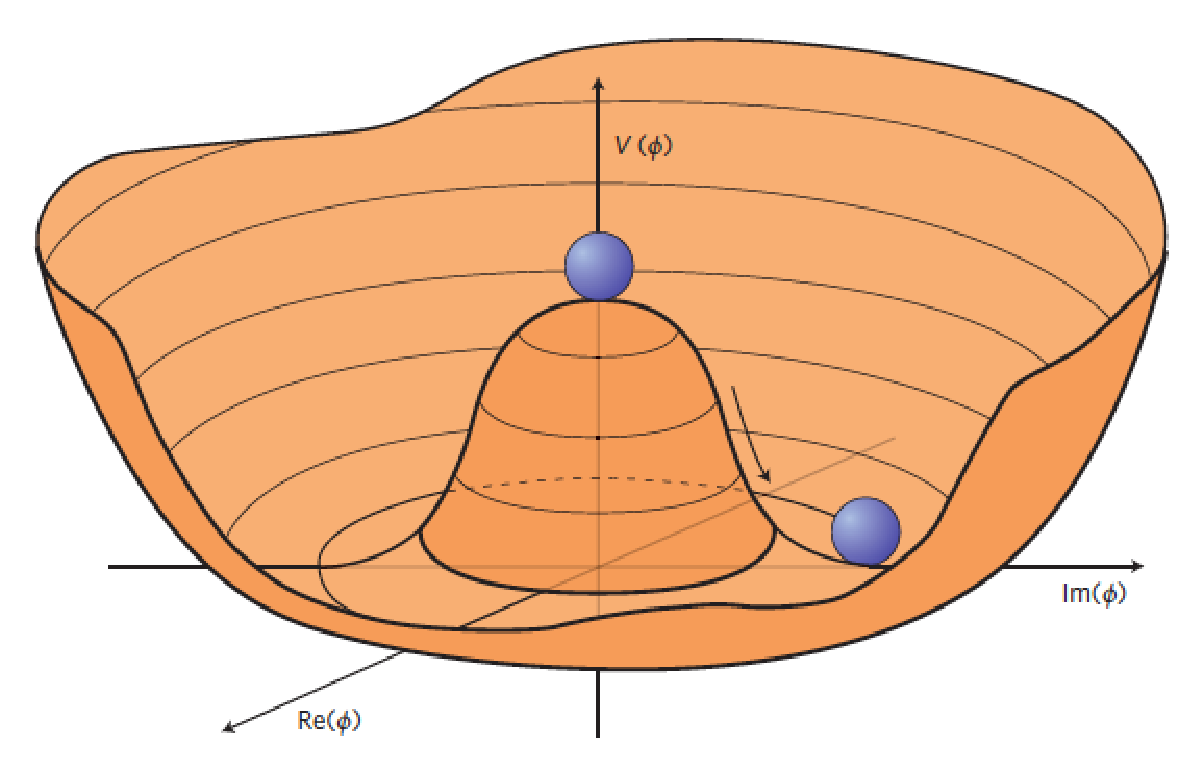
\includegraphics[width=0.75\linewidth]{figures/theory/higgspotential.eps}
\caption{The value of the Higgs potential, $V(\Phi)$ as a function of $\Phi$, for the case that $\mu^2 < 0$ \cite{Ellis:1638469}.}
\label{fig:higgspotential}
\end{figure}

The significant feature of this potential is that its minimum does not occur for a value of $\Phi = 0$. Instead, it is minimized when $|\Phi^\dagger \Phi| = -\mu^2/\lambda$. This means that in its ground state, the Higgs field takes on a non-zero value - referred to as a vacuum expectation value (VEV). So while the Higgs potential is globally symmetric, about the minimum this symmetry is broken. Since the minimum is determined only by $\Phi^\dagger \Phi$, there is some ambiguity in the particular definition of the VEV, but it is generally represented in the unitary gauge as 

\begin{equation}
  \label{eq:VEV}
  \left\langle\Phi\right\rangle = \frac{1}{\sqrt{2}}
  \begin{pmatrix}                                                                                                                               
    0 \\                                                                                                                                   
    v \\                                                                                                                                   
  \end{pmatrix}                                                                                                                       
\end{equation}

The full value of $\Phi$ can be written as 

\begin{equation}                                                                                                                                
  \label{eq:HandV}                                                                                                                                  \left\langle\Phi\right\rangle = \frac{1}{\sqrt{2}}                                                                     
  \begin{pmatrix}                                                                                                                               
    0 \\                                                                                                                   
    v + H\\                                               
  \end{pmatrix}                                                                                                                        
\end{equation}

with $v$ being the value of the VEV, and $H$ being the real value of the scalar field. 

%%%%%%%%%%%%%%%%%%%%%%%%%%%%%%%%%%%%%%%%%%%%%%%%%%%%%%%%%%%%%%%
\subsubsection{Electroweak Symmetry Breaking}
\label{sec:EWKbreaking}

The Electroweak (EWK) interaction is described in the SM by a $SU(2)_L\bigotimes U(1)_Y$ gauge theory. This theory predicts three $SU(2)_L$ gauge boson, $W^1_\mu$, $W^2_\mu$, $W^3_\mu$, and a single $U(1)_Y$ gauge boson, $B_\mu$. The couplings of these bosons to the Higgs field show up in the kinetic terms of the scalar field $\Phi$ in the Lagrangian:

\begin{equation}
  \label{eq:Lphi}
  (D_\mu\Phi)^\dagger(D^\mu\Phi) = |(\partial_\mu - \frac{ig}{2}W^a_\mu\sigma^a - \frac{ig'}{2}B_\mu Y)\phi|^2
\end{equation}

Here $D_\mu$ represents the covariant derivative required to preserve gauge invariance, $g$ and $g'$ represent coupling constant of the gauge bosons, $\sigma^a$ denotes the Pauli matrices of $SU(2)$, and $Y$ represents the hypercharge of $U(1)$. The terms in this interaction which contribute to the masses of the gauge bosons can be written as:

\begin{equation}
  \label{eq:LVEV}
  \frac{1}{2}(0,v)(\frac{g}{2}W^a_\mu\sigma^a - \frac{g'}{2}B_\mu)^2
  \begin{pmatrix}                                                                                                                               
    0 \\                                                                                                                                        
    v \\                                                                                                                                        
  \end{pmatrix}
\end{equation}

Expanding these terms into the mass eigenstates of the electroweak interaction yields four physical gauge bosons, two charged and two neutral, which are linear combinations of the fields $W^1_\mu$, $W^2_\mu$, $W^3_\mu$, and $B_\mu$:

\begin{equation}
\begin{gathered}
  \label{eq:EWKfields}
  W^\pm_\mu = \frac{1}{\sqrt{2}}(W^1_\mu \pm i W^2_\mu) \\
  Z^\mu = \frac{1}{\sqrt(g^2+g'^2)}(-g'B_\mu + gW^3_\mu) \\
  A^\mu = \frac{1}{\sqrt(g^2+g'^2)}(gB_\mu + g'W^3_\mu) \\
\end{gathered}
\end{equation}

And the masses of these fields are given by:

\begin{equation}
\begin{gathered}
  \label{eq:EWKmasses}
  M^2_W = \frac{1}{4}g^2v^2 \\
  M^2_Z = \frac{1}{4}(g^2+g'^2)v^2 \\
  M^2_A = 0 \\
\end{gathered}
\end{equation}

This produces exactly the particles we observe - three massive gauge bosons and a single massless photon. The massless photon represents the portion of the gauge symmetry, a single $U(1)$ of the electromagnetic force, that remains unbroken by the VEV.

Interactions with the Higgs field also lead to the generation of the fermion masses, which in the Lagrangian take the form:

\begin{equation}
  \label{eq:Lfermion}
  y_f (\bar{\psi}_{f,L}\phi \psi_{f,R} + \bar{\psi}_{f,R} \phi^\dagger \psi_{f,L})
\end{equation}

Here $f$ corresponds to each of the fermion flavor, and $y_f$ are matrices containing the Yukawa couplings between the Higgs field and the fermions. After symmetry breaking has occured and $\phi$ has taken on the value of the VEV as written in equation \ref{eq:VEV}, the mass terms of the fermions become $\lambda_\psi v$. Written this way, the fermion masses are proportional to their Yukawa couplings to the VEV, with masses 

\begin{equation}
\label{eq:fMass}
  m_f = y_f\frac{v}{\sqrt{2}}
\end{equation}

Based on the equation \ref{eq:HandV}, an additional mass term arises from the potential $V(\Phi)$. This term can be understood as an excitation of the Higgs field, a scalar boson with mass $m_H = 2\lambda v^2$. This is the Higgs boson, which comes about as a natural prediction of electroweak symmetry breaking. 

The fermions' Yakawa couplings to the VEV take the same form as the fermionss coupling to the Higgs boson. Therefore, the strength of a fermion's interaction with the Higgs is directly proportional to its mass. We now have a model that predicts a Higgs boson with mass $m^2_H = 2\lambda v^2$, which interacts with the fermions with coupling strength $y_f$. Because $\lambda$ and $y_f$ are free parameters of the theory, the mass of the Higgs boson and its interactions with the fermions must be measured experimentally. 

%%%%%%%%%%%%%%%%%%%%%%%%%%%%%%%%%%%%%%%%%%%%%%%%%%%%%%%%%%%%%%%

\subsection{WZ + Heavy Flavor Production}
\label{sec:WZ_theory}

Part \ref{part:wz} is dedicated to a measurement of WZ produced in association with a heavy flavor jet - namely, a charm or b-jet - in the fully leptonic channel. In the instance that both the W and Z bosons decay leptonically, this process produces a final state similar to $t\bar{t}H$, as discussed in section \ref{sec:ttH_theory}, making it an irreducible background for that analysis, and any analysis that includes multiple leptons and b-tagged jets in the final state more broadly.

\begin{figure}[H]
  \centering
  \includegraphics[width=0.35\linewidth]{figures/wz_3l.png}%                                                                 
  \includegraphics[width=0.35\linewidth]{figures/wz_3l_c.png}%                                                               
  \includegraphics[width=0.29\linewidth]{figures/wz_bbar.JPG}
  \caption{Example Feynman diagrams of WZ + heavy flavor production}
  \label{fig:wz_feynman}
\end{figure}

The b-jets produced in this process can be thought of in two different ways: either as originating from the quark ``sea'' of the initial state hadrons, or as the result of a gluon from one the colliding protons splitting into $b\bar{b}$ pairs. However, the heavy flavor contribution to the parton distribution function (PDF) of the proton is uncertain, and simulations of this process disagree depending on which of these two approaches one considers. Regardless of the modelling approach taken, the gluon splitting involved involved in producing the b-quark involves complex QCD calculations that introduce large uncertainties. The same can be said - though to a lesser degree - for charm. This makes WZ + heavy flavor difficult to accurately simulate, and introduces a large uncertainty for any analysis which includes it as a background, motivating a measurement of this process.

This measurement uses 139 $fb^{-1}$ of data collected at a center-of-mass energy of 13 TeV to verify the prediction made by the Sherpa Monte Carlo generator \cite{sherpa} in simulating WZ + heavy flavor production.

%%%%%%%%%%%%%%%%%%%%%%%%%%%%%%%%%%%%%%%%%%%%%%%%%%%%%%%%%%%%%%%

\subsection{$t\bar{t}H$ Production}
\label{sec:ttH_theory}

While the SM has been tested to great precision, particularly at the LHC, it is generally accepted that it is only valid up to a certain energy scale. It is assumed that above a certain energy, at the scale where something like a Grand Unified Theory (GUT) or quantum gravity become relevant, the SM will not be applicable. Further, there are several experimental observations that the SM fails to explain. For example, the SM predicts neutrinos to be massless, despite experimental observation to the contrary, and fails to explain the observation of dark matter and dark energy.

Another example, revelant to the Higgs sector, is known as the hierarchy problem: large quantum corrections to the Higgs mass from loop diagrams, such as those shown in Figure \ref{fig:hierarchyDiagram}, are many orders of magnitude larger than the Higgs mass itself. The observed value of the Higgs mass therefore requires extremely precise cancellation between these corrections and the bare mass of the Higgs, a cancellation which seems unnatural and suggests something missing in our theoretical picture.

\begin{figure}[H]
\centering
   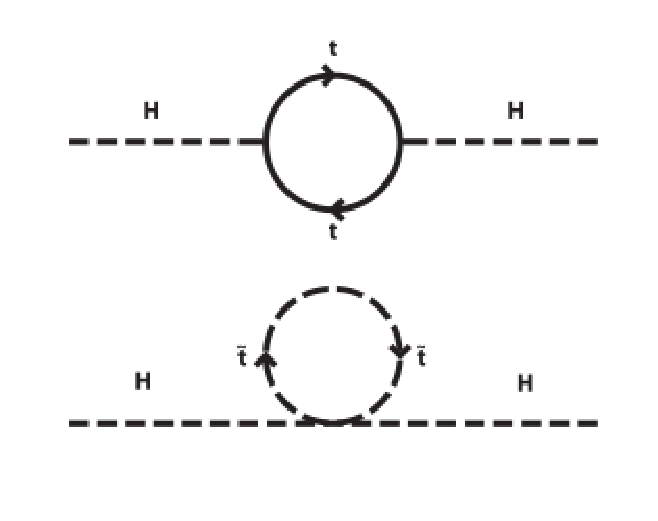
\includegraphics[width=0.5\linewidth]{figures/theory/hierarchyDiagram.eps}
\caption{Above diagram is the leading order correction to the Higgs mass via a top quark loop. Below is a stop squark loop, coming from a supersymmetric extension of the SM which, while not the focus of this paper, is an example of a process that could provide cancellation of the top diagram.}
\label{fig:hierarchyDiagram}
\end{figure}

The strength of a fermion's interaction with the Higgs, given by its Yakawa coupling, is proportionate to its mass. The top quark - as the heaviest known particle - has the strongest interaction, making this interaction particularly interesting to study. While several processes involve interactions between the Higgs and the top, some Higgs production modes include the top interaction only as a part of a loop diagram, such as the gluon-gluon fusion diagram shown in Figure \ref{fig:Hgg}. This process therefore only allows for an indirect probe of the Higgs-top Yakawa coupling, as the flavor of the quark in this diagram is not unique, and can contain other particles.

\begin{figure}[H]
\centering                                                                                                                
   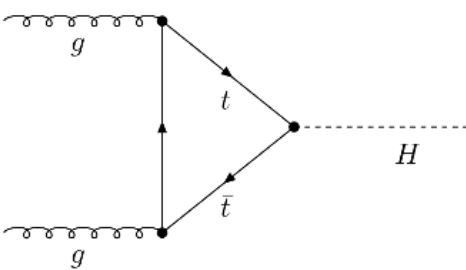
\includegraphics[width=0.5\linewidth]{figures/theory/Hgg.JPG}
\caption{Diagram of a Higgs boson produced via gluon-gluon fusion.}
\label{fig:Hgg}
\end{figure}

Studying the Higgs produced in association with top quark pairs, $t\bar{t}H$, allows this interaction to be measured directly. This process, as shown in Figure \ref{fig:ttH_diagram}, involves a direct coupling between the Higgs and the top, which can be identified by the top quark pair in the final state.

\begin{figure}[H]
\centering
   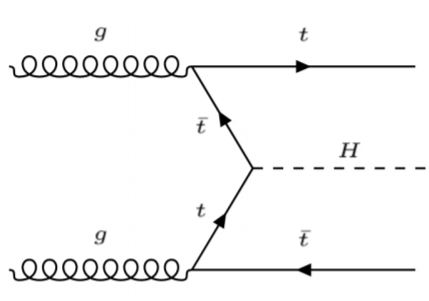
\includegraphics[width=0.6\linewidth]{figures/theory/ttH_diagram.JPG}
\caption{Diagram of a Higgs boson produced in association with a pair of top quarks.}                         
\label{fig:ttH_diagram}                                                                                    
\end{figure}

The Higgs boson, as well as the top quarks, have very short lifetimes - on the order of $10^{-22}$ s and $10^{-25}$ s respectively - meaning they can only be observed via their decay products. Measuring this process is therefore a matter of identifying events with final states consistent with $t\bar{t}H$ production. 

Studies of $t\bar{t}H$ production have been reported by the ATLAS collaboration for $H\rightarrow b\bar{b}$, $H\rightarrow \gamma\gamma$ and multilepton (encompassing $H\rightarrow W^+W^-$, $H\rightarrow ZZ$ and $H\rightarrow \tau^-\tau^+$, with $H\rightarrow ZZ\rightarrow 4l$ as a separate analysis) decay modes. In multilepton final states, at least one of the light leptons, meaning either muons or electrons, originate from the Higgs decay, with other leptons originating from the decay of the top quarks. The channels targeted by this analysis - with 2 same-sign or three leptons in the final state - both involve the Higgs decaying to intermediate W bosons, $H\rightarrow W^+W^-$. The W bosons can decay either to a single lepton and a neutrino, $W\rightarrow l\nu$, providing the source for light leptons, or hadronically into two quarks. The top quarks effectively always decay to a W boson and a b-quark. The W bosons from the top quark decays provide an additional source for final state leptons in $t\bar{t}H$ events.

While the branching ratio of $H\rightarrow W^+W^-$ is smaller than $H \rightarrow b \bar{b}$ (see Table \ref{tab:H_BR}), it produces a clearer signal, as $H \rightarrow b \bar{b}$ suffers from large $t\bar{t}$ backgrounds. On the other hand, $H\rightarrow \gamma\gamma$ produces the most easily identifiable signal, but has a much smaller branching ratio than $H\rightarrow W^+W^-$. Therefore, compared with other final states of $t\bar{t}H$, the $t\bar{t}H-ML$ channel is an attractive candidate for study, as it involves a good balance between statistical power and identifiability. 

\begin{table}[H]
\centering
\begin{tabular}{lc}
\hline\hline
Decay Mode & Branching Ratio (\%) \\
\hline
$H \rightarrow b \bar{b}$ & 58.2 \\
$H\rightarrow WW^*$ & 21.4 \\
$H\rightarrow gg$ & 8.19 \\
$H\rightarrow \tau\tau$ & 6.27 \\
$H\rightarrow c\bar{c}$ & 2.89 \\
$H\rightarrow ZZ^*$ & 2.62 \\
$H\rightarrow \gamma\gamma$ & 0.227 \\
\hline
\end{tabular}
\label{tab:H_BR}
\caption{Summary of the predominant SM Higgs ($m_H = 125$ GeV) branching ratios. Particles with a star imply off-shell decays.}
\end{table} 

Searches for $t\bar{t}H$ production typically target a measurement of the signal strength parameter, $\mu_{t\bar{t}H}$, which measures the ratio of the observed rate and the expected rate according to the SM prediction.

\begin{equation}
        \mu_{t\bar{t}H} = \frac{\sigma^{obs.}_{t\bar{t}H}}{\sigma^{SM}_{t\bar{t}H}}
\end{equation}

$t\bar{t}H$ production was observed by ATLAS using up to 79.8 $fb^{-1}$ of data collected at $\sqrt{s}$ = 13 TeV, based on a combination of five Higgs decay modes: $b\bar{b}$, $WW^*$, $\tau^{-}\tau^{+}$, $\gamma\gamma$, and $ZZ^*$ \cite{Higgs_combo}. A significance of $5.8\sigma$ was observed, compared to a $4.9\sigma$ expected significance. Since then, two analyses have published updated results ($H\rightarrow \gamma\gamma$ and $H\rightarrow ZZ^*\rightarrow 4l$) with the full Run 2 dataset, representing 139 $fb^{-1}$. Studies are still ongoing in the remaining channels.

The CMS collaboration has performed similar searched for $t\bar{t}H$, acheiving an observed (expected) significance of 5.2$\sigma$ (4.2$\sigma$) across each of the Higgs decay modes using data collected from 2011-2017 with center of mass energies of 7, 8, and 13 TeV \cite{PhysRevLett.120.231801}. 

%%%%%%%%%%%%%%%%%%%%%%%%%%%%%%%%%%%%%%%%%%%%%%%%%%%%%%%%%%%%%%%

\subsection{Differential Measurements of $t\bar{t}H$}
\label{sec:bsm}

While $t\bar{t}H$ has been observed by both the ATLAS \cite{ttH_paper} and CMS \cite{Sirunyan_2018} collaborations, these analyses have focused on measuring the overall rate of $t\bar{t}H$ production. There are several theories of physics Beyond the Standard Model (BSM), however, that could affect the kinematics of $t\bar{t}H$ production without significantly altering its overall rate \cite{Dumont_2013}.

An Effective Field Theory approach can be used to model the low energy effects of new, high energy physics, by paramaterizing BSM effects as higher dimensional operators. These additional operators can then be added to the SM Lagrangian to write an effective Lagrangian that accounts for the effects of these higher energy physics. The lowest order of these that could contribute to Higgs-top coupings are dimension-six, as represented in Equation \ref{eq:dim6}.

\begin{equation}
\label{eq:dim6}
\mathcal{L}_{eff} = \mathcal{L}_{SM} + \frac{f}{\Lambda}\mathcal{O}^6
\end{equation}

Here $\Lambda$ represents the energy scale of the new physics, $f$ is a Wilson coefficient which represents the strength of the effective coupling, and $\mathcal{O}$ is the operator. An experimental observation of any non-zero value of $f$ would be a sign of BSM physics.

The addition of these operators can be shown to modify the transverse momentum ($p_T$) spectrum of the Higgs Boson in Higg-top interactions, without significantly affecting the overall rate of $t\bar{t}H$ production \cite{Banerjee_2014}. The possible impact of these higher order effects on the Higgs $p_T$ spectrum are shown in Figure \ref{fig:eft_pt}. Here the additional operators include an effective quartic coupling between the gluon, Higgs, and a pair of top quarks, the strength of which is represented by $C_{ght}$, and a loop-induced interaction between the gluon and Higgs, $C_{GH}$. In this example the parameters are chosen such that the overall rate of $t\bar{t}H$ production remains the same as the Standard Model prediction.

\begin{figure}[H]
\centering
   \includegraphics[width=0.5\linewidth]{figures/theory/higgs_pt.PNG}
\caption{The momentum spectrum of the Higgs boson produced via top-quarks with (red) and without (blue) the presence of a particular choice of dimension-six operator.  \cite{Banerjee_2014}.}
\label{fig:eft_pt}
\end{figure}

Here the additional operators include an effective quartic coupling between the gluon, Higgs, and a pair of top quarks, shown in Equation \ref{eq:gtth}, the strength of which is represented by $C_{ght}$. $C_{GH}$ is the strength of a loop-induced interaction between the gluon and Higgs \ref{eq:gh}. In this example the values of these couplings are chosen such that the overall rate of $t\bar{t}H$ production remains the same as the Standard Model prediction.

\begin{equation}
\label{eq:gtth}
(\tilde{q}\sigma^{\mu\nu}T^At)\tilde{\phi}G^A_{\mu\nu}
\end{equation}


\begin{equation}
\label{eq:gh}
(\phi^\dagger\phi)G^A_{\mu\nu}G^{A\mu\nu}
\end{equation}


This provides a clear, physics observable that could be used to search for evidence of BSM physics using data collected at the LHC. Reconstructing the momentum spectrum of the Higgs in $t\bar{t}H$ events therefore provides a means to search for new physics in the Higgs sector.

Reconstructing the Higgs is a particular challenge in the multilepton channels of $t\bar{t}H$, due to an ambiguity arising from multiple sources of missing energy. In the $H\rightarrow \gamma\gamma$ channel, the kinematics of the Higgs can be fully reconstructed from the two photons. The same is true of $H\rightarrow b\bar{b}$, though with the additional challenge of identifying which two of the four b-quarks in the final state originated from the Higgs. By contrast, the two channels ($2lSS$ and $3l$) targeted by this analysis include at least one neutrino originating from the Higgs decay. 

\begin{figure}[H]
    \centering
    \subfigure[]{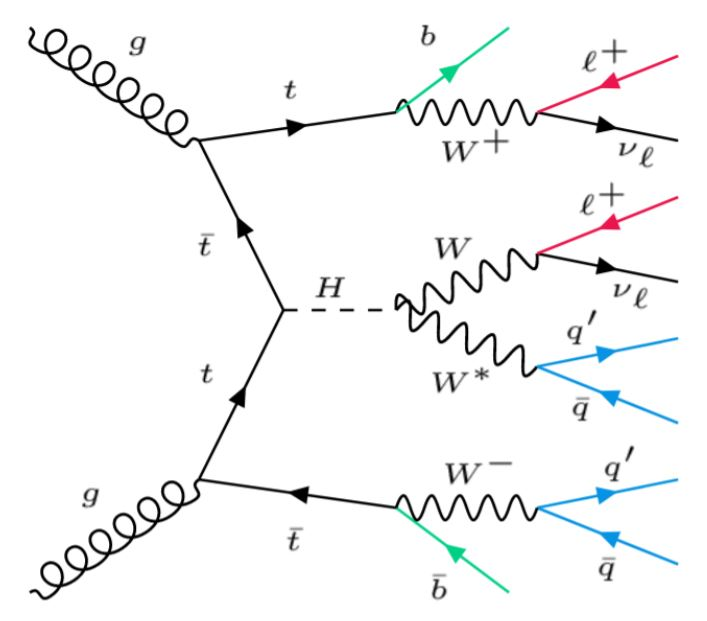
\includegraphics[width=.43\linewidth]{theory/ttH-2lSS.JPG}}%                             
    \subfigure[]{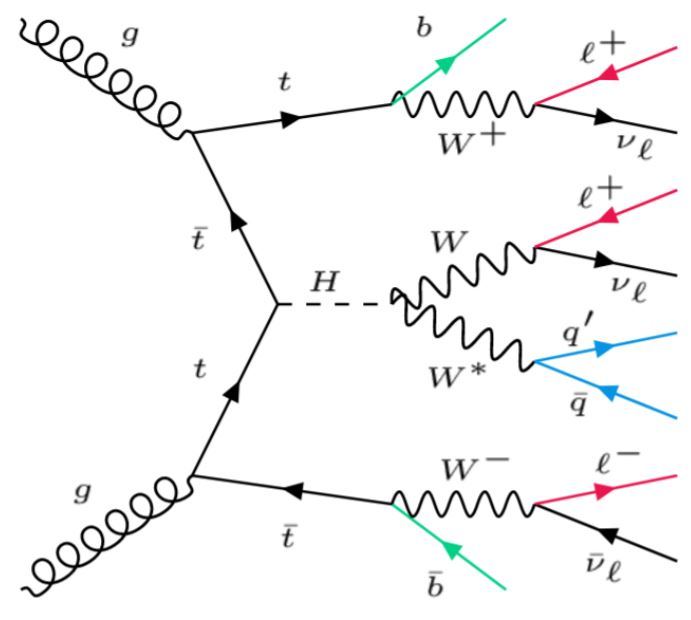
\includegraphics[width=.43\linewidth]{theory/ttH-3l.JPG}}%                                
    \caption{Feynman diagrams of $t\bar{t}H$ production with (a) two same-sign leptons and (b) three leptons in the final state.}
    \label{fig:ttH-2lSS-3l}
\end{figure}

Neutrinos are not detected by ATLAS; instead, their presence is inferred from missing transverse energy in the detector, $E^T_{miss}$. The two channels targeted here include not just a neutrino from the Higgs decay, but at least one additional neutrino from the decay of the top-quarks. This makes disentangling the contribution of the Higgs decay to $E^T_{miss}$, and thereby fully reconstructing the Higgs, impossible. This challenge motivates the use of more sophisticated machine learning techniques when attempting to perform differential measurements of the Higgs $p_T$ spectrum in the multi-lepton channels of $t\bar{t}H$. 

Chapter \ref{part:analysis} provides exploratory studies on the feasibility of differential measurements of $t\bar{t}H-ML$, specifically targeting events with two same-sign leptons ($2lSS$) or three leptons ($3l$) in the final state. This includes $H \rightarrow W^+W^-$ events, where at least one of the W bosons decays leptonically. The techniques used to reconstruct the Higgs transverse momentum spectrum are explained, and preliminary results are shown for data collected by ATLAS from 2015-2017, with projected results shown for the full 2015-2018 dataset.

%%%%%%%%%%%%%%%%%%%%%%%%%%%%%%%%%%%%%%%%%%%%%%%%%%%%%%%%%%%%%%% 


\index{The Standard Model and the Higgs Boson@\emph{The Standard Model and the Higgs Boson}}% 
%------------------------------------------------------------------------------

%\section{Effective Field Theory in $t\bar{t}H$ Production}
%\label{sec:eft}
%Higher dimension operators are a common way to paramaterize the effects of physics at very high energies into

\subsection{Extensions to the Higgs Sector}
\label{sec:higgsExt}

%%%%%%%%%%%%%%%%%%%%%%%%%%%%%%%%%%%%%%%%%%%%%%%%%%%%%%%%%%%%%

\subsection{Six Dimensional Operators}
\label{sec:dim6}

While the SM has been tested to great precision, particularly at the LHC, it is generally accepted that it is only valid up to a certain energy scale. It is assumed that above a certain energy, at the scale where something like a Grand Unified Theory (GUT) or quantum gravity become relevant, the SM will not be applicable. 


%------------------------------------------------------------------------------

%-------------------------------------------------------------------------------
%-------------------------------------------------------------------------------

\chapter{The LHC and the ATLAS Detector}
\label{part:lhcAtlas}

%-------------------------------------------------------------------------------

\section{The LHC}
\label{sec:lhc}
\index{The LHC@\emph{The LHC}}
The Large Hadron Collider (LHC) is a particle accelerator consisting of a 27 km ring, designed to collide protons at high energy. Located outside of Geneva, Switzerland and buried about 100 m undergound, it consists of a ring of superconducting magnets which are used to accelerate opposing beams of protons - or lead ions - which collide at the center of one of the various detectors located around the LHC ring which record the result of these collisions. These detectors include two general purpose detectors, ATLAS and CMS, which are designed to make precision measurements of a broad range of physics phenomenon, and two more specialized experiments, LHCb and ALICE, which are optimized to study b-quarks and heavy-ion physics, respectively.

The LHC first began running in 2009 at a proton-proton center of mass energy of $\sqrt{s} = 8$ TeV. It operated at this energy from 2009 to 2012, known as Run 1, and data collected during this period was used in discovering the Higgs Boson. The LHC began running again in 2015, and collected data at an increased energy of $\sqrt{s} = 13$ TeV until 2018, a period referred to as Run 2. 

The LHC consists of a chain of accelerators, which accelerate the protons to higher and higher energies until they are injected into the main ring. This process is summarized in figure \ref{fig:AccChain}. Protons extracted from a tank of ionized hydrogen are fed into a linear accelerator, LINAC2, where they reach an energy of 50 MeV. From there, they enter a series of three separate circular accelerators, before being injected into the main accelerator ring at an energy of 450 GeV. Within the main ring protons are seperated into two seperate beams moving in opposite directions, and their energy is increased to their full collision energy. Radiofrequency cavities are used to accelerate these particles are sort them into bunches. From 2015-2018, these bunches consisted of around 100 billion protons each with an energy of 6.5 TeV per proton, which collided at a rate of 40 MHz, or every 25 ns. 

\begin{figure}[H]
\centering
   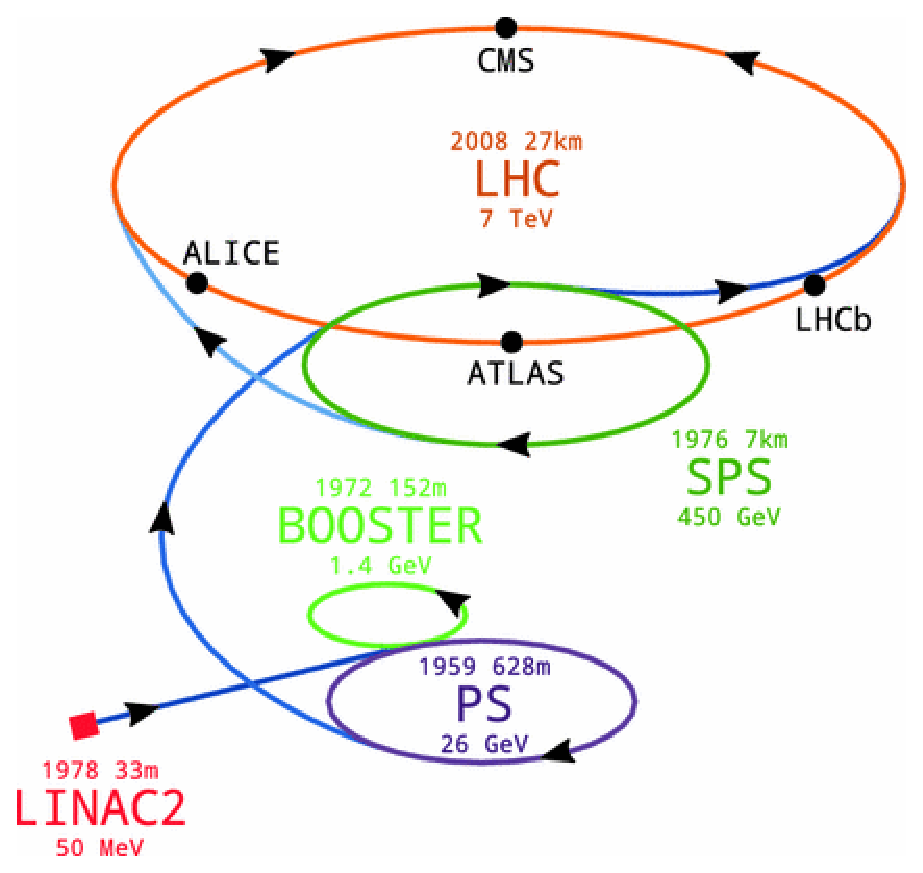
\includegraphics[width=0.75\linewidth]{figures/lhc/AccChain.eps}
\caption{A summary of the accelerator chain used to feed protons into the LHC \cite{}.}
\label{fig:AccChain}
\end{figure}

Because these proton bunches consist of a large number of particles, each bunch crossing consists of not just one, but several direct proton-proton collisions. The number of interactions that occur per bunch crossing, $\mu$, is known as pileup. During Run 2, the average pileup for bunch crossings was around $\left\langle\mu\right\rangle$ = 35, with values typically ranging between 10 and 70.

The amount of data collected by the LHC is measured in terms of luminosity, which is the ratio of the number of events detected per unit time, $\frac{dN}{dt}$, and the interaction cross-section, $\sigma$. 

\begin{equation}                                                                                                                                
        \label{eq:lumiDef}                                                                                                                      
        \mathcal{L} = \frac{1}{\sigma}\frac{dN}{dt}
\end{equation}

The design luminosity of the LHC is $10^{34}\ cm^{-2}s^{-1}$, however the LHC has acheived a luminosity of over $2\times 10^{34}\ cm^{-2}s^{-1}$. The total luminosity is then this instantaneous luminosity integrated over time.

\begin{equation}
        \label{eq:intLumi}      
        \mathcal{L}_{int} = \int\mathcal{L}dt
\end{equation}

The integrated luminosity collected by the ATLAS detector as of the end of 2018 is around 140 $fb^{-1}$, exceeding the expected integrated luminosity of 100 $fb^{-1}$.
                                            
                                         


%------------------------------------------------------------------------------

\section{The ATLAS Detector}
\label{sec:atlas}
ATLAS (a not terribly natural acronym for ``A Toroidal LHC Apparatus'') is a general purpose detector designed to maximize the detection efficiency of all physics objects, including leptons, jets, and photons. This means it is capable of measuring all SM particles, with the exception of neutrinos, the presence of which can be inferred based on missing transverse momentum. The detector measures 44 m long, and 25 m tall. 

The ATLAS detector consists of multiple layers, each of which serves a different purpose in reconstructing collisions. At the very center of the detector is the interaction point where the proton beams of the LHC collide. 

\begin{figure}[H]
\centering
   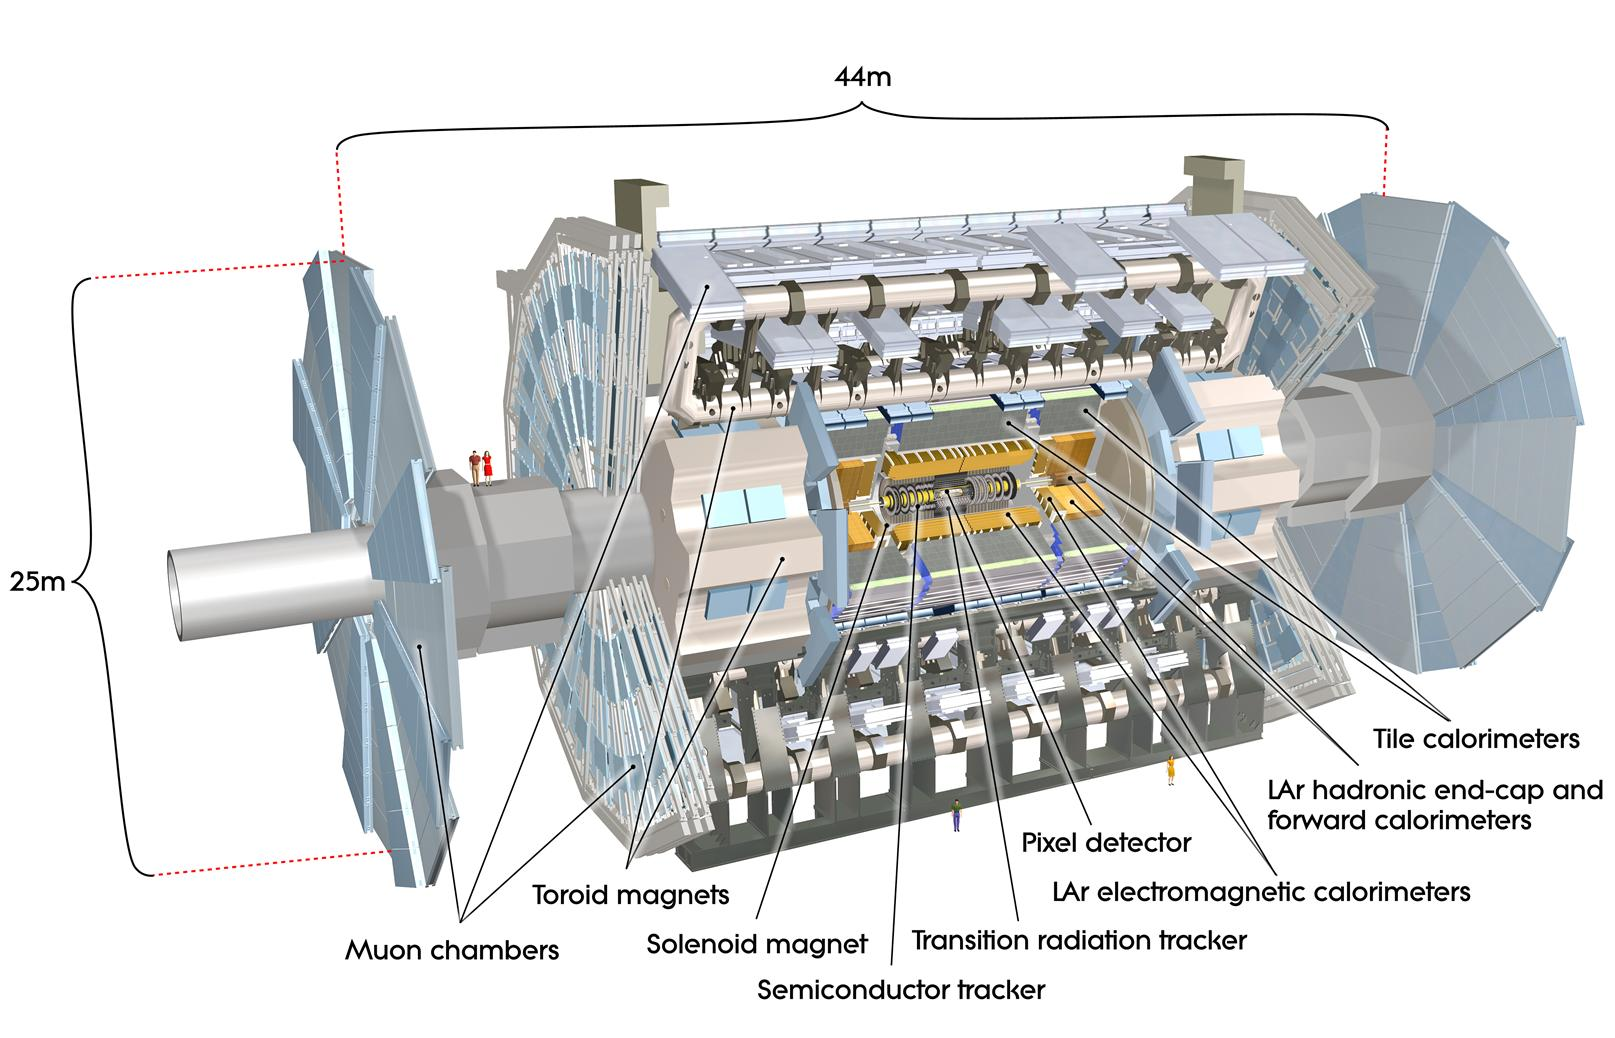
\includegraphics[width=0.75\linewidth]{figures/lhc/ATLASdiagram.eps}
\caption{Cutaway view of the ATLAS detector, with labels of its major components \cite{ATLAS_figure}.}
\label{fig:ATLAS}
\end{figure}

\subsection{Inner Detector}
\label{sec:innerDetector}

\begin{figure}[H]
\centering
   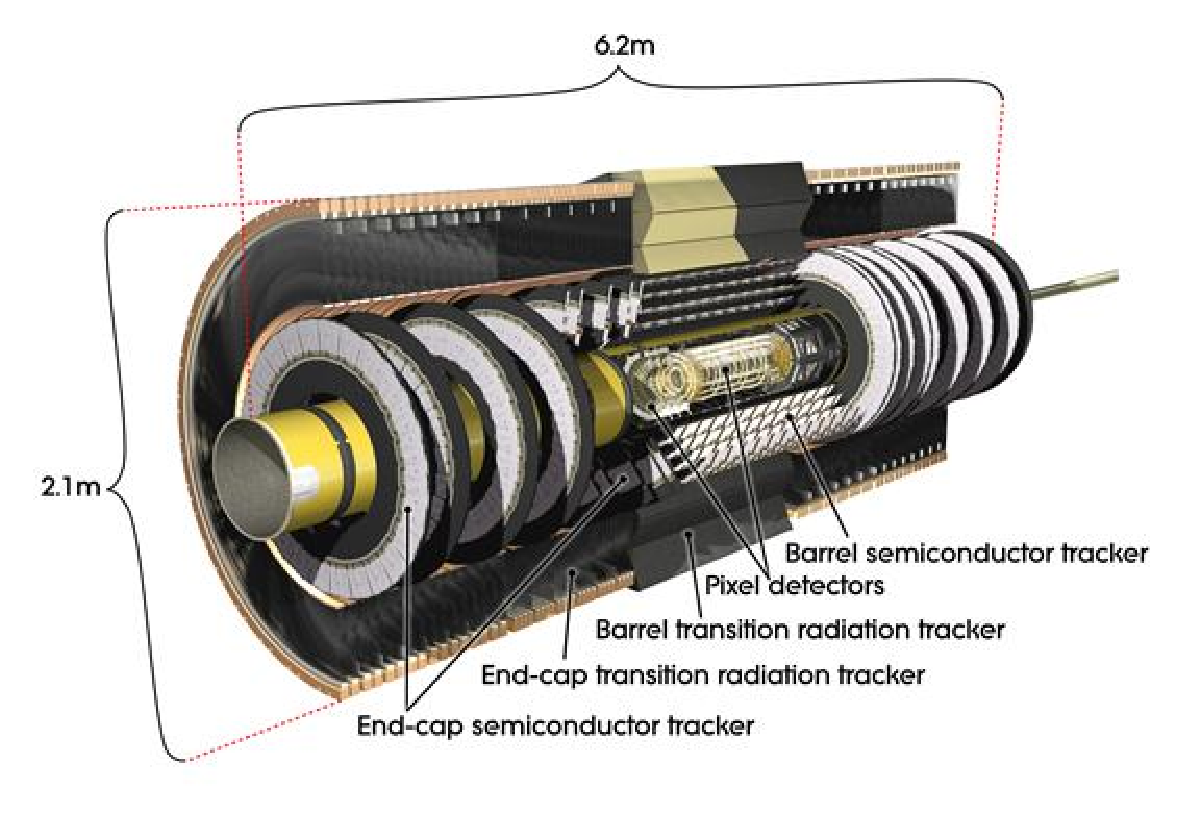
\includegraphics[width=0.75\linewidth]{figures/lhc/InnerDetector.eps}
\caption{Cutaway view of the Inner Detector \cite{caloFig}.}
\label{fig:innerDect}
\end{figure}

Just surrounding the interaction point is the Inner Detector, designed to track the path of charged particles moving through the detector. An inner solenoid surrounding the Innder Detector is used to produces a magnetic field of 2 T. This large magnetic field causes the path of charged particles moving through the Inner Detector to bend. Because this magnetic field is uniform and well known, it can be used in conjunction with the curvature of a particles path to measure its charge and momentum.

The Inner Detector consists of three components - the Pixel Detector, the Semi-Conductor Tracker (SCT), and the Transition Radiation Tracker (TRT). The Pixel Detector is the innermost of these, beginning just 33.25 mm away from the beam line. It consists of three silicon layers along the barrel, as well as three endcap layers, covering a range of $|\eta|$ < 2.5. 

The Semiconductor Tracker (SCT) is similar to the Pixel detector, but uses long strips rather than small pixel to cover a larger spatial area.

\subsection{Calorimeters}
\label{sec:calo}

\begin{figure}[H]
\centering
   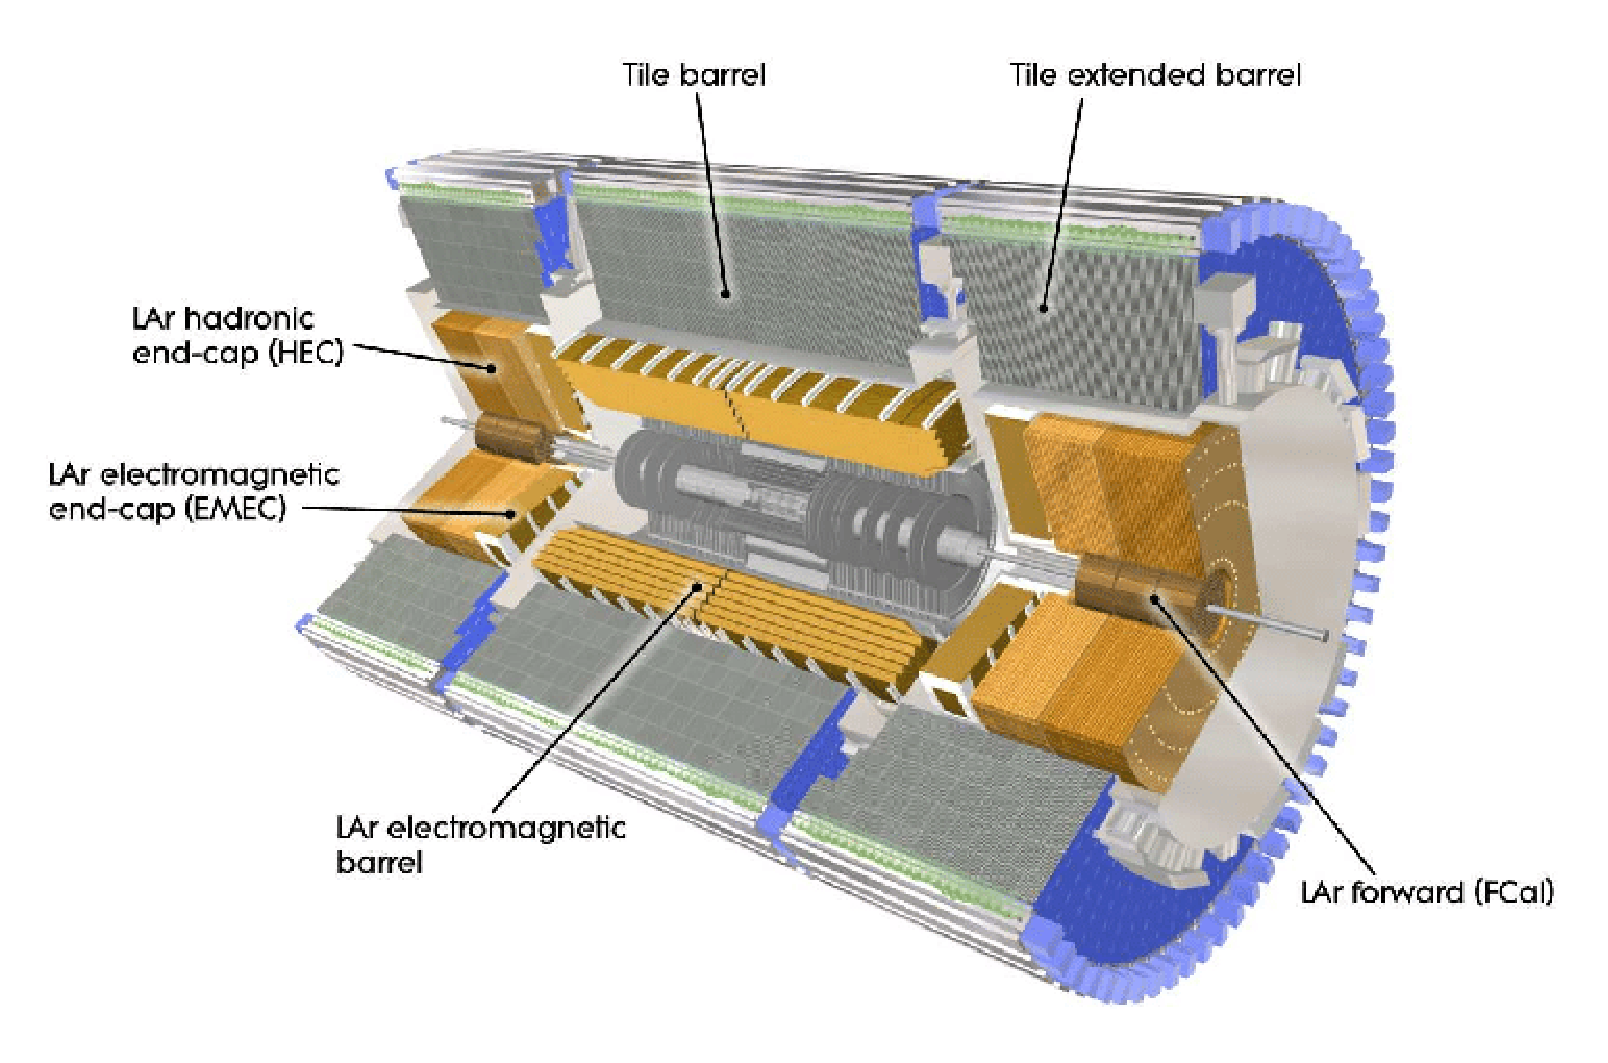
\includegraphics[width=0.9\linewidth]{figures/lhc/calorimeter.eps}
\caption{Cutaway view of the calorimeter system of the ATLAS detector \cite{caloFig}.}
\label{fig:calo}
\end{figure}

Situated outside the Innder Detector are two concentric calorimeters. The inner calorimeter uses liquid argon (LAr) to measure energy of particles the interact electromagnetically, which includes photons and any charged particle. The LAr calorimeter is made of heavy metals, primarily lead and copper, which causes electromagnetically interacting particles to shower, depositing their energy in the detector. The showering of the high energy particles that pass through calorimeter cause the liquid argon to ionize, and the ionized electrons are detected by electronic readouts. The LAr calorimeter consists of around 180,000 readout channels.  

The outer calorimeter measures the energy from particles that pass through the EM calorimeter, and measures the energy of particles that interact via the strong force. This is primarily hadrons. It is composed of steel plates to cause hadronic showering and scintillating tiles as the active material. The signals from the hadronic calorimeter are read out by photomultiplier tubes (PMTs).

\subsection{Muon Spectrometer}
\label{sec:muonSpec}

Because muons are heavier than electrons and photons, and do not interact via the strong force, they generally pass through the detector without being stopped by the calorimeters. The outermost components of the detector are designed specifically to measure the energy and momentum of muons produced in the LHC. The muon spectrometer consists of tracking and triggering system. It extends from the outside of the calormeter system, about a 4.25 m radius from the beam line, to a radius of 11 m. This large detector system is necessary to accurately measure the momentum of muons, which is essential not only for measurements involving the muons themselves, but also to accurately estimate the missing energy in each event.

Two large toroidal magnets within the muon system generate a large magnetic field which covers an area 26 m long with a radius of 10 m. Because the area covered by this magnet system is so large, a uniform magnetic field like the one produced in the Inner Detector is impractical. Instead, the magnetic field that exists in the muon spectrometer ranges between 2 T and 8 T, and is much less uniform. The path of the muons passing through the spectrometer is bent by this field, allowing their charge to be determined. 

1200 tracking chambers are placed in the muon system in order to precisely measure the tracks of muons with high spatial resolution.

%\subsection{Forward Detector}
%\label{sec:forwardDet}

\subsection{Trigger System}
\label{sec:trigger}

Because of the high collision rate and large amount of data collected by the various subdetectors, ATLAS produces far more data than can actually be stored. Each event produces around 25 Mb of raw data, which multiplied by the bunch crossing rate of 40 MHz, comes out to around a petabyte of data every second. The information from every event cannot practically be stored, therefore a sophisticated trigger system is employed in real time to determine whether events are sufficiently interesting to be worth storing.

The trigger system in ATLAS involves multiple levels, each of which select out which events move on to the next level of scrutiny. The level-1 trigger uses hardware information from the calorimeters and muon spectrometer to select events that contain candidates for particles commonly used in analysis, such as energetic leptons and jets. The level-1 trigger reduces the rate of events from 40 MHz to around 100 kHz. 

Events that pass the level-1 trigger move to the High-Level Trigger (HLT). The HLT takes place outside of the detector in software, and looks for properties such as a large amount of missing transverse energy, well defined leptons, and multiple high energy jets. Events that pass the HLT are stored and used for analysis. Because the specifics of the HLT are determined by software rather than hardware, the thresholds can be changed throughout the run of the detector in response to run conditions such as changes to pilup and luminosity. After the HLT is applied, the event rate is reduced to around 1000 per second, which are recorded for analysis.


%------------------------------------------------------------------------------
%-------------------------------------------------------------------------------                                             
\chapter{Object Definition and Data Samples}
\label{part:objMC}

%------------------------------------------------------------------------------- 
\section{Object Identification and Reconstruction}
\label{sec:objID}

This section decribes the reconstruction of the physics objects relevant to these analyses, as well as the selection applied to these objects. This selection and object definition is shared between both analyses presented. This includes the reconstruction and selection of light leptons and jets, the determination of missing energy in each event ($E_T^{miss}$), the algorithms used to identify jets originating from $b$-hadrons ($b$-tagging), and the procedure used to resolve ambiguities between physics objects, known as overlap removal.

\subsection{Electrons}
\label{obj:ele}

Electron candidates are reconstructed from energy clusters in the electromagnetic (EM) calorimeter that are associated with charged particle tracks reconstructed in the inner detector~\cite{ATLAS-CONF-2016-024}. Electron candidates are required to fall within the pseudorapidity region $|\eta| < 2.5$, excluding the transition region between the barrel and end-cap of the EM calorimeter, $1.37 < |\eta_\textrm{cluster}| < 1.52$, where there is a large fraction of inactive material. 

Electron reconstruction begins by identifying energy clusters in the EM calorimeter. The EM calorimeter is divided into a grid of ``towers'', each covering a solid angle of $\Delta\eta\times\Delta\phi = 0.025\times 0.025$, corresponding to the resolution of the calorimeter. A sliding windows algorithm, with clusters of $3\times 5$ towers, is used to traverse the phase space of the calorimeter. Candidates are formed from these clusters which represent a local maximum and transverse energy more than 2.5 GeV. If two cluster which overlap within an area of $5\times 9$, the higher energy cluster is kept.

Once cluster candidates are identified, they are matched to tracks from the inner detector. This association is performed by comparing the $\eta$ and $\phi$ values of the tracks to the energy clusters, which must fall within $|\Delta\eta| < 0.05$ and $-0.10 < \Delta\phi < 0.05$. The assymetric $\phi$ condition is chosen to account for the energy loss of charged particles whose tracks bend through the magnetic field of the inner detector. If multiple tracks match a single cluster, a primary track is chosen based on the number of hits in the pixel and silicon layers of the tracker, and whether the track originates from a secondary vertex.

Measurements involving electrons must correct for the reconstruction efficiency of electrons, which is calculated directly using a data driven tag-and-probe method \cite{tagAndProbe}. This involed using a precisely known physics process, $Z\rightarrow e^+e^-$, to calculate the electron efficiency of the detector. An extremely high electron reconstruction efficiency is found, as shown in Figure \ref{fig:eEffEt}.

\begin{figure}[H]
\centering
   \includegraphics[width=0.65\linewidth]{figures/theory/eEffEt.JPG}
\caption{Electron reconstruction efficiency as a function of electron transverse energy for $Z\rightarrow e^+e^-$ events \cite{tagAndProbe}.}
\label{fig:eEffEt}
\end{figure}

Electrons which are reconstructed pass through to an electron identification step, described in \cite{tagAndProbe}. Electron identification attempts to select prompt electrons using properties of the ID tracks and EM clusters of electron candidates.  A likelihood approach is used to form working points (WPs) of decreasing electron efficiency, but increasing prompt electron purity: Loose, Medium, and Tight. More restrictive WPs can be used to reduce the contributions of fake and non-prompt electrons. As with reconstruction, the tag-and-probe method is used to calculate the electron efficiency of each of these WPs. 

\begin{figure}[H]
\centering
   \includegraphics[width=0.65\linewidth]{figures/theory/eEffEt.JPG}
\caption{Electron identification efficiency for Loose, Medium, and Tight WPs as a function of electron transverse energy for $Z\rightarrow e^+e^-$ events \cite{tagAndProbe}.}
\label{fig:eEffEt}
\end{figure}

Electrons are required to pass the tight identification working point to minimize non-prompt backgrounds. To further reduce the non-prompt contribution, the track of each electron is required to originate from the primary vertex; requirements are also imposed on the transverse impact parameter significance ($|d_0|/\sigma_{d_0}<5$) and the longitudinal impact parameter ($|\Delta z_0 \sin \theta_\ell|<0.5$ mm).

Electron and muons are required to pass a non-prompt BDT selection developed by the main $t\bar{t}H$/$t\bar{t}W$ analysis, described in detail in \cite{ttH_paper}. Optimized working points and scale factors for this BDT are taken from that analysis. This BDT and the WPs used are summarized in Appendix \ref{sec:lepMVA},

\subsection{Muons}
\label{obj:muon}
                   
The reconstruction algorithm for Combined Muons is used, where muon candidates are reconstructed by combining inner detector tracks with track segments or full tracks in the muon spectrometer (MS) \cite{PERF-2014-05}. Only muons which fall within a range of $|\eta| < 2.5$ are considered. Similar to electrons, an outside-in approach is used, where muon tracks are first identified in the MS, which are then matched to tracks from the inner detector. Muons which fall in the region $|\eta| < 0.1$, where muon spectrometer coverage is reduced, are matched to energy clusters in the calorimeter as well.

Muon identification is used to suppress non-prompt muons, and ensure robust momentum measurements. The Medium identification WP is used for muons in this case. Medium ID cuts require at least one Pixel hit, five SCT hits, fewer than three Pixel or SCT holes, and that at least 10\% of the TRT hits originally assigned to the track are included. A hole is defined as an active sensor traversed by the track but containing no hits. A missing hit is considered a hole only when it falls between hits successfully assigned to a given track. Again, a tag-and-probe method is used in order to calculate the reconstruction efficiency of muons.

\begin{figure}[H]
\centering
   \includegraphics[width=0.65\linewidth]{figures/theory/muonID.JPG}
\caption{Muon reconstruction efficiency for Medium ID muons as a function of transverse energy for $Z\rightarrow \mu\mu$ and $J/\psi\rightarrow\mu\mu$ events \cite{PERF-2014-05}.}
\label{fig:eEffEt}
\end{figure}

In addition to requiring muons pass the non-prompt BDT, requirements are imposed on the transverse impact parameter significance ($|d_0|/\sigma_{d_0}<3$) and the longitudinal impact parameter ($|\Delta z_0 \sin \theta_\ell|<0.5$ mm).
 
\subsection{Non-prompt lepton MVA}
\label{sec:lepMVA}
\input{wz_sections/lepMVA}

\subsection{Jets}
\label{obj:jets}

The nature of the strong force prevents quarks produced in collisions from being measured directly; instead, free quarks produce many quark-antiquark pairs, or hadrons. This process is called hadronization. The tight cone of particles - consisting primarily of charged pions, charged kaons, photons from $\pi^0$ decays, and neutral hadrons - produced from the hadronization of a quark or gluon is referred to as a jet. Jets, rather than quarks, are what is observed by the detector.

Jet reconstruction algorithms are designed to group these particles together in order to measure information about the initial quark. Traditional jet reconstruction algorithms involve clustering energy deposits from the calorimeter systems, (Calorimeter-jets) \cite{PERF-2015-05}. Soft proton-proton collisions in an event aside from the primary collision, known as pileup, can create a background of particles that the calorimeter alone cannot differentiate, introducing a significant limitation to Calorimeter-jets. Instead, a jet clustering algorithm called ``Particle-Flow'', or PFlow, is used for this work \cite{PERF-2015-09}. PFlow jets use tracking information in addition to calorimeter information in order to more effectively filter out contributions from pileup.

For these analyses, jets are reconstructed from calibrated topological clusters built from energy deposits in the calorimeters \cite{ATL-PHYS-PUB-2015-015}, as well as information from the inner tracking detector, using the anti-$k_t$ algorithm with a radius parameter $R=0.4$. Jets with energy contributions likely arising from noise or detector effects are removed from consideration \cite{ATLAS-CONF-2015-029}, and only jets satisfying $p_T > 25$~GeV and $|\eta| < 2.5$ are used in this analysis.

The predominant uncertainties in jet measurement fall into two categories: jet energy scale (JES) and jet energy resolution (JER). JES is a scaling constant between the strength of the output voltage of the detector and the energy of the jet in GeV \cite{atlascollaboration2020jet}. JES is calibrated using well measured objects such as leptons and $Z$ bosons in order to match expected energy output to the detector response. The JES uncertainty as a function of jet $p_T$ is shown in figure \ref{fig:jesUnc}.

\begin{figure}[H]
\centering
   \includegraphics[width=0.65\linewidth]{figures/theory/jesUnc.JPG}
\caption{Jet energy scale uncertainty as a function of jet $p_T$ \cite{atlascollaboration2020jet}}
\label{fig:jesUnc}
\end{figure}

Jet energy resolution is the uncertainty on individual jet energy measurements from fluctuations in jet composition, detector resolution, and uncertainty in jet reconstruction algorithms. The JER uncertainty as a function of jet $p_T$ is shown in figure \ref{fig:jerUnc}.

\begin{figure}[H]
\centering
   \includegraphics[width=0.65\linewidth]{figures/theory/jerUnc.JPG}
\caption{Jet energy resolution uncertainty as a function of jet $p_T$ \cite{atlascollaboration2020jet}}
\label{fig:jerUnc}
\end{figure}

\subsection{$b$-tagging}
\label{obj:bjets}

$b$-tagging is the process of distinguishing jets that originate from $b$-quarks from jets that originate from lighter flavor quarks. $b$-hadrons formed from $b$-quarks have a relatively long lifetime compared to other hadrons, which, in addition to Lorentz boosting, means they travel several millimeters in the detector before decaying to other hadrons. Therefore $b$-jets will originate from an additional vertex several millimeters from the primary interaction point. Identifying this secondary vertex is a key component of $b$-tagging.

The $b$-tagging algorithm consists of a two-step approach, with the first designed to reconstruct the characteristic properties of $b$-jets, using track information to reconstruct displaced veritces \cite{Heer:2017kbn} and other key $b$-tagging information. The output of this first step is combined with additional jet information as inputs to a high level tagger.

In this case, the DL1r $b$-tagging algorithm is used. The DL1r algorithm \cite{btag_cal} uses jet kinematics, particularly jet vertex information, as input for a neural network which assigns each jet a score designed to reflect how likely that jet is to have originated from a b-quark. 

\begin{figure}[H] 
    \centering
    \includegraphics[width=0.54\linewidth]{DL1_output.pdf} 
    \caption{Output distribution of the DL1r algorithm for pure samples of $b$-jets, charm jets, and light jets, with each normalized to unity \cite{btag_cal}}
    \label{fig:DL1r}
\end{figure}

From the output of the BDT, working points (WPs) are developed based on the efficiency of truth b-jets at particular values of the DL1r algorithm. The working points used in this analysis are summarized in Table \ref{tab:btag_WPs}. 

\begin{table}[H] 
\begin{center}
\begin{tabular}{|c|c|c|}
     \hline
    WP & \multicolumn{2}{c|}{Rejection}\\
    \hline
    $b$-jet eff. & $c$-jet & light jet\\
    \hline
     85\% & 2.6 & 29 \\
     77\% & 4.9 & 130 \\
     70\% & 9.4 & 390 \\
     60\% & 27 & 1300 \\
     \hline
     \end{tabular}
    \caption{$c$-jet and light-flavor jet rejections corresponding to each $b$-tagging Working Point by b-jet efficiency, evaluated on $t\bar{t}$ events.}
     \label{tab:btag_WPs}
     \end{center}
\end{table}

As shown in table \ref{tab:btag_WPs}, a tighter WP will accept fewer b-jets, but reject a higher fraction of charm and light\
 jets. Generally, analyses that include b-jets will use a fixed working point, for example, requiring that a jet pass the 70\% threshold. By instead treating these working points as bins, e.g. events with jets that fall between the 85\% and 77\% WPs fall into one bin, while events with jets passing the 60\% WP fall into another, additional information can be gained. This approach is known as continuous $b$-tagging. This work employs both the fixed WP and the continuous $b$-tagging approach at various points.

\subsection{Missing transverse energy}
\label{subsec:met}

In each collision, momentum conservation implies the vector sum of the momentum of all physics objects is expected to be zero in the transverse direction. Any imbalance is considered missing transverse energy, $E_T^{miss}$, and is generally attributed to neutrinos, which do not interact with the detector.  

Missing transverse momentum ($E_T^{miss}$) is used as part of the event selection in both analyses. The missing transverse momentum vector is defined as the negative of the vector sum of the transverse momenta of all reconstructed physics objects as well as remaining unclustered energy, the latter of which is estimated from low-$p_T$ tracks associated with the primary vertex but not assigned to a hard object, with object definitions taken from \cite{met_2018}. Light leptons considered in the $E_T^{miss}$ reconstruction are required to have $p_T$>10 GeV, while jets are required to have $p_T$>20 GeV.

\subsection{Overlap removal}
\label{subsec:overlapremoval}

To avoid double counting objects and remove leptons originating from decays of hadrons, overlap removal is performed in the following order: any electron candidate within $\Delta R = 0.1$ of another electron candidate with higher $p_T$ is removed; any electron candidate within $\Delta R = 0.1$ of a muon candidate is removed; any jet within $\Delta R = 0.2$ of an electron candidate is removed; if a muon candidate and a jet lie within $\Delta R = min(0.4, $0.04+10$[GeV]/p_T(muon))$ of each other, the jet is kept and the muon is removed if the jet has at least three associated tracks, otherwise the jet is removed and the muon is kept.

This algorithm is applied to the preselected objects. The overlap removal procedure is summarized in Table~\ref{tab:overlap-removal}. 

\begin{table}[h!]
 \begin{center}
   \begin{tabular}{|c|c|c|}
     \hline
                            \textbf{Keep}  &  \textbf{Remove} & \textbf{Cone size ($\Delta$ R)}  \\
         \hline
                        electron        & electron (low $p_T$)    & 0.1 \\
     \hline
                        muon    & electron      & 0.1 \\
     \hline
                            electron    & jet   & 0.2 \\
         \hline
                        jet             & muon  & min(0.4, $0.04+10$[GeV]/$p_T$(muon)), $n_track>$3 \\
         \hline muon             & jet  & min(0.4, $0.04+10$[GeV]/$p_T$(muon)), $n_track<$3 \\
     \hline
   \end{tabular}
   \caption{\label{tab:overlap-removal} Summary of the overlap removal procedure between electrons, muons, and jets.}
 \end{center}
\end{table}


%------------------------------------------------------------------------------- 

%-------------------------------------------------------------------------------                                             
\section{Data and Monte Carlo Samples}
\label{sec:data}

For both data and Monte Carlo (MC) simulations, samples were prepared in the \verb|xAOD| format, which was used to produced a \verb|xAOD| based on the \verb|HIGG8D1| derivation framework. This framework was designed for the main $t\bar{t}H$ multi-lepton analysis. Because this analysis targets events with multiple light leptons, as well as tau hadrons, this framework skims the dataset of any events that do not meet at least one of the following requirements:

\begin{itemize}
    \item at least two light leptons within a range $|\eta|$<2.6, with leading lepton $p_{T}$ > 15 GeV and subleading lepton $p_{T}$ > 5 GeV
    \item at least one light lepton with $p_{T}$ > 15 GeV within a range $|\eta|$<2.6, and at least two hadronic taus with $p_{T}$ > 15 GeV.
\end{itemize}

Samples were then generated from these \verb|HIGG8D1| derivations using AnalysisBase version 21.2.127.

\subsection{Data Samples}

The study uses proton-proton collision data collected by the ATLAS detector from 2015 through 2018, which represents an integrated luminosity of 139 $fb^{-1}$ and an energy of $\sqrt{s} = 13$ TeV. All data used in this analysis was included in one the following Good Run Lists:

\begin{itemize}
    \item data15\_13TeV.periodAllYear\_DetStatus-v79-repro20-02\_DQDefects-00-02-02\\\_PHYS\_StandardGRL\_All\_Good\_25ns.xml
    \item data16\_13TeV.periodAllYear\_DetStatus-v88-pro20-21\_DQDefects-00-02-04\\\_PHYS\_StandardGRL\_All\_Good\_25ns.xml 
    \item data17\_13TeV.periodAllYear\_DetStatus-v97-pro21-13\_Unknown\_PHYS\_StandardGRL\\\_All\_Good\_25ns\_Triggerno17e33prim.xml
    \item data18\_13TeV.periodAllYear\_DetStatus-v102-pro22-04\_Unknown\_PHYS\_StandardGRL\\\_All\_Good\_25ns\_Triggerno17e33prim.xml
\end{itemize}

\subsection{Monte Carlo Samples}

Several Monte Carlo (MC) generators were used to simulate both signal and background processes. For all of these, the effects of the ATLAS detector are simulated in Geant4. The specific event generator used for each of these MC samples is listed in table \ref{tbl:evgen}.

\begin{table}[H]
\begin{center}                                                                                                                \caption{\label{tbl:evgen} The configurations used for event generation of signal and background processes, including the event generator, matrix element (ME) order, parton shower algorithm, and parton distribution functin (PDF). }
 \resizebox{\textwidth}{!}{ 
\begin{tabular}{llllll}
\hline\hline                                                                                                               
Process & Event generator & ME order & Parton Shower & PDF   \\
\hline
$t\bar{t}H$ & \textsc{MG5\_aMC} & NLO & \textsc{Pythia} 8\ & NNPDF 3.0 NLO \cite{Ball:2014uwa} \\                          
& (\textsc{MG5\_aMC}) & (NLO) & (\textsc{Herwig++}) & (CT10 \cite{ct10})  \\
$\ttbar W$ & \textsc{MG5\_aMC} & NLO & \textsc{Pythia} 8 & NNPDF 3.0 NLO \\
& (\textsc{Sherpa} 2.1.1) & (LO multileg) & (\textsc{Sherpa}) & (NNPDF 3.0 NLO)  \\
$\ttbar (Z/\gamma^* \to ll)$ & \textsc{MG5\_aMC} & NLO & \textsc{Pythia} 8 & NNPDF 3.0 NLO  \\
$VV$ & \textsc{Sherpa} 2.2.2 & MEPS NLO & \textsc{Sherpa} & CT10 \\
$\ttbar$ & \textsc{Powheg-BOX v2} \cite{powhegtt} & NLO & \textsc{Pythia} 8 & NNPDF 3.0 NLO  \\
$\ttbar\gamma$ & \textsc{MG5\_aMC} & LO & \textsc{Pythia} 8 & NNPDF 2.3 LO \\
$t Z$ & \textsc{MG5\_aMC} & LO & \textsc{Pythia} 6  & CTEQ6L1  \\
$tHqb$ & \textsc{MG5\_aMC} & LO & \textsc{Pythia} 8 & CT10  \\
$tHW$ & \textsc{MG5\_aMC} & NLO & \textsc{Herwig++}  & CT10  \\
& (\textsc{Sherpa} 2.1.1) & (LO multileg) & (\textsc{Sherpa}) & (NNPDF 3.0 NLO)  \\                                        
$t W Z$ & \textsc{MG5\_aMC} & NLO & \textsc{Pythia} 8 & NNPDF 2.3 LO   \\
$t\bar t t$, $t\bar t t\bar t$ & \textsc{MG5\_aMC} & LO & \textsc{Pythia} 8 & NNPDF 2.3 LO  \\                             
$t\bar t W^+ W^-$ & \textsc{MG5\_aMC} & LO & \textsc{Pythia} 8 & NNPDF 2.3 LO\\
$s$-, $t$-channel, & \textsc{Powheg-BOX v1} \cite{powhegstp}& NLO & \textsc{Pythia} 6 & CT10 \\
$Wt$ single top & & & &  \\
$qqVV$, $VVV$ & &   \\
$Z \to l^+l^-$ & \textsc{Sherpa} 2.2.1 & MEPS NLO  & \textsc{Sherpa} & NNPDF 3.0 NLO \\
\hline\hline
\end{tabular}
}
\end{center}
\end{table}

%-------------------------------------------------------------------------------

%-------------------------------------------------------------------------------                                             
 
\chapter{Measurement of WZ + Heavy Flavor}                                                                                 
\label{part:wz}

%------------------------------------------------------------------------------

%-------------------------------------------------------------------------------                                             
\section{Introduction}                                                                                                      
\label{sec:intro}                                                                                                           
Since the discovery of a Higgs boson compatable with the Standard Model (SM) in 2012 \cite{HION-2010-02}, its interactions with other particles have been studied using proton-proton collision data produced by the Large Hadron Collider (LHC). The strongest of these interactions is the coupling of the Higgs to the top quark, making the Yukawa coupling between these two particles of particular interest for study.

These interactions can be measured directly by studying the production of a Higgs Boson in association with a pair of Top Quarks ($t\bar{t}H$). While this process has been observed by both the ATLAS and CMS collaborations, these analyses have focused on measuring the overall rate of $t\bar{t}H$ production. There are several theories of physics Beyond the Standard Model (BSM), however, that would affect the kinematics of $t\bar{t}H$ production without altering its overall rate \cite{Dumont_2013}.  

An Effective Field Theory approach can be used to model the low energy effects of new, high energy physics, by paramaterizing BSM effects as dimension-six operators. The addition of these operators can be shown to modify the transverse momentum ($p_T$) spectrum of the Higgs Boson \cite{Banerjee_2014}. Therefore, reconstructing the momentum spectrum of the Higgs provides a means to observe new physics in the Higgs sector.  

This note reports on the feasability of measuring the impact of dimension-six operators in $t\bar{t}H$ events with multiple leptons in the final state, using Monte Carlo (MC) simulations scaled to 139 $fb^{-1}$ at an energy $\sqrt{s} = 13$ TeV. Events are separated into channels based on the number of light leptons (electrons and muons) in the final state - either two same-sign leptons ($2lSS$), or three leptons ($3l$). A deep neural network is used to identify which objects originate from the decay of the Higgs, and reconstruct the momentum of the Higgs Boson in each event. This reconstructed momentum spectrum is used to place limits on BSM effects, and on the parameters of dimension-six operators.

This note is organized as follows: The dataset and Monte Carlo (MC) simulations used in the analysis is outlined in section \ref{sec:dataMC}. Section \ref{sec:objReco} describes the identification and reconstruction of the various physics objects. The models used to reconstruct the momentum spectrum of the Higgs is discussed in section \ref{sec:mva}. The selection and categorisation of events comprises section \ref{sec:signal_region}, and the theoritical and experimental systematic uncertainties considered are described in section \ref{sec:sys}. Finally, the results of the study are summarized in section \ref{sec:results}.
                                                                                                      
%-------------------------------------------------------------------------------

%-------------------------------------------------------------------------------                                             
%\section{Data and Monte Carlo Samples}
%\label{sec:data}
%\input{wz_sections/MC}
%-------------------------------------------------------------------------------                                             
 
%-------------------------------------------------------------------------------                                             
%\section{Object Reconstruction}
%\label{sec:obj}
%\input{wz_sections/reco}
%-------------------------------------------------------------------------------                                             
 
%-------------------------------------------------------------------------------                                             
\section{Event Selection and Signal Region Definitions}
\label{sec:evt_selection}
\input{wz_sections/evtSel}
%-------------------------------------------------------------------------------                                             
 
%-------------------------------------------------------------------------------                                             
\section{tZ Separation Multivariate Analysis}
\label{sec:tZ_bdt}
\input{wz_sections/tZ}
%-------------------------------------------------------------------------------

%-------------------------------------------------------------------------------                                             
\section{Systematic Uncertainties}
\label{sec:sys}
\input{wz_sections/sys}                                                                              
%-------------------------------------------------------------------------------                                             
                                                                                                                             
%-------------------------------------------------------------------------------                                           
\section{Results}
\label{sec:results}                                                                                                          
\input{wz_sections/truthJetResults}
%-------------------------------------------------------------------------------

%------------------------------------------------------------------------------- 
\section{Conclusion}
\label{sec:conclusion}

A measurement of $WZ$ + heavy flavor is performed using 140 $fb^{-1}$ of $\sqrt{s} = 13$ TeV proton-proton collision data collected by the ATLAS detector at the LHC. The expected cross-section of WZ + $b$ with 1-jet is $1.74^{+0.82}_{-0.75}(stat)^{+0.53}_{-0.48}(sys)$ fb, and $14.6 \pm 2.5 (stat) \pm 2.3 (sys)$ fb for WZ + $c$, with a correlation of -0.22 between them. An expected significance of 2.0 is observed for WZ + $b$ in this region.

For the 2-jet regions, an expected significance of 1.7 is observed for WZ + $b$, with an expected cross-section of $2.5^{+1.3}_{-1.3}(stat)^{+0.95}_{-0.83}(sys)$ fb. For WZ + $c$, a cross-section of $12.7 \pm 3.2 (stat) \pm 2.7 (sys)$ fb is expected for 2-jet events. A correlation of -0.26 is observed for WZ + $b$ and WZ + $c$. This section will be include final results once unblinded.
%------------------------------------------------------------------------------- 

%-------------------------------------------------------------------------------
%-------------------------------------------------------------------------------

\chapter{Differential Studies of $t\bar{t}H$ Multilepton }
\label{part:analysis}

%-------------------------------------------------------------------------------

%\section{Data and Monte Carlo Samples}
%\label{sec:dataMC}
%
For both data and Monte Carlo (MC) simulations, samples were prepared in the \verb|xAOD| format, which was used to produced a \verb|xAOD| based on the \verb|HIGG8D1| derivation framework. This framework was designed for the main $t\bar{t}H$ multi-lepton analysis. Because this analysis targets events with multiple light leptons, as well as tau hadrons, this framework skims the dataset of any events that do not meet at least one of the following requirements:

\begin{itemize}
    \item at least two light leptons within a range $|\eta|$<2.6, with leading lepton $p_{T}$ > 15 GeV and subleading lepton $p_{T}$ > 5 GeV
    \item at least one light lepton with $p_{T}$ > 15 GeV within a range $|\eta|$<2.6, and at least two hadronic taus with $p_{T}$ > 15 GeV.
\end{itemize}

Samples were then generated from these \verb|HIGG8D1| derivations using AnalysisBase version 21.2.127.

\subsection{Data Samples}

The study uses proton-proton collision data collected by the ATLAS detector from 2015 through 2018, which represents an integrated luminosity of 139 $fb^{-1}$ and an energy of $\sqrt{s} = 13$ TeV. All data used in this analysis was included in one the following Good Run Lists:

\begin{itemize}
    \item data15\_13TeV.periodAllYear\_DetStatus-v79-repro20-02\_DQDefects-00-02-02\\\_PHYS\_StandardGRL\_All\_Good\_25ns.xml
    \item data16\_13TeV.periodAllYear\_DetStatus-v88-pro20-21\_DQDefects-00-02-04\\\_PHYS\_StandardGRL\_All\_Good\_25ns.xml 
    \item data17\_13TeV.periodAllYear\_DetStatus-v97-pro21-13\_Unknown\_PHYS\_StandardGRL\\\_All\_Good\_25ns\_Triggerno17e33prim.xml
    \item data18\_13TeV.periodAllYear\_DetStatus-v102-pro22-04\_Unknown\_PHYS\_StandardGRL\\\_All\_Good\_25ns\_Triggerno17e33prim.xml
\end{itemize}

\subsection{Monte Carlo Samples}

Several Monte Carlo (MC) generators were used to simulate both signal and background processes. For all of these, the effects of the ATLAS detector are simulated in Geant4. The specific event generator used for each of these MC samples is listed in table \ref{tbl:evgen}.

\begin{table}[H]
\begin{center}                                                                                                                \caption{\label{tbl:evgen} The configurations used for event generation of signal and background processes, including the event generator, matrix element (ME) order, parton shower algorithm, and parton distribution functin (PDF). }
 \resizebox{\textwidth}{!}{ 
\begin{tabular}{llllll}
\hline\hline                                                                                                               
Process & Event generator & ME order & Parton Shower & PDF   \\
\hline
$t\bar{t}H$ & \textsc{MG5\_aMC} & NLO & \textsc{Pythia} 8\ & NNPDF 3.0 NLO \cite{Ball:2014uwa} \\                          
& (\textsc{MG5\_aMC}) & (NLO) & (\textsc{Herwig++}) & (CT10 \cite{ct10})  \\
$\ttbar W$ & \textsc{MG5\_aMC} & NLO & \textsc{Pythia} 8 & NNPDF 3.0 NLO \\
& (\textsc{Sherpa} 2.1.1) & (LO multileg) & (\textsc{Sherpa}) & (NNPDF 3.0 NLO)  \\
$\ttbar (Z/\gamma^* \to ll)$ & \textsc{MG5\_aMC} & NLO & \textsc{Pythia} 8 & NNPDF 3.0 NLO  \\
$VV$ & \textsc{Sherpa} 2.2.2 & MEPS NLO & \textsc{Sherpa} & CT10 \\
$\ttbar$ & \textsc{Powheg-BOX v2} \cite{powhegtt} & NLO & \textsc{Pythia} 8 & NNPDF 3.0 NLO  \\
$\ttbar\gamma$ & \textsc{MG5\_aMC} & LO & \textsc{Pythia} 8 & NNPDF 2.3 LO \\
$t Z$ & \textsc{MG5\_aMC} & LO & \textsc{Pythia} 6  & CTEQ6L1  \\
$tHqb$ & \textsc{MG5\_aMC} & LO & \textsc{Pythia} 8 & CT10  \\
$tHW$ & \textsc{MG5\_aMC} & NLO & \textsc{Herwig++}  & CT10  \\
& (\textsc{Sherpa} 2.1.1) & (LO multileg) & (\textsc{Sherpa}) & (NNPDF 3.0 NLO)  \\                                        
$t W Z$ & \textsc{MG5\_aMC} & NLO & \textsc{Pythia} 8 & NNPDF 2.3 LO   \\
$t\bar t t$, $t\bar t t\bar t$ & \textsc{MG5\_aMC} & LO & \textsc{Pythia} 8 & NNPDF 2.3 LO  \\                             
$t\bar t W^+ W^-$ & \textsc{MG5\_aMC} & LO & \textsc{Pythia} 8 & NNPDF 2.3 LO\\
$s$-, $t$-channel, & \textsc{Powheg-BOX v1} \cite{powhegstp}& NLO & \textsc{Pythia} 6 & CT10 \\
$Wt$ single top & & & &  \\
$qqVV$, $VVV$ & &   \\
$Z \to l^+l^-$ & \textsc{Sherpa} 2.2.1 & MEPS NLO  & \textsc{Sherpa} & NNPDF 3.0 NLO \\
\hline\hline
\end{tabular}
}
\end{center}
\end{table}


%-------------------------------------------------------------------------------   

%\section{Object Reconstruction}
%\label{sec:objReco}
%
All analysis channels considered in this note share a common object selection for leptons and jets, as well as a shared trigger selection. 

\subsection{Trigger Requirements}

Events are required to be selected by dilepton triggers, as summarized in table \ref{tbl:trigger}.

\begin{table}[h!]
 \begin{center}
   \begin{tabular}{cc}
     \toprule
                  & Dilepton triggers (2015) \\
     \midrule
      $\mu\mu$ (asymm.)          & \verb!HLT_mu18_mu8noL1! \\
      $ee$ (symm.)               & \verb!HLT_2e12_lhloose_L12EM10VH! \\
      $e\mu,\mu e$ ($\sim$symm.) & \verb!HLT_e17_lhloose_mu14! \\
     \bottomrule
                       & Dilepton triggers (2016) \\
     \midrule
      $\mu\mu$ (asymm.)                   & \verb!HLT_mu22_mu8noL1! \\
      $ee$ (symm.)                        & \verb!HLT_2e17_lhvloose_nod0! \\
      $e\mu,\mu e$ ($\sim$symm.)          & \verb!HLT_e17_lhloose_nod0_mu14! \\
     \bottomrule

                  & Dilepton triggers (2017) \\
     \midrule
      $\mu\mu$ (asymm.)                   & \verb!HLT_mu22_mu8noL1! \\
      $ee$ (symm.)                        & \verb!HLT_2e24_lhvloose_nod0! \\
      $e\mu,\mu e$ ($\sim$symm.)          & \verb!HLT_e17_lhloose_nod0_mu14! \\
     \bottomrule
                  & Dilepton triggers (2018) \\
     \midrule
      $\mu\mu$ (asymm.)                   & \verb!HLT_mu22_mu8noL1! \\
      $ee$ (symm.)                        & \verb!HLT_2e24_lhvloose_nod0! \\
      $e\mu,\mu e$ ($\sim$symm.)          & \verb!HLT_e17_lhloose_nod0_mu14! \\
      \bottomrule
   \end{tabular}
   \caption{\label{tbl:trigger} List of lowest $p_{T}$-threshold, un-prescaled dilepton triggers used for 2015-2018 data taking.}
 \end{center}
\end{table}

\subsection{Light Leptons}

Electron candidates are reconstructed from energy clusters in the electromagnetic calorimeter that are associated with charged particle tracks reconstructed in the inner detector \cite{ATLAS-CONF-2016-024}.  Electron candidates are required to have $\pt > 10$ GeV and $|\eta_\textrm{cluster}| < 2.47$. Candidates in the transition region between different electromagnetic calorimeter components, $1.37 < |\eta_\textrm{cluster}| < 1.52$, are rejected. A multivariate likelihood discriminant combining shower shape and track information is used to distinguish prompt electrons from nonprompt leptons, such as those originating from hadronic showers. 

To further reduce the non-prompt contribution, the track of each electron is required to originate from the primary vertex; requirements are imposed on the transverse impact parameter significance ($|d_0|/\sigma_{d_0}$) and the longitudinal impact parameter ($|\Delta z_0 \sin \theta_\ell|$), as shown in table \ref{tbl:tightleps}.

Muon candidates are reconstructed by combining inner detector tracks with track segments or full tracks in the muon spectrometer \cite{PERF-2014-05}. Muon candidates are required to have $\pt > 10$~GeV and $|\eta| < 2.5$. All leptons are required to be isolated, and pass a non-prompt BDT selection described in detail in \cite{ttH_paper}.

\subsection{Jets}

%UPDATE TO PFLOW
Jets are reconstructed from calibrated topological clusters built from energy deposits in the calorimeters \cite{ATL-PHYS-PUB-2015-015}, using the anti-$k_t$ algorithm with a radius parameter $R=0.4$.  Jets with energy contributions likely arising from noise or detector effects are removed from consideration \cite{ATLAS-CONF-2015-029}, and only jets satisfying $\pt > 25$~GeV and $|\eta| < 2.5$ are used in this analysis.  For jets with $\pt < 60$~GeV and $|\eta| < 2.4$, a jet-track association algorithm is used to confirm that the jet originates from the selected primary vertex, in order to reject jets arising from pileup collisions \cite{PERF-2014-03}. 

\subsection{Missing Transverse Energy}

Because all $t\bar{t}H-ML$ channels considered include multiple neutrinos, missing transverse energy ($E_T^{miss}$) is present in each event. The missing transverse momentum vector is defined as the inverse of the sum of the transverse momenta of all reconstructed physics objects as well as remaining unclustered energy, the latter of which is estimated from low-\pt tracks associated with the primary vertex but not assigned to a hard object \cite{ATL-PHYS-PUB-2015-027}.


%------------------------------------------------------------------------------- 

\section{Higgs Momentum Reconstruction}
\label{sec:mva}
Reconstructing the momentum of the Higgs boson is a particular challenge for channels with leptons in the final state: Because all channels include at least two neutrinos in the final state, the Higgs can never be fully reconstructed. However, the momentum spectrum can be well predicted by a neural network when provided with the four-vectors of the Higgs Boson decay products, as shown in Section \ref{sec:truthLevelReco}. With this in mind, several layers of MVAs are used to reconstruction the Higgs momentum. 

The first layer is a model designed to select which jets are most likely to be the b-jets that came from the top decay, detailed in Section \ref{sec:bjetID}. As described in Section \ref{sec:higgsID},the kinematics of these jets are fed into the second layer, which is designed to identify the decay products of the Higgs Boson itself. The kinematics of these particles are then fed into yet another neural-network, which predicts the momentum of the Higgs (\ref{sec:ptReco}). MVAs are also used in the analysis to determine the decay of the Higgs boson in the 3l channel (\ref{sec:decay3l}). 

Models are trained on Monte Carlo simulations of $t\bar{t}H$ events generated using \textsc{MG5\_aMC}. Specifically, events DSIDs 346343-5, 345873-5, and 345672-4 are used for training.

For all of these models, the Keras neural network framework, with Tensorflow as the backend, is used, and the number of hidden layers and nodes are determined using grid search optimization. Each neural network uses the LeakyReLU activation function, a learning rate of 0.01, and the Adam optimization algorithm, as alternatives are found to either decrease or have no impact on performance. Batch normalization is applied after each layer. For the classification algorithms (b-jet matching, Higgs reconstruction, and 3l decay identification) binary-cross entropy is used as the loss function, while the $p_T$ reconstruction algorithm uses MSE. 

The specific inputs features used for each model are arrived at through a process of trial and error - features considered potentially useful are tried, and those that are found to increase performance are included. While each model includes a relatively large number of features, some using upwards of 30, this inclusive approach is found to maximize the performance of each model while decreasing the variance compared to a reduced number of inputs. Each input feature is validated by comparing MC simulations to 80 $fb^{-1}$ of data, as shown in the sections below.

\subsection{Decay Candidate Reconstruction}
\label{sec:truthLevelReco}

Machine Learning algorithms are trained to identify the decay products of the Higgs Boson using MC simulations of $t\bar{t}H$ events. These include light leptons and jets. Reconstructed physics objects are matched to truth level particles, in order to identify the parents of these reconstructed objects. The kinematics of the decay product candidates as well as event level variables are used as inputs. 

%The decay candidates of interest include b-jets from top decay, light jets and light leptons from the Higgs decay. Matching reconstruction level particles to truth level particles finds that the b-jets from tops are reconstructed at a rate close to 90\%. The leptons from the Higgs decay are nearly always reconstructed, while the light jets have a reconstruction rate of around 70\%. In the case that the Higgs decays to one lepton and two jets, both jets are reconstructed around 45\% of the time. However, the non-reconstructed jets are found to generally be fairly soft

Leptons considered as possible Higgs and top decay candidates are required to pass the selection described in Section \ref{subsec:lepSelection}. For jets, however, it is found that a large fraction that originate from either the top decay or the Higgs decay fall outside the selection described in Section \ref{subsec:jetSelection}. Specifically, jets from the Higgs decay tend to be soft, with 32\% having $p_T$ $<$ 25 GeV. Therefore jets with $p_T$ $<$ 15 GeV are considered as possible candidates in the models described below. By contrast, less than 5\% of the jets originating from the Higgs fall below this $p_T$. The jets are found to be well modeled even down to this low $p_T$ threshold, as shown in Section \ref{subsec:preMVA}. The impact of using different $p_T$ selection for the jet candidates is considered in detail in Section \ref{subsec:ptCutApx}. As they are expected to originate from the primary vertex, jets are also required to pass a JVT cut.

%------------------------------------------------------------------------ 
\subsection{b-jet Identification}
\label{sec:bjetID}
%------------------------------------------------------------------------ 

Including the kinematics of the b-jets that originate from the top decay is found to improve the identification of the Higgs decay products, and improve the accuracey with which the Higgs momentum can be reconstructed. Because these b-jets are reconstructed by the detector with high efficiency (just over 90\% of the time), and can be identified relatively consistently, the first step in reconstructing the Higgs is selecting the b-jets from the top decay.

Exactly two b-jets are expected in the final state of $t\bar{t}H-ML$ events. However, in both the 3l and 2lSS channels, only one or more b-tagged jets are required (where the 70\% DL1r b-tag working point is used). Therefore, for events which have exactly one, or more than two, b-tagged jets, deciding which combination of jets correspond to the top decay is non-trivial. Further, events with 1 b-tagged jet represent just over half of all $t\bar{t}H-ML$ events. Of those, both b-jets are reconstructed by the detector ~75\% of the time. Therefore, rather than adjusting the selection to require exactly 2 b-tagged jets, and losing more than half of the signal events, a neural network is used to predict which pair of jets is most likely to correspond to truth b-jets.

Once the network is trained, all possible pairings of jets are fed into the model, and the pair of jets with the highest output score are taken to be b-jets in successive steps of the analysis. 

%----------------------------------------------------------------------                                                  
\subsubsection{2lSS Channel}
\label{subsec:top2lSS}
%----------------------------------------------------------------------                                                  

For the 2lSS channel, the input features shown in Table \ref{tab:top2lSSfeatures} are used for training. Here $j_0$ and $j_1$ are the two jet candidates, while $l_0$ and $l_1$ are the two leptons in the event, both ordered by $p_T$. jet DL1r is an integer corresponding to the calibrated b-tagging working points reached by each jet, where 5 represents the tightest working point and 1 represents the loosest. The variables nJets DL1r 60\% and nJets DL1r 85\% represent the number of jets in the event passing the 60\% and 85\% b-tag working points, respectively.

\begin{table}[H]
  \begin{center}
  \begin{tabular}{ccc}
  \hline\hline
    jet  $p_T$ 0 & jet  $p_T$ 1 & Lepton  $p_T$ 0 \\
    Lepton  $p_T$ 1 & jet  $\eta$ 0 & jet  $\eta$ 1 \\
    $\Delta R(j_0)(j_1)$ & $M(j_0j_1)$ & $\Delta R(l_0)(j_0)$ \\
    $\Delta R(l_0)(j_1)$ & $\Delta R(l_1)(j_0)$ & $\Delta R(l_1)(j_1)$ \\
    $M(l_0j_0)$ & $M(l_0j_1)$ & $M(l_1j_0)$ \\
    $M(l_1j_1)$ & jet DL1r 0 & jet DL1r 1 \\
    nJets OR DL1r 85 & nJets OR DL1r 60 & $\Delta R(j_0l_0)(j_1l_1)$ \\
    $\Delta R(j_0l_1)(j_1l_0)$ &  $p_T(j_0j_1l_0l_1E_T^{miss})$ & $M(j_0j_1l_0l_1E_T^{miss})$ \\
    $\Delta\phi(j_0)(E_T^{miss})$ & $\Delta\phi(j_1)(E_T^{miss})$ & HT jets \\
    nJets & $E_T^{miss}$ & \\
  \hline
  \end{tabular}
  \end{center}
  \caption{Input features used in the b-jet identification algorithm for the 2lSS channel}
  \label{tab:top2lSSfeatures}                                                                                               
\end{table}

As there are far more incorrect combinations than correct ones, by a factor of more than 20:1, the training set is resampled to reduce the fraction of incorrect combinations. A random sample of 5 million incorrect entries are used for training, along with close 1 million correct entries. 10\% of the dataset is set aside for testing, leaving around 5 million datapoints for training. 

The difference between the distributions for a few of these features for the \"correct\" (i.e. both jets are truth b-jets), and \"incorrect\" combinations are shown in Figure \ref{fig:features_top2lSS}. The correct and incorrect contributions are scaled to the same integral, so as to better demonstrate the differences in the distributions.

\begin{figure}[H]
    \subfigure[]{\includegraphics[width=.29\linewidth]{topMatching/top2lSS/features/jet_DL1r_0.pdf}}%                 
    \subfigure[]{\includegraphics[width=.29\linewidth]{topMatching/top2lSS/features/jet_Pt_0.pdf}}%                    
    \subfigure[]{\includegraphics[width=.29\linewidth]{topMatching/top2lSS/features/dR_j0_j1.pdf}}\\
    \subfigure[]{\includegraphics[width=.29\linewidth]{topMatching/top2lSS/features/Ml1j1.pdf}}%                    
    \subfigure[]{\includegraphics[width=.29\linewidth]{topMatching/top2lSS/features/dR_l0_j0.pdf}}%                    
    \subfigure[]{\includegraphics[width=.29\linewidth]{topMatching/top2lSS/features/Ptj0j1l0l1met.pdf}}\\
    \caption{Input features for top2lSS training. The signal in blue represents events where both jet candidates are truth b-jets from top decays, and the orange is all other combinations. Each are scaled to the same number of events. (a) shows the DL1r working point of leading jet, (b) shows the $p_T$ of the leading jet, (c) shows the $\Delta R$ of the two jets, (d) the invariant mass of lepton 1 and jet 1, (e) the $\Delta R$ of lepton 0 and jet 0, and (f) the $p_T$ of both jets, both leptons, and the $E_T^{miss}$.}
    \label{fig:features_top2lSS}                                                                                        
\end{figure}

The modeling of these inputs is validated against data, with Figure \ref{fig:model_top2lSS} showing good general agreement between data and MC. Plots for the complete list of features can found in Section \ref{apx:MVA}.

\begin{figure}[H]
    \subfigure[]{\includegraphics[width=.29\linewidth]{trexPlots/top2lSSfeatures/Plots/jet_DL1r_0.png}}%                  
    \subfigure[]{\includegraphics[width=.29\linewidth]{trexPlots/top2lSSfeatures/Plots/jet_Pt_0.png}}%                
    \subfigure[]{\includegraphics[width=.29\linewidth]{trexPlots/top2lSSfeatures/Plots/dR_j0_j1.png}}\\
    \subfigure[]{\includegraphics[width=.29\linewidth]{trexPlots/top2lSSfeatures/Plots/Ml1j1.png}}%                      
    \subfigure[]{\includegraphics[width=.29\linewidth]{trexPlots/top2lSSfeatures/Plots/dR_l0_j0.png}}%                   
    \subfigure[]{\includegraphics[width=.29\linewidth]{trexPlots/top2lSSfeatures/Plots/Ptj0j1l0l1met.png}}\\
    \caption{Data/MC comparisons of input features for top2lSS training for 80 $fb^{-1}$ of data. (a) shows the DL1r working point of leading jet, (b) shows the $p_T$ of the leading jet, (c) shows the $\Delta R$ of the two jets, (d) the invariant mass of lepton 1 and jet 1, (e) the $\Delta R$ of lepton 0 and jet 0, and (f) the $p_T$ of both jets, both leptons, and the $E_T^{miss}$.}
    \label{fig:model_top2lSS}
\end{figure}

Based on the results of grid search evaluation, the optimal architecture is found to include 5 hidden layers with 40 nodes each. No regularizer or dropout is added to the network, as overfitting is found to not be an issue. The output score distribution as well as the ROC curve for the trained model are shown in Figure \ref{fig:top2lSSresults}. The model is found to identify the correct pairing of jets for 73\% of 2lSS signal events on test data.

\begin{figure}[H]
  \subfigure[]{\includegraphics[width=0.48\linewidth]{topMatching/top2lSS/keras_score.png}}%  
  \subfigure[]{\includegraphics[width=0.48\linewidth]{topMatching/top2lSS/keras_roc.png}}
  \label{fig:top2lSSresults}
  \caption{Results of the b-jet identification algorithm for the 2lSS channel, showing (a) the output score of the NN for correct and incorrect combinations of jets. (b) the ROC curve of the output, showing background rejection as a function of signal efficiency}
\end{figure}

For point of comparison, a \"naive\" approach to identify b-jets is used as well: The two jets which pass the highest DL1r b-tag working point are assumed to be the b-jets from the top decay. In the case that multiple jets meet the same b-tag working point, the jet with higher $p_T$ is used. This method identifies the correct jet pair 65\% of the time. 

The accuracey of the model for different values of n-bjets, compared to this naive approach, is shown in Table \ref{tab:topMatchAcc2lSS}.

\begin{table}[H]
  \centering
  \begin{tabular}{l|c|c}
    \hline\hline
    b-jet Selection & Neural Network & Naive \\
    \hline
    1 b-jet & 58.6\% & 42.1\% \\
    2 b-jets & 88.4\% & 87.1\% \\
    $>=$3 b-jets & 61.7\% & 53.3\% \\
    \hline
    Overall & 73.9\% \% & 67.2\% \\                                                                                  
    \hline                                                                                                 
  \end{tabular}
  \caption{Accuracey of the NN in identifying b-jets from tops in 2lSS events for, compared to the accuracey of taking the two highest b-tagged jets.}     
  \label{tab:topMatchAcc2lSS}                                                                                           
\end{table}

%----------------------------------------------------------------------                                                  
\subsubsection{3l Channel}
\label{subsec:top3l}
%----------------------------------------------------------------------                                                     
 
The input features used in the 3l channel are listed in Table \ref{tab:top3lfeatures}, with the same naming convention as the 2lSS channel.

\begin{table}[H]
  \begin{center}
  \begin{tabular}{ccc}
  \hline\hline
    jet  $p_T$ 0 & jet  $p_T$ 1 & jet  $\eta$ 0 \\
    jet  $\eta$ 1 & Lepton  $p_T$ 0 & Lepton  $p_T$ 1 \\
    Lepton  $p_T$ 2 & $\Delta R(j_0)(j_1)$ & $M(j_0j_1)$ \\
    $\Delta R(l_0)(j_0)$ & $\Delta R(l_1)(j_0)$ & $\Delta R(l_2)(j_0)$ \\
    $\Delta R(l_0)(j_1)$ & $\Delta R(l_1)(j_1)$ & $\Delta R(l_2)(j_1)$ \\
    $M(l_0j_0)$ & $M(l_1j_0)$ & $M(l_2j_0)$ \\
    $M(l_0j_1)$ & $M(l_1j_1)$ & $M(l_2j_1)$ \\
    $\Delta R(j_0l_0)(j_1l_1)$ & $\Delta R(j_0l_0)(j_1l_2)$ & $\Delta R(j_0l_1)(j_1l_0)$ \\
    $\Delta R(j_0l_2)(j_1l_0)$ & jet DL1r 0 & jet DL1r 1 \\
     $p_T(j_0j_1l_0l_1l_2E_T^{miss})$ & $M(tj_0j_1l_0l_1l_2E_T^{miss})$ & $\Delta\phi(j_0)(E_T^{miss})$ \\
    $\Delta\phi(j_1)(E_T^{miss})$ & HT Lepton & HT jets \\
    nJets & $E_T^{miss}$ & nJets OR DL1r 85 \\
    nJets OR DL1r 60 & & \\
    \hline
  \end{tabular}
  \end{center}
  \caption{Input features for the b-jet identification algorithm in the 3l channel.}
  \label{tab:top3lfeatures}
\end{table}

A few of these features are shown in Figure \ref{fig:features_top3l}, comaring the distributions for correct and incorrect combinations of jets.

\begin{figure}[H]
    \subfigure[]{\includegraphics[width=.29\linewidth]{topMatching/top3l/features/jet_DL1r_0.pdf}}%                       
    \subfigure[]{\includegraphics[width=.29\linewidth]{topMatching/top3l/features/jet_Pt_0.pdf}}%                       
    \subfigure[]{\includegraphics[width=.29\linewidth]{topMatching/top3l/features/dR_j0_j1.pdf}}\\
    \subfigure[]{\includegraphics[width=.29\linewidth]{topMatching/top3l/features/Ml1j1.pdf}}%                     
    \subfigure[]{\includegraphics[width=.29\linewidth]{topMatching/top3l/features/dR_l0_j0.pdf}}%                          
    \subfigure[]{\includegraphics[width=.29\linewidth]{topMatching/top3l/features/dR_l0_j1.pdf}}\\
    \caption{Input features for top3l training. The signal in blue represents events where both jet candidates are truth b-jets from top decays, and the orange is all other combinations. Scaled to the same number of events. (a) show the DL1r WP of jet 0, (b) the $p_T$ of jet 0, (c) $\Delta R$ between jet 0 and jet 1, (d) the invariant mass of lepton 1 and jet 1, (e) $\Delta R$ between lepton 0 and jet 0, and (f) $\Delta R$ between lepton 0 and jet 1}
    \label{fig:features_top3l}
\end{figure}

The modeling of these inputs is validated against data, with Figure \ref{fig:model_top3l} showing good general agreement between data and MC. Plots for the complete list of features can found in Section \ref{apx:MVA}.

\begin{figure}[H]                                                                                                         
    \subfigure[]{\includegraphics[width=.29\linewidth]{trexPlots/top3lfeatures/Plots/jet_DL1r_0.png}}%                  
    \subfigure[]{\includegraphics[width=.29\linewidth]{trexPlots/top3lfeatures/Plots/jet_Pt_0.png}}%                     
    \subfigure[]{\includegraphics[width=.29\linewidth]{trexPlots/top3lfeatures/Plots/dR_j0_j1.png}}\\
    \subfigure[]{\includegraphics[width=.29\linewidth]{trexPlots/top3lfeatures/Plots/Ml1j1.png}}%                   
    \subfigure[]{\includegraphics[width=.29\linewidth]{trexPlots/top3lfeatures/Plots/dR_l0_j0.png}}%              
    \subfigure[]{\includegraphics[width=.29\linewidth]{trexPlots/top3lfeatures/Plots/dR_l0_j1.png}}\\
    \caption{Data/MC comparisons of input features for top3l training for 80 $fb^{-1}$ of data. (a) show the DL1r WP of je\
t 0, (b) the $p_T$ of jet 0, (c) $\Delta R$ between jet 0 and jet 1, (d) the invariant mass of lepton 1 and jet 1, (e) $\Delta R$ between lepton 0 and jet 0, and (f) $\Delta R$ between lepton 0 and jet 1}
    \label{fig:model_top3l}
\end{figure}

Again, the dataset is downsized to reduce the ratio of correct and incorrect combination from 20:1, to 5:1. Around 7 million events are used for training, with 10\% set aside for testing. Based on the results of grid search evaluation, the optimal architecture is found to include 5 hidden layers with 60 nodes each. The output score distribution as well as the ROC curve for the trained model are shown in Figure \ref{fig:top3lresults}.

\begin{figure}[H]                                                                                                           
   \subfigure[]{\includegraphics[width=0.48\linewidth]{topMatching/top3l/keras_score.png}}%   
   \subfigure[]{\includegraphics[width=0.48\linewidth]{topMatching/top3l/keras_roc.png}}                             
   \label{fig:top3lresults}                                                                                               
   \caption{Results of the b-jet identification algorithm for the 3l channel, showing (a) the output score of the NN for correct and incorrect combinations of jets. (b) the ROC curve of the output, showing background rejection as a function of signal efficiency}
\end{figure}

This procedure is found to identify the correct pairing of jets for nearly 80\% of 3l signal events. The accuracy of the model is summarized in Table \ref{tab:topMatchAcc3l}.

\begin{table}[H]
\centering
\caption{Accuracey of the NN in identifying b-jets from tops, compared to the naive method of taking the highest b-tagged jets.}
\begin{tabular}{l|c|c}
\hline\hline
& NN & Naive \\
\hline
1 b-jet    & 69.0\% & 48.9\% \\
2 b-jets   & 89.6\% & 88.3\% \\
$>=$3 b-jets & 55.7\% & 52.3\% \\
\hline
Overall & 79.8\% & 70.2\% \\
\hline\hline
\end{tabular}
\label{tab:topMatchAcc3l}
\end{table}

%------------------------------------------------------------------------ 

%------------------------------------------------------------------------
\subsection{Higgs Reconstruction}
\label{sec:higgsID}
%------------------------------------------------------------------------ 

Techniques similar to the b-jet identification algorithms are employed to select the decay products of the Higgs: kinematics of all possible combinations of reconstructed objects are fed into a neural network to determine which of those is most mostly to be the decay products of the Higgs.

Again separate models are used for the 2lSS and 3l channels, while the 3l channel has now been split into two: $t\bar{t}H$ events with three leptons in the final state include both intances where the Higgs decays into a lepton (and a neutrino) and a pair of jets, and instances where the Higgs decays to two leptons.

3l events are therefore categorized as either semi-leptonic (3lS) or fully-leptonic (3lF). In the semi-leptonic case the reconstructed decay products consist of two jets and a single leptons. For the fully-leptonic case, the decay products include 2 of the three leptons associated with the event. For training the models, events are separated into these two categories using truth level information. A separate MVA, described in Section \ref{sec:decay3l}, is used to make this distinction at reco level and determine which model to use.

For all channels, the models described in Section \ref{sec:bjetID} are used to identify b-jet candidates, whose kinematics are used to identify the Higgs decay products. These jets are not considered as possible candidates for the Higgs decay, justified by the fact that these models are found to misidentify jets from the Higgs decay as jets from the top decay less than 1\% of the time.

%------------------------------------------------------------------------
\subsubsection{2lSS Channel}
\label{subsec:higgs2lSS}
%------------------------------------------------------------------------

For the 2lSS channel, the Higgs decay products include one light lepton and two jets. The neural network is trained on the kienmatics of different combinations of leptons and jets, as well as the b-jets identified in Section \ref{sec:bjetID}, with the specific input features listed in Table \ref{tab:higgsTop2lSSfeatures}.

\begin{table}[H]
  \begin{center}
  \begin{tabular}{ccc}
    \hline\hline
    Lepton  $p_T$ H & Lepton  $p_T$ T & jet  $p_T$ 0 \\
    jet  $p_T$ 1 & top  $p_T$ 0 & top  $p_T$ 1 \\
    top  $\eta$ 0 & top  $\eta$ 1 & jet  $\eta$ 0 \\
    jet  $\eta$ 1 & jet Phi 0 & jet Phi 1 \\
    Lepton  $\eta$ H & Lepton  $heta$ T & $\Delta R(j_0)(j_1)$ \\
    $\Delta R(l_{H})(j_0)$ & $\Delta R(l_{H})(j_1)$ & $M(j_0j_1)$ \\
    $M(l_{H}j_0)$ & $M(l_{H}j_1)$ & $\Delta R(l_{H})(b_0)$ \\
    $\Delta R(l_{H})(b_1)$ & $\Delta R(l_{T})(b_0)$ & $\Delta R(l_{T})(b_1)$ \\
    $\Delta R(j_0j_1)(l_{H})$ & $\Delta R(j_0j_1)(l_{T})$ & $\Delta R(j_0j_1)(b_0)$ \\
    $\Delta R(j_0j_1)(b_1)$ & $\Delta R(j_0)(b_0)$ & $\Delta R(j_0)(b_1)$ \\
    $\Delta R(j_1)(b_0)$ & $\Delta R(j_1)(b_1)$ & $M(j_0j_1l_{H})$ \\
     $p_T(j_0j_1l_{H}l_{T}b_0b_1E_T^{miss})$ & topScore & $E_T^{miss}$ \\
    nJets & HT jets & \\
    \hline
  \end{tabular}
  \end{center}
  \caption{Input features used to identify the Higgs decay products in 2lSS events}
  \label{tab:higgsTop2lSSfeatures}
\end{table}


Here $j_0$ and $j_1$, and $l_H$ are the jet and lepton decay candidates, respectively. The other lepton in the event is labeled $l_T$, as it is assumed to have come from the decay of one of the top quarks. $b_0$ and $b_1$ are the two b-jets identified by the b-jet identification algorithm. The b-jet Reco Score is the output of the b-jet reconstruction algorithm.

\begin{figure}[H]
    \subfigure[]{\includegraphics[width=.29\linewidth]{higgsMatching/higgsTop2lSS/features/Mj0j1lH.pdf}}%                 
    \subfigure[]{\includegraphics[width=.29\linewidth]{higgsMatching/higgsTop2lSS/features/MlHj0.pdf}}%                  
    \subfigure[]{\includegraphics[width=.29\linewidth]{higgsMatching/higgsTop2lSS/features/dR_j0_j1.pdf}}\\
    \subfigure[]{\includegraphics[width=.29\linewidth]{higgsMatching/higgsTop2lSS/features/dR_j0j1_lH.pdf}}%                
    \subfigure[]{\includegraphics[width=.29\linewidth]{higgsMatching/higgsTop2lSS/features/dR_lT_t0.pdf}}%         
    \subfigure[]{\includegraphics[width=.29\linewidth]{higgsMatching/higgsTop2lSS/features/jet_Pt_0.pdf}}\\
    \caption{Input features for higgs2lSS training. The signal in blue represents events where both jet candidates are truth b-jets from top decays, and the orange is all other combinations. Scaled to the same number of events. (a) shows the invariant mass of the two jet candidates and the lepton candidate, (b) the invariant mass of jet 0 and the lepton candidate, (c) $\Delta R$ between the jet candidates, (d) $\Delta R$ between jet 0 + jet 1 and the lepton candidate, (e) $\Delta R$ between the lepton from the top and the leading b-jet, (f) the $p_T$ of jet 0.}
    \label{fig:features_higgs2lSS}
\end{figure}

The modeling of these inputs is validated against data, with Figure \ref{fig:model_top2lSS} showing good general agreement between data and MC. Plots for the complete list of features can found in Section \ref{apx:MVA}.

\begin{figure}[H]
    \subfigure[]{\includegraphics[width=.29\linewidth]{trexPlots/higgs2lSSfeatures/Plots/Mj0j1lH.png}}%        
    \subfigure[]{\includegraphics[width=.29\linewidth]{trexPlots/higgs2lSSfeatures/Plots/MlHj0.png}}%            
    \subfigure[]{\includegraphics[width=.29\linewidth]{trexPlots/higgs2lSSfeatures/Plots/dR_j0_j1.png}}\\
    \subfigure[]{\includegraphics[width=.29\linewidth]{trexPlots/higgs2lSSfeatures/Plots/dR_j0j1_lH.png}}%                  
    \subfigure[]{\includegraphics[width=.29\linewidth]{trexPlots/higgs2lSSfeatures/Plots/dR_lT_t0.png}}%            
    \subfigure[]{\includegraphics[width=.29\linewidth]{trexPlots/higgs2lSSfeatures/Plots/jet_Pt_0.png}}\\
    \caption{Data/MC comparisons of input features for higgs2lSS training for 80 $fb^{-1}$ of data. (a) shows the invariant mass of the two jet candidates and the lepton candidate, (b) the invariant mass of jet 0 and the lepton candidate, (c) $\Delta R$ between the jet candidates, (d) $\Delta R$ between jet 0 + jet 1 and the lepton candidate, (e) $\Delta R$ between the lepton from the top and the leading b-jet, (f) the $p_T$ of jet 0.}
    \label{fig:model_higgs2lSS}
\end{figure}

A neural network consisting of 7 hidden layers with 60 nodes each is trained on around 2 million events, with an additional 200,000 reserved for testing the model. In order to compensate for large number of incorrect combinations, these have been downsampled such that the correct combinations represent over 10\% of the training set. The output of the NN is summarized in Figure \ref{fig:higgs2lSSresults}.

\begin{figure}[H]
  \subfigure[]{\includegraphics[width=0.48\linewidth]{higgsMatching/higgsTop2lSS/keras_score.png}}%
  \subfigure[]{\includegraphics[width=0.48\linewidth]{higgsMatching/higgsTop2lSS/keras_roc.png}}
  \label{fig:higgs2lSSresults}
  \caption{Result of the Higgs reconstruction algorithm in the 2lSS channel, showing (a) the output score of the NN for correct and incorrect combinations of jets scaled to an equal number of events, and (b) the ROC curve of the output, showing background rejection as a function of signal efficiency}
\end{figure} 

The neural network identifies the correct combination 55\% of the time. It identifies the correct lepton 85\% of the time, and selects the correct lepton and at least one of the correct jets 81\% of the time.

%------------------------------------------------------------------------ 

%------------------------------------------------------------------------                                                  
\subsubsection{3l Semi-leptonic Channel}
\label{subsec:higgs3lS}
%------------------------------------------------------------------------  

For 3l $t\bar{t}H$ where the Higgs decay semi-leptonically, the decay products include one of the three leptons and two jets. In this case, the other two leptons originated from the decay of the tops, meaning the opposite-sign (OS) lepton cannot have come the Higgs. This leave only the two same-sign (SS) leptons as possible Higgs decay products. 

  \begin{center}
  \begin{tabular}{ccc}
    \hline\hline
    Lepton  $p_T$ H & Lepton  $p_T$ $T_0$ & Lepton  $p_T$ $T_1$ \\
    jet  $p_T$ 0 & jet  $p_T$ 1 & top  $p_T$ 0 \\
    top  $p_T$ 1 & jet  $\eta$ 0 & jet  $\eta$ 1 \\
    jet $\phi$ 0 & jet $\phi$ 1 & $\Delta R(j_0)(j_1)$ \\
    $M(j_0j_1)$ & $\Delta R(l_{H})(j_0)$ & $\Delta R(l_{H})(j_1)$ \\
    $\Delta R(j_0j_1)(l_{H})$ & $\Delta R(j_0j_1)(l_{T_1})$ & $\Delta R(l_{T_0})(l_{T_1})$ \\
    $\Delta R(l_{H})(l_{T_1})$ & $M(j_0j_1l_{T_0})$ & $M(j_0j_1l_{T_1})$ \\
    $M(j_0j_1l_{H})$ & $\Delta R(j_0j_1l_{H})(l_{T_0})$ & $\Delta R(j_0j_1l_{H})(l_{T_1})$ \\
    $\Delta\phi(j_0j_1l_{H})(E_T^{miss})$ &  $p_T(j_0j_1l_{H}l_{T_0}l_{T_1}b_0b_1E_T^{miss})$ & $M(j_0j_1b_0)$ \\
    $M(j_0j_1b_1)$ & $\Delta R(l_{T_0})(b_0)$ & $\Delta R(l_{T_0})(b_1)$ \\
    $\Delta R(l_{T_1})(b_0)$ & $\Delta R(l_{T_1})(b_1)$ & $\Delta R(j_0)(b_0)$ \\
    $\Delta R(j_0)(b_1)$ & $\Delta R(j_1)(b_0)$ & $\Delta R(j_1)(b_1)$ \\
    topScore & MET & HT jets \\
    nJets & & \\
    \hline
  \end{tabular}
  \end{center}



Here $j_0$ and $j_1$, and $l_H$ are the jet and lepton decay candidates, respectively. The other two leptons in the event are labeled as $l_{T0}$ and $l_{T1}$. $b_0$ and $b_1$ are the two b-jets identified by the b-jet identification algorithm. The b-jet Reco Score is the output of the Higgs reconstruction algorithm. 

\begin{figure}[H]
    \subfigure[]{\includegraphics[width=.29\linewidth]{higgsMatching/higgsTop3lS/features/Mj0j1lH.pdf}}%
    \subfigure[]{\includegraphics[width=.29\linewidth]{higgsMatching/higgsTop3lS/features/Mj0j1t0.pdf}}%
    \subfigure[]{\includegraphics[width=.29\linewidth]{higgsMatching/higgsTop3lS/features/jet_Pt_0.pdf}}\\
    \subfigure[]{\includegraphics[width=.29\linewidth]{higgsMatching/higgsTop3lS/features/dR_j0j1_lH.pdf}}%
    \subfigure[]{\includegraphics[width=.29\linewidth]{higgsMatching/higgsTop3lS/features/dR_j0_j1.pdf}}%
    \subfigure[]{\includegraphics[width=.29\linewidth]{higgsMatching/higgsTop3lS/features/dPhi_j0j1lH_met.pdf}}\\
    \caption{Input features for higgs3lS training. The signal in blue represents events where both jet candidates are truth b-jets from top decays, and the orange is all other combinations. Scaled to the same number of events.}
    \label{fig:features_higgs3lS}
\end{figure}

The modeling of these inputs is validated against data, with Figure \ref{fig:model_higgs3lS} showing good general agreement between data and MC. Plots for the complete list of features can found in appendix \ref{subsec:recoApx}.

\begin{figure}[H]
    \subfigure[]{\includegraphics[width=.29\linewidth]{trexPlots/higgs3lSfeatures/Plots/Mj0j1lH.png}}%
    \subfigure[]{\includegraphics[width=.29\linewidth]{trexPlots/higgs3lSfeatures/Plots/Mj0j1t0.png}}%
    \subfigure[]{\includegraphics[width=.29\linewidth]{trexPlots/higgs3lSfeatures/Plots/jet_Pt_0.png}}\\
    \subfigure[]{\includegraphics[width=.29\linewidth]{trexPlots/higgs3lSfeatures/Plots/dR_j0j1_lH.png}}%
    \subfigure[]{\includegraphics[width=.29\linewidth]{trexPlots/higgs3lSfeatures/Plots/dR_j0_j1.png}}%
    \subfigure[]{\includegraphics[width=.29\linewidth]{trexPlots/higgs3lSfeatures/Plots/dPhi_j0j1lH_met.png}}\\
    \caption{Data/MC comparisons of input features for higgs3lS training for 80 $fb^{-1}$ of data.}
    \label{fig:model_higgs3lS}
\end{figure} 

A neural network of 7 hidden layers with 70 nodes each is trained on 1.8 million events. Once again, incorrect combinations are downsampled, such that the correct combinations are around 10\% of the training set. 10\% of the dataset is reserved for testing. The output of the NN is summarized in Figure \ref{fig:higgs3lSresults}.

\begin{figure}[H]
  \subfigure[]{\includegraphics[width=0.48\linewidth]{higgsMatching/higgs3lS/keras_score.png}}%
  \subfigure[]{\includegraphics[width=0.48\linewidth]{higgsMatching/higgs3lS/keras_roc.png}}
  \label{fig:higgs3lSresults}
  \caption{Results of the Higgs reconstruction algorithm in the 3lS channel, showing (a) the output score of the NN for correct and incorrect combinations of jets, scaled to an equal number of entries,. (b) the ROC curve of the output, showing background rejection as a function of signal efficiency}
\end{figure} 

The neural network identifies the correct combination 64\% of the time. It identifies the correct lepton 85\% of the time, and selects the correct lepton and at least one of the correct jets 83\% of the time.

%------------------------------------------------------------------------ 

%------------------------------------------------------------------------                                              
\subsubsection{3l Fully-leptonic Channel}
\label{subsec:higgs3lF}
%------------------------------------------------------------------------  

In the fully-leptonic 3l case, the goal is identify which two of the three leptons originated from the Higgs decay. Since one of these two must be the OS lepton, this problem is reduced to determining which of the two SS leptons originated from the Higgs. The kinematics of both possibilities are used for training, one where the SS lepton from the Higgs is correctly labeled, and one where it is not.

/data_ceph/afwebb/higgs_diff/addFeatures/texFiles/tabNames_higgsTop3lF.tex

Here $l_{H0}$ and $l_{H1}$ are the Higgs decay candidates. The other lepton in the event is labeled $l_T$. $b_0$ and $b_1$ are the two b-jets identified by the b-jet identification algorithm. The b-jet Reco Score is the output of the Higgs reconstruction algorithm. 

\begin{figure}[H]
    \subfigure[]{\includegraphics[width=.29\linewidth]{higgsMatching/higgsTop3lF/features/MlH0lH1.pdf}}%
    \subfigure[]{\includegraphics[width=.29\linewidth]{higgsMatching/higgsTop3lF/features/MlH1lT.pdf}}%
    \subfigure[]{\includegraphics[width=.29\linewidth]{higgsMatching/higgsTop3lF/features/dR_lH0lH1_t0.pdf}}\\
    \subfigure[]{\includegraphics[width=.29\linewidth]{higgsMatching/higgsTop3lF/features/dR_lH0lH1_lT.pdf}}%
    \subfigure[]{\includegraphics[width=.29\linewidth]{higgsMatching/higgsTop3lF/features/dPhi_lH1_met.pdf}}%
    \subfigure[]{\includegraphics[width=.29\linewidth]{higgsMatching/higgsTop3lF/features/dR_lH0_lT.pdf}}\\
    \caption{Input features for higgs3lF training. The signal in blue represents events where both jet candidates are truth b-jets from top decays, and the orange is all other combinations. Scaled to the same number of events.}
    \label{fig:features_higgs3lF}
\end{figure}

The modeling of these inputs is validated against data, with Figure \ref{fig:model_higgs3lF} showing good general agreement between data and MC. Plots for the complete list of features can found in Section \ref{apx:MVA}.

\begin{figure}[H]
    \subfigure[]{\includegraphics[width=.29\linewidth]{trexPlots/higgs3lFfeatures/Plots/MlH0lH1.png}}%
    \subfigure[]{\includegraphics[width=.29\linewidth]{trexPlots/higgs3lFfeatures/Plots/MlH1lT.png}}%
    \subfigure[]{\includegraphics[width=.29\linewidth]{trexPlots/higgs3lFfeatures/Plots/dR_lH0lH1_t0.png}}\\
    \subfigure[]{\includegraphics[width=.29\linewidth]{trexPlots/higgs3lFfeatures/Plots/dR_lH0lH1_lT.png}}%
    \subfigure[]{\includegraphics[width=.29\linewidth]{trexPlots/higgs3lFfeatures/Plots/dPhi_lH1_met.png}}%
    \subfigure[]{\includegraphics[width=.29\linewidth]{trexPlots/higgs3lFfeatures/Plots/dR_lH0_lT.png}}\\
    \caption{Data/MC comparisons of input features for higgs3lF training for 80 $fb^{-1}$ of data.}
    \label{fig:model_higgs3lF}
\end{figure} 

A neural network consisting of 5 nodes and 60 hidden units is trained on 800,000 events, with 10\% of the dataset reserved for testing. The output of the model is summarized in Figure \ref{fig:higgs3lFresults}.

\begin{figure}[H]
  \subfigure[]{\includegraphics[width=0.48\linewidth]{higgsMatching/higgsTop3lF/keras_score.png}}%
  \subfigure[]{\includegraphics[width=0.48\linewidth]{higgsMatching/higgsTop3lF/keras_roc.png}}
  \label{fig:higgs3lFresults}
  \caption{(a) the output score of the NN for correct and incorrect combinations of jets. (a) the ROC curve of the output, showing background rejection as a function of signal efficiency}
\end{figure} 

The correct lepton is identified by the model for 80\% of events in the testing data set.

%------------------------------------------------------------------------ 

%------------------------------------------------------------------------ 
\subsection{$p_T$ Prediction}
\label{sec:ptReco}
%------------------------------------------------------------------------ 

Once the most probable decay products have been identified, their kinematics are used as inputs to a regression model which attempts to predict the momentum of the Higgs Boson. Once again, a DNN is used. Input variables representing the b-jets and leptons not from the Higgs decay are included as well, as these are found to improve performance. The truth $p_T$ of the Higgs, as predicted by MC, are used as labels. Separate models are built for each channel - 2lSS, 3l Semi-leptonic and 3l Fully-leptonic.

As a two-bin fit is targeted for the final result, some metrics evaluating the performance of the models aim to show how well it distinguished between ''high $p_T$'' and ''low $p_T$'' events. A cutoff point of 150 GeV is used to define these two categories.

Because the analysis uses a two bin fit of the Higgs $p_T$, the momentum reconstruction could be treated as a binary classification problem, rather than a regression problem. This approach is explored in detail in Section \ref{subsec:binPtApx}, and is found not to provide any significant increase in sensitivity. The regression approach is used because it provides more flexibility for future analyses, as it is independent of the cutoff between high and low $p_T$, as well as the number of bins. Further, a regression allows the output of the neural network to be more clearly understood, as it can be directly compared to a physics observable.

%------------------------------------------------------------------------                                                  
\subsubsection{2lSS Channel}
\label{subsec:pt2lSS}                                                                                                      
%------------------------------------------------------------------------                                                    

The input variables listed in Table \ref{tab:pt2lSSfeatures} are used to predict the Higgs $p_T$ in the 2lSS channel. Here $j_0$ and $j_1$ are the two jets identified as Higgs decay products. The lepton identified as originating from the Higgs is labeled $l_H$, while the other lepton is labeled $l_T$, as it is assumed to have come from the decay of one of the top quarks. $b_0$ and $b_1$ are the\ two b-jets identified by the b-jet identification algorithm. The Higgs Reco Score and b-jet Reco Score are the outputs of the Higgs reconstruction algorithm, and the b-jet identification algorithm, respectively.

  \begin{center}
  \begin{tabular}{ccc}
    \hline\hline
    HT & $M(j_0j_1)$ & $M(j_0j_1l_{H})$ \\
    $M(l_{H}j_0)$ & $M(l_{H}j_1)$ & $p_T(b_0b_1)$ \\
     $p_T(j_0j_1l_{H})$ & $\Delta\phi(j_0j_1l_{H})(E_T^{miss})$ & $\Delta R(j_0)(j_1)$ \\
    $\Delta R(j_0j_1)(l_{H})$ & $\Delta R(j_0j_1l_{H})(l_{T})$ & $\Delta R(j_0j_1l_{H})(b_0)$ \\
    $\Delta R(j_0j_1l_{H})(b_1)$ & $\Delta R(l_{H})(j_0)$ & $\Delta R(l_{H})(b_0)$ \\
    $\Delta R(l_{H})(b_1)$ & $\Delta R(l_{T})(b_0)$ & $\Delta R(l_{T})(b_1)$ \\
    $\Delta R(b_0)(b_1)$ & Higgs Reco Score & jet  $\eta$ 0 \\
    jet  $\eta$ 1 & jet Phi 0 & jet Phi 1 \\
    jet  $p_T$ 0 & jet  $p_T$ 1 & Lepton  $\eta$ H \\
    Lepton $\phi$ H & Lepton  $p_T$ H & Lepton  $p_T$ T \\
    $E_T^{miss}$ & nJets & b-jet Reco Score \\
    b-jet $p_T$ 0 & b-jet $p_T$ 1 & \\
    \hline
  \end{tabular}
  \end{center}



The optimal neural network architecture for this channel is found to consist of 7 hidden layers with 60 nodes each. The inputdata set includes 1.2 million events, 10\% of which is used for testing, the other 90\% for training. Training is found to converge after around 150 epochs. 

To evaluate the performance of the model, the predicted $p_T$ spectrum is compared to the truth Higgs $p_T$ in Figure \ref{fig:pt2lSSresults}. In  order to visualize the model performance more clearly, in (a) of that figure, the color of each point is determined by Kernal Density Estimation (KDE). The color shown represents the logarithm of the output from KDE, to counteract the large number of low $p_T$ events. For that same reason, each column of the histogram shown in (b) of Figure \ref{fig:pt2lSSresults} is normalized to unity. This plot therefore demonstrates what the model predicts for each slice of truth $p_T$.

\begin{figure}[H]
    \subfigure[]{\includegraphics[width=.48\linewidth]{ptReco/higgsTop2lSS/keras_test_pt_scatter.png}}%
    \subfigure[]{\includegraphics[width=.56\linewidth]{ptReco/higgsTop2lSS/keras_test_norm2Dhist.png}}\\
    \caption{The regressed Higgs momentum spectrum as a function of the truth $p_T$ for 2lSS $t\bar{t}H$ events in (a) a scatterplot, where the color of each point represents the log of the point density, based on Gaussian Kernal Density Estimation, and (b) a histogram where each column  has been normalized to one.}
    \label{fig:pt2lSSresults}
\end{figure}

We are also interested in how well the model distinguishes between events with $p_T$ $<$150 GeV and $>$150 GeV. Figure \ref{fig:pt2lSSroc} demonstrates the NN output for high and low $p_T$ events based on this cutoff.

\begin{figure}[H]                                                                                                    
    \subfigure[]{\includegraphics[width=.48\linewidth]{ptReco/higgsTop2lSS/keras_score.png}}%              
    \subfigure[]{\includegraphics[width=.48\linewidth]{ptReco/higgsTop2lSS/keras_roc.png}}\\
    \caption{(a) shows the reconstructed Higgs $p_T$ for 2lSS events with truth $p_T > $ 150 GeV and $<$ 150 GeV, while (b) shows the ROC curve for those two sets of events.}
    \label{fig:pt2lSSroc}
\end{figure}
                                                                                                                            
%------------------------------------------------------------------------                                                   

%------------------------------------------------------------------------                                                   
\subsubsection{3l Semi-leptonic Channel}
\label{subsec:pt3lS}
%------------------------------------------------------------------------                                                   

The following input features are used to predict the Higgs $p_T$ for events in the 3lS channel:

\begin{table}[H]
  \begin{center}
  \begin{tabular}{ccc}
    \hline\hline
    HT jets & MET & $M(j_0j_1)$ \\
    $M(j_0j_1l_{H})$ & $M(j_0j_1l_{T0})$ & $M(j_0j_1l_{T1})$ \\
    $M(j_0j_1b_0)$ & $M(j_0j_1b_1)$ & $M(b_0l_{T0})$ \\
    $M(b_0l_{T1})$ & $M(b_1l_{T0})$ & $M(b_1l_{T1})$ \\
    $\Delta\phi(j_0j_1l_{H})(E_T^{miss})$ & $\Delta R(j_0)(j_1)$ & $\Delta R(j_0j_1)(l_{H})$ \\
    $\Delta R(j_0j_1)(l_{T1})$ & $\Delta R(j_0j_1)(b_0)$ & $\Delta R(j_0j_1)(b_1)$ \\
    $\Delta R(j_0j_1l_{H})(l_{T0})$ & $\Delta R(j_0j_1l_{H})(l_{T1})$ & $\Delta R(j_0j_1l_{H})(b_0)$ \\
    $\Delta R(j_0j_1l_{H})(b_1)$ & $\Delta R(l_{H})(j_0)$ & $\Delta R(l_{H})(j_1)$ \\
    $\Delta R(l_{H})(l_{T1})$ & $\Delta R(l_{T0})(l_{T1})$ & $\Delta R(l_{T0})(b_0)$ \\
    $\Delta R(l_{T0})(b_1)$ & $\Delta R(l_{T1})(b_0)$ & $\Delta R(l_{T1})(b_1)$ \\
    higgsScore & jet  $\eta$ 0 & jet  $\eta$ 1 \\
    jet $\phi$ 0 & jet $\phi$ 1 & jet  $p_T$ 0 \\
    jet  $p_T$ 1 & Lepton  $\eta$ H & Lepton $\phi$ H \\
    Lepton  $p_T$ H & Lepton  $p_T$ T0 & Lepton  $p_T$ T1 \\
    nJets & topScore & b-jet $p_T$ 0 \\
    b-jet $p_T$ 1 & & \\
    \hline
  \end{tabular}
  \end{center}
  \caption{Input features for reconstructing the Higgs $p_T$ spectrum for 3lS events}
  \label{tab:pt3lSfeatures}
\end{table}


Again, $j_0$ and $j_1$ are the two jets identified as Higgs decay products, ordered by $p_T$. The lepton identified as originating from the Higgs is labeled $l_H$, while the other two leptons are labeled $l_{T0}$ and $l_{T1}$. $b_0$ and $b_1$ are the two b-jets identified by the b-jet identification algorithm. The Higgs Reco Score and b-jet Reco Score are the outputs of the Higgs reconstruction algorithm, and the b-jet identification algorithm, respectively.

The optimal neural network architecture for this channel is found to consist of 7 hidden layers with 80 nodes each. The inputdata set includes one million events, 10\% of which is used for testing, the other 90\% for training. Training is found to converge after around 150 epochs.

To evaluate the performance of the model, the predicted $p_T$ spectrum is compared to the truth Higgs $p_T$ in Figure \ref{fig:pt3lSresults}. Once again, (a) of \ref{fig:pt3lSresults} shows a scatterplots of predicted vs truth $p_T$, where the color of each point corresponds to the log of the relative KDE at that point. Each column of the the histogram in (b) is normalized to unity, to better demonstrate the output of the NN for each slice of truth $p_T$.
                                                                                                                             
\begin{figure}[H]
    \subfigure[]{\includegraphics[width=.48\linewidth]{ptReco/higgsTop3lS_20/keras_test_pt_scatter.png}}%             
    \subfigure[]{\includegraphics[width=.56\linewidth]{ptReco/higgsTop3lS/keras_test_norm2Dhist.png}}\\                     
    \caption{The regressed Higgs momentum spectrum as a function of the truth $p_T$ for 3lS $t\bar{t}H$ events in (a) a scatterplot, where the color of each point represents the log of the point density, based on Gaussian Kernal Density Estimation, and (b) a histogram where each column  has been normalized to one.}
    \label{fig:pt3lSresults}
\end{figure}

Figure \ref{fig:pt3lSroc} shows (a) the output of the NN for events with truth $p_T$ less than and greater than 150 GeV and (b) the ROC curve demonstrating how well the NN distinguishes high and low $p_T$ events. 

\begin{figure}[H]                                                                                                           
    \subfigure[]{\includegraphics[width=.48\linewidth]{ptReco/higgsTop3lS/keras_score.png}}%                                
    \subfigure[]{\includegraphics[width=.48\linewidth]{ptReco/higgsTop3lS/keras_roc.png}}\\
    \caption(a) shows the reconstructed Higgs $p_T$ for 3lS events with truth $p_T > $ 150 GeV and $<$ 150 GeV, while (b) shows the ROC curve for those two sets of events.
    \label{fig:pt3lSroc}
\end{figure}

%------------------------------------------------------------------------

%------------------------------------------------------------------------
\subsubsection{3l Fully-leptonic Channel}
\label{subsec:pt3lF}
%------------------------------------------------------------------------ 

The features listed in \ref{tab:pt3lFfeatures} are used to construct a model for predictin the Higgs $p_T$ for 3lF events.

  \begin{center}
  \begin{tabular}{ccc}
    \hline\hline
    HT & $M(l_{H0}l_{H1})$ & $M(l_{H0}l_{T})$ \\
    $M(l_{H0}b_0)$ & $M(l_{H0}b_1)$ & $M(l_{H1}l_{T})$ \\
    $M(l_{H1}b_0)$ & $M(l_{H1}b_1)$ & $\Delta R(l_{H0})(l_{H1})$ \\
    $\Delta R(l_{H0})(l_{T})$ & $\Delta R(l_{H0}l_{H1})(l_{T})$ & $\Delta R(l_{H0}l_{T})(l_{H1})$ \\
    $\Delta R(l_{H1})(l_{T})$ & $\Delta R(l_{H0}b_0)$ & $\Delta R(l_{H0}b_1)$ \\
    $\Delta R(l_{H1}b_1)$ & $\Delta R(l_{H1}b_0)$ & Higgs Reco Score \\
    Lepton  $\eta$ $H_0$ & Lepton  $\eta$ $H_1$ & Lepton  $\eta$ T \\
    Lepton  $p_T$ $H_0$ & Lepton  $p_T$ $H_1$ & Lepton  $p_T$ T \\
    $E_T^{miss}$ & b-jet Reco Score & b-jet $p_T$ 0 \\
    b-jet $p_T$ 1 & & \\
    \hline
  \end{tabular}
  \end{center}



$l_{H0}$ and $l_{H1}$ respresent the two leptons identified by the Higgs reconstruction model as originating from the Higgs, while $l_T$ is the other lepton in the event. The Higgs Reco Score and b-jet Reco Score are the outputs of the Higgs reconstruction algorithm, and b-jet identification algorithm, respectively.

The optimal neural network architecture for this channel is found to consist of 5 hidden layers with 40 nodes each. The inputdata set includes 400,000 events, 10\% of which is used for testing, the other 90\% for training. Training is found to converge after around 150 epochs.

The predicted transverse momentum, as a function of the truth $p_T$, is shown in Figure \ref{fig:pt3lFresults}.
                                                                                                                             
\begin{figure}[H]
    \subfigure[]{\includegraphics[width=.48\linewidth]{ptReco/higgsTop3lF/keras_test_pt_scatter.png}}%                      
    \subfigure[]{\includegraphics[width=.56\linewidth]{ptReco/higgsTop3lF/keras_test_norm2Dhist.png}}\\                     
    \caption{The regressed Higgs momentum spectrum as a function of the truth $p_T$ for 3lF $t\bar{t}H$ events in (a) a scatterplot, where the color of each point represents the log of the point density, based on Gaussian Kernal Density Estimation, and (b) a histogram where each column  has been normalized to one.}
    \label{fig:pt3lFresults}
\end{figure}

When split into high and low $p_T$, based on a cutoff of 150 GeV, the 

\begin{figure}[H]                                                                                                           
    \subfigure[]{\includegraphics[width=.48\linewidth]{ptReco/higgsTop3lF/keras_score.png}}%                                
    \subfigure[]{\includegraphics[width=.48\linewidth]{ptReco/higgsTop3lF/keras_roc.png}}\\
    \caption{(a) shows the reconstructed Higgs $p_T$ for 3lF events with truth $p_T > $ 150 GeV and $<$ 150 GeV, while (b) shows the ROC curve for those two sets of events.}
    \label{fig:pt3lFroc}
\end{figure}

%------------------------------------------------------------------------ 
\subsection{3l Decay Mode}
\label{sec:decay3l}
%------------------------------------------------------------------------ 

In the 3l channel, there are two possible ways for the Higgs to decay, both involving intermediate W boson pairs: Either both W bosons decay leptonically, in which case the reconstructed decay consists of two leptons (referred as the fully-leptonic 3l channel), or one W decays leptonically and the other hadronically, giving two jets and one lepton in the final state (referred to as the semi-leptonic 3l channel). In order to accurately reconstruct the Higgs, it is necessary to identify which of these decays took place for each 3l event.

The kinematics of each event, along with the output scores of the Higgs and top reconstruction algorithms, are used to distinguish these two possible decay modes. The particular inputs used are listed in Table \ref{tab:decay3lfeatures}.

\begin{table}[H]
  \begin{center}
  \begin{tabular}{ccc}
    \hline\hline
    HT jets & $M(l_0t_0)$ & $M(l_0t_1)$ \\
    $M(l_1t_0)$ & $M(l_1t_1)$ & $M(l_0l_1)$ \\
    $M(l_0l_2)$ & $M(l_1l_2$ & $\Delta R(l_0t_0)$ \\
    $\Delta R(l_0t_1)$ & $\Delta R(l_1t_0)$ & $\Delta R(l_1t_1)$ \\
    $\Delta R(ll_01)$ & $\Delta R(ll_02)$ & $\Delta R(ll_12)$ \\
    Lepton  $\eta$ 0 & Lepton  $\eta$ 1 & Lepton  $\eta$ 2 \\
    Lepton $\phi$ 0 & Lepton $\phi$ 1 & Lepton $\phi$ 2 \\
    Lepton  $p_T$ 0 & Lepton  $p_T$ 1 & Lepton  $p_T$ 2 \\
    $E_T^{miss}$ & nJets & nJets OR DL1r 60 \\
    nJets OR DL1r 85 & score3lF & score3lS \\
    topScore & total charge \\
    \hline
  \end{tabular}
  \end{center}
  \caption{Input features used to distinguish semi-leptonic and fully-leptonic Higgs decays in the 3l channel.}
  \label{tab:decay3lfeatures}
\end{table}


Here $l_0$ is the opposite charge lepton, $l_1$ and $l_2$ are the two SS leptons order by $\Delta R$ from lepton 0. score3lF and score3lS are the outputs of the 3lS and 3lF Higgs reconstruction algorithms, while topScore is the output of the b-jet identification algorithm.

A neural network with 5 hidden layers, each with 50 nodes, is trained to distinguish these two decay modes. The output of the model is summarized in Figure \ref{fig:decayResults}.

\begin{figure}[H]
    \subfigure[]{\includegraphics[width=.48\linewidth]{decay3l/keras_score.png}}%                                 
    \subfigure[]{\includegraphics[width=.48\linewidth]{decay3l/keras_roc.png}}\\
    \caption{(a) shows the output of the decay separation NN for Semi-leptonic (blue) and Fully-leptonic (orange) 3l events, scaled to equal area. (b) shows the ROC curve for those two sets of events.}
    \label{fig:decayResults}
\end{figure}

A cutoff of 0.23 is determined to be optimal for separating 3lS and 3lF in the fit.

%------------------------------------------------------------------------ 




%---------------------------------------------------------------------

\section{Signal Region Definitions}
\label{sec:signal_region}
Events are divided into two channels based on the number of leptons in the final state: one with two same-sign leptons, the other with three leptons. The $3l$ channel includes events where both leptons originated from the Higgs boson as well as events where only one of the leptons 

%------------------------------------------------------------------------------------------

\subsection{Pre-MVA Event Selection}
\label{subsec:preMVA}

\subsubsection{$2lSS$ Channel}

\subsubsection{$3l$ Channel}

%------------------------------------------------------------------------------------------

\subsection{Event MVA}
\label{subsec:sigBkgMVA}

\subsubsection{$2lSS$ Channel}

\subsubsection{Semi-leptonic $3l$ Channel}

\subsubsection{Fully Leptonic $3l$ Channel}

%------------------------------------------------------------------------------------------

\subsection{Signal Region Definitions}
\label{subsec:sigRegions}

\subsubsection{$2lSS$}

\subsubsection{$3l$}


%-------------------------------------------------------------------------------

%\section{Background Rejection MVA}
%\label{sec:sigBkg}
%Events are divided into two channels based on the number of leptons in the final state: one with two same-sign leptons, the other with three leptons. The $3l$ channel includes events where both leptons originated from the Higgs boson as well as events where only one of the leptons 

%------------------------------------------------------------------------------------------

\subsection{Pre-MVA Event Selection}
\label{subsec:preMVA}

A preselection is applied to define orthogonal analysis channels based on the number of leptons in each event. For the 2lSS channel, the following presection is used:

\begin{itemize}
  \item Two very tight, same-charge, light leptons with $p_T > 20$ GeV
  \item $>=$4 reconstructed jets, $>=$1 b-tagged jets
  \item No reconstructed tau candidates
\end{itemize}

\begin{figure}[H]
    \subfigure[]{\includegraphics[width=.29\linewidth]{trexPlots/stat2l_80/Plots/lep_Pt_0.png}}%                        
    \subfigure[]{\includegraphics[width=.29\linewidth]{trexPlots/stat2l_80/Plots/lep_Pt_1.png}}%                     
    \subfigure[]{\includegraphics[width=.29\linewidth]{trexPlots/stat2l_80/Plots/Mll01}}\\
    \subfigure[]{\includegraphics[width=.29\linewidth]{trexPlots/stat2l_80/Plots/nJets.png}}%                       
    \subfigure[]{\includegraphics[width=.29\linewidth]{trexPlots/stat2l_80/Plots/nbJets.png}}%                
    \subfigure[]{\includegraphics[width=.29\linewidth]{trexPlots/stat2l_80/Plots/MET.png}}\\
    \caption{Data/MC comparisons in the $2lSS$ preselection region for (a) lepton $p_T$ 0, (b) lepton $p_T$ 1, (c) invariant mass of the two leptons, (d) the jet multiplicity, (e) the b-jet multiplicity, and (f) the missing transverse energy.}                           
    \label{fig:presel2lSS}
\end{figure}

For the 3l channel, the following selection is applied:

\begin{itemize}
  \item Three light leptons with total charge $\pm 1$
  \item Same charge leptons are required to be very tight, with $p_T > 20$ GeV
  \item Opposite charge lepton must be loose, with $p_T > 10$ GeV
  \item $>=$2 reconstructed jets, $>=$1 b-tagged jets                                                                        
  \item No reconstructed tau candidates
  \item $|M(l^+l^-)-91.2\textsc{ GeV}| > 10$ GeV for all opposite-charge, same-flavor lepton pairs
\end{itemize}

\begin{figure}[H]
    \subfigure[]{\includegraphics[width=.29\linewidth]{trexPlots/stat3l_80/Plots/lep_Pt_0.png}}%                             
    \subfigure[]{\includegraphics[width=.29\linewidth]{trexPlots/stat3l_80/Plots/lep_Pt_1.png}}%                      
    \subfigure[]{\includegraphics[width=.29\linewidth]{trexPlots/stat3l_80/Plots/Mll01}}\\                             
    \subfigure[]{\includegraphics[width=.29\linewidth]{trexPlots/stat3l_80/Plots/nJets.png}}%                          
    \subfigure[]{\includegraphics[width=.29\linewidth]{trexPlots/stat3l_80/Plots/nbJets.png}}%                          
    \subfigure[]{\includegraphics[width=.29\linewidth]{trexPlots/stat3l_80/Plots/MET.png}}\\                         
    \caption{Data/MC comparisons in the $3l$ preselection region for (a) lepton $p_T$ 0, (b) lepton $p_T$ 1, (c) invariant mass of the two leptons, (d) the jet multiplicity, (e) the b-jet multiplicity, and (f) the missing transverse energy.}
    \label{fig:presel3l}                                                                                          
\end{figure}

 %------------------------------------------------------------------------------------------

\subsection{Event MVA}
\label{subsec:sigBkgMVA}

Separate multi-variate analysis techniques (MVAs) are used in order to distinguish signal events from background for each analysis channel - 2lSS, 3l semi-leptonic (3lS), and 3l fully leptonic (3lF). In particular, Boosted Decision Tree (BDT) algorithms are produced with XGBoost \cite{xgboost} are trained using the kinematics of signal and background events derived from Monte Carlo simulations. Events are weighted in the BDT training by the weight of each Monte Carlo event. 

Because the background composition differs for events with a high reconstructed Higgs $p_T$ compared to events with low reconstructed Higgs $p_T$, separate MVAs are produced for high and low $p_T$ regions. This is found to provide better significance than attempting to build an inclusive model, as demonstrated in appendix \ref{subsec:sigBkgApx}. A cutoff of 150 GeV is used. This gives a total of 6 background rejection MVAs - explicitly, 2lSS high $p_T$ , 2lSS low $p_T$, 3lS high $p_T$ , 3lS low $p_T$, 3lF high $p_T$, and 3lF low $p_T$.

The following features are used in both the high and low $p_T$ 2lSS BDTs:

/data_ceph/afwebb/higgs_diff/addFeatures/texFiles/tabNames_sigBkg2lSS.tex

While for each of the 3l BDTs, the features listed below are used for training:

\begin{table}[H]
  \begin{center}
  \begin{tabular}{ccc}
    \hline\hline
    M(lep, $E_T^{miss}$) & $M(l_0l_1)$ & $M(l_0l_1l_2)$ \\
    $M(l_0l_2)$ & $M(l_1l_2)$ & binHiggs $p_T$ 3lF \\
    binHiggs $p_T$ 3lS & $\Delta R(l_0)(l_1)$ & $\Delta R(l_0)(l_2)$ \\
    $\Delta R(l_1)(l_2)$ & decayScore & higgsRecoScore3lF \\
    higgsRecoScore3lS & jet  $\eta$ 0 & jet  $\eta$ 1 \\
    jet $\phi$ 0 & jet $\phi$ 1 & jet  $p_T$ 0 \\
    jet  $p_T$ 1 & Lepton  $\eta$ 0 & Lepton  $\eta$ 1 \\
    Lepton  $\eta$ 2 & Lepton $\phi$ 0 & Lepton $\phi$ 1 \\
    Lepton $\phi$ 2 & Lepton  $p_T$ 0 & Lepton  $p_T$ 1 \\
    Lepton  $p_T$ 2 & $E_T^{miss}$ & min $\Delta R(l_0)(jet)$ \\
    min $\Delta R(l_1)(jet)$ & min $\Delta R(l_2)(jet)$ & min $\Delta R(Lepton)(bjet)$ \\
    mjjMax frwdJet & nJets & nJets OR DL1r 60 \\
    nJets OR DL1r 70 & nJets OR DL1r 85 & topScore   \\
    \hline
  \end{tabular}
  \end{center}
  \caption{Input features used to distinguish signal and background events in the 3l channel.}
  \label{tab:sigBkg3lfeatures}
\end{table}


The modelling of the input features is verified by comparing data and MC, 

\begin{figure}[H]
  \subfigure[]{\includegraphics[width=.24\linewidth]{trexPlots/sigBkg2lSSfeatures/Plots/HT.png}}%                            
  \subfigure[]{\includegraphics[width=.24\linewidth]{trexPlots/sigBkg2lSSfeatures/Plots/MLepMet.png}}%                       
  \subfigure[]{\includegraphics[width=.24\linewidth]{trexPlots/sigBkg2lSSfeatures/Plots/Mll01.png}}%         
  \subfigure[]{\includegraphics[width=.24\linewidth]{trexPlots/sigBkg2lSSfeatures/Plots/binHiggsPt_2lSS.png}}\\
  \subfigure[]{\includegraphics[width=.24\linewidth]{trexPlots/sigBkg2lSSfeatures/Plots/dR_l0_l1.png}}%                    
  \subfigure[]{\includegraphics[width=.24\linewidth]{trexPlots/sigBkg2lSSfeatures/Plots/dilep_type.png}}%           
  \subfigure[]{\includegraphics[width=.24\linewidth]{trexPlots/sigBkg2lSSfeatures/Plots/higgsRecoScore.png}}%          
  \subfigure[]{\includegraphics[width=.24\linewidth]{trexPlots/sigBkg2lSSfeatures/Plots/jet_Eta_0.png}}\\
  \subfigure[]{\includegraphics[width=.24\linewidth]{trexPlots/sigBkg2lSSfeatures/Plots/jet_Eta_1.png}}%              
  \subfigure[]{\includegraphics[width=.24\linewidth]{trexPlots/sigBkg2lSSfeatures/Plots/jet_Phi_0.png}}%                    
  \subfigure[]{\includegraphics[width=.24\linewidth]{trexPlots/sigBkg2lSSfeatures/Plots/jet_Phi_1.png}}%                 
  \subfigure[]{\includegraphics[width=.24\linewidth]{trexPlots/sigBkg2lSSfeatures/Plots/jet_Pt_0.png}}\\
  \caption{}
  \label{}
\end{figure}

The BDTs are produced with a maximum tree depth of 6, using AUC as the target loss function. 

\begin{figure}[H]
  \subfigure[]{\includegraphics[width=.48\linewidth]{sigBkgBDT/2lSS_highPt/xgb_score.png}}%
  \subfigure[]{\includegraphics[width=.48\linewidth]{sigBkgBDT/2lSS_highPt/xgb_roc.png}}\\
  \subfigure[]{\includegraphics[width=.48\linewidth]{sigBkgBDT/2lSS_lowPt/xgb_score.png}}% 
  \subfigure[]{\includegraphics[width=.48\linewidth]{sigBkgBDT/2lSS_lowPt/xgb_roc.png}}\\ 
  \caption{}
  \label{fig:sigBkgScore2lSS}
\end{figure}

\begin{figure}[H]
  \subfigure[]{\includegraphics[width=.48\linewidth]{sigBkgBDT/3lS_highPt/xgb_score.png}}%                                  
  \subfigure[]{\includegraphics[width=.48\linewidth]{sigBkgBDT/3lS_highPt/xgb_roc.png}}\\                                   
  \subfigure[]{\includegraphics[width=.48\linewidth]{sigBkgBDT/3lS_lowPt/xgb_score.png}}%                                   
  \subfigure[]{\includegraphics[width=.48\linewidth]{sigBkgBDT/3lS_lowPt/xgb_roc.png}}\\                                    
  \caption{}
  \label{fig:sigBkgScore3lS}                                                                                                
\end{figure}

\begin{figure}[H]
  \subfigure[]{\includegraphics[width=.48\linewidth]{sigBkgBDT/3lF_highPt/xgb_score.png}}%                                  
  \subfigure[]{\includegraphics[width=.48\linewidth]{sigBkgBDT/3lF_highPt/xgb_roc.png}}\\                                  
  \subfigure[]{\includegraphics[width=.48\linewidth]{sigBkgBDT/3lF_lowPt/xgb_score.png}}%                                 
  \subfigure[]{\includegraphics[width=.48\linewidth]{sigBkgBDT/3lF_lowPt/xgb_roc.png}}\\                                    
  \caption{}
  \label{fig:sigBkgScore3lF}                                                                                                
\end{figure}

Output distributions of each MVA comparing MC prediction to data at 79.8 $fb^-1$ are shown in Figure \ref{fig:sigBkgScore}. 

\begin{figure}[H]
  \subfigure[]{\includegraphics[width=.32\linewidth]{trexPlots/stat2l_80/Plots/sigBkg_2lSS_highPt.png}}%
  \subfigure[]{\includegraphics[width=.32\linewidth]{trexPlots/stat3l_80/Plots/sigBkg_3lS_highPt.png}}%
  \subfigure[]{\includegraphics[width=.32\linewidth]{trexPlots/stat3l_80/Plots/sigBkg_3lF_highPt.png}}\\
  \subfigure[]{\includegraphics[width=.32\linewidth]{trexPlots/stat2l_80/Plots/sigBkg_2lSS_lowPt.png}}%
  \subfigure[]{\includegraphics[width=.32\linewidth]{trexPlots/stat3l_80/Plots/sigBkg_3lS_lowPt.png}}%
  \subfigure[]{\includegraphics[width=.32\linewidth]{trexPlots/stat3l_80/Plots/sigBkg_3lF_lowPt.png}}
  \label{fig:sigBkgScore}
  \caption{scores}
\end{figure}

%------------------------------------------------------------------------------------------

\subsection{Signal Region Definitions}
\label{subsec:sigRegions}

Once pre-selection has been applied, channels are further refined based on the MVAs described above. The output of the model described in Section \ref{sec:decay3l} is used to separate the three channel into two - Semi-leptonic and Fully-leptonic - based on the predicted decay mode of the Higgs boson. 

For each event, depending on the channel as well as the predicted $p_T$ of the Higgs derived from the algorithm described in Section \ref{sec:ptReco}, a cut on the appropriate background rejection algorithm is applied. The specific selection used, and the event yield in each channel after this selection has been applied, is summarized below.

\subsubsection{$2lSS$}

\subsubsection{$3l - Semi-leptonic$}

\subsubsection{$3l - Fully-leptonic$}


%------------------------------------------------------------------------------- 

\section{Systematic Uncertainties}
\label{sec:sysHiggs}
The systematic uncertainties that are considered are summarized in table \ref{tab:SystSummary}. These are implemented in the fit either as a normalization factors or as a shape variation or both in the signal and background estimations. The numerical impact of each of these uncertainties is outlined in section \ref{sec:results}.

\begin{table}[h]
\centering
\caption{Sources of systematic uncertainty considered in the analysis. Some of the systematic uncertainties are split into several components, as indicated by the number in the rightmost column.}
\begin{tabular}{lr}
\hline\hline
Systematic uncertainty & Components           \\
\hline
\hline
Luminosity      & 1                   \\
Pileup reweighting      & 1                   \\
\textbf {Physics Objects}       &                     \\
\ \ Electron                                    & 6                   \\
\ \ Muon        & 15                  \\
\ \ Jet energy scale and resolution     & 28                  \\
\ \ Jet vertex fraction         & 1                   \\
\ \ Jet flavor tagging          & 131                 \\
\ \ $E^{miss}_T$        & 3                   \\
\hline
Total (Experimental)        & 186                    \\
\hline
\hline
\textbf {Background Modeling}           &                     \\
\ \ Cross section                       & 24                  \\
\ \ Renormalization and factorization scales    & 10                  \\
\ \ Parton shower and hadronization model               & 2                   \\
\ \ Shower tune                         & 4                   \\
\hline
Total (Signal and background modeling)       & 40                    \\
\hline
\hline
\textbf {Background Modeling}           &                     \\
\ \ Cross section                       & 24                  \\
\ \ Renormalization and factorization scales    & 10                  \\
\ \ Parton shower and hadronization model               & 2                   \\
\ \ Shower tune                         & 4                   \\
\hline
Total (Signal and background modeling)       & 40                    \\
\hline\hline
Total (Overall)                             & 226             \\
\hline\hline
\end{tabular}
\label{tab:SystSummary}
\end{table}

The uncertainty in the combined 2015+2016 integrated luminosity is derived from a calibration of the luminosity scale using x-y beam-separation scans performed in August 2015 and May 2016 \cite{lumi}.

The experimental uncertainties are related to the reconstruction and identification of light leptons and and b-tagging of jets, and to the reconstruction of $E^{miss}_T$. The sources which contribute to the uncertainty in the jet energy scale \cite{jes} are decomposed into uncorrelated components and treated as independent sources in the analysis. 

The uncertainties in the b-tagging efficiencies measured in dedicated calibration analyses \cite{btag_cal} are also decomposed into uncorrelated components. The large number of components for b-tagging is due to the calibration of the distribution of the BDT discriminant.

The systematic uncertainties associated with the signal and background processes are accounted for by varying the cross-section of each process within its uncertainty.


%-------------------------------------------------------------------------------
                                                                
\section{Results}
\label{sec:resultsHiggs}
A maximum likelihood fit is performed simultaneously over the reconstructed Higgs $p_T$ spectrum in the three signal regions, 2lSS, 3lS, and 3lF. The signal is split into high and low $p_T$ samples, based on whether the truth $p_T$ of the Higgs is above or below 150 GeV. The parameters $\mu_{t\bar{t}H high p_T}$ and $\mu_{t\bar{t}H low p_T}$, where $\mu = \sigma_{observed}/\sigma_{SM} $, are extracted from the fit, signifying the difference between the observed value and the theory prediction. Unblinded results are shown for the 79.8 $fb^{-1}$ data set, as well as MC only projections of results using the full Run-2, 139 $fb^{-1}$ dataset.

As described in Section \ref{sec:sys}, there are 229 systematic uncertainties that are considered as NPs in the fit. These NP s are constrained by Gaussian or log-normal probability density functions. The latter are used for normalisation factors to ensure that they are always positive. The expected number of signal and background events are functions of the likelihood. The prior for each NP is added as a penalty term, decreasing the likelihood as it is shifted away from its nominal value.

%-------------------------------------------
\subsection{Results - 79.8 $fb^{-1}$}
\label{sec:res80}
%-------------------------------------------

As the data collected from 2015-2017 has been unblinded for $t\bar{t}H-ML$ channels, representing 79.8 $fb^{-1}$, those events are unblinded. The predicted Higgs \pt spectrum is fit to data simultaneously in each of the three signal regions shown in Figure \ref{fig:sigRegions80}.

\begin{figure}[H]
    \centering
    \subfigure[]{\includegraphics[width=.32\linewidth]{trexPlots/sys_80/Plots/recoHiggsPt_2lSS_postFit.png}}%   
    \subfigure[]{\includegraphics[width=.32\linewidth]{trexPlots/sys_80/Plots/recoHiggsPt_3lS_postFit.png}}%    
    \subfigure[]{\includegraphics[width=.32\linewidth]{trexPlots/sys_80/Plots/recoHiggsPt_3lF_postFit.png}}\\
    \caption{Post-fit distributions of the reconstructed Higgs $p_T$ in the three signal regions, (a) 2lSS, (b) 3lS, and (c) 3lF, for 79.8 $fb^{-1}$ of MC}
    \label{fig:sigRegions80}
\end{figure}

A post-fit summary of the fitted regions is shown in Figure \ref{fig:Summary80}.

\begin{figure}[H]
    \center
    \includegraphics[width=.9\linewidth]{trexPlots/sys_80/Plots/Summary_postFit.png}
    \caption{Post-fit summary of the yields in each signal region.}                                            
    \label{fig:Summary80}
\end{figure}

The the measured $\mu$ values for high and low $p_T$ Higgs production obtained from the fit are shown in \ref{tab:mu80}. A significance of 1.7$\sigma$ is observed for $t\bar{t}H\ high\ p_T$, and 2.1$\sigma$ is measured for $t\bar{t}H\ low\ p_T$.

\begin{table}[H]                                                                                                             
  \centering                                                                                                              
  \begin{tabular}{c}                                                                                            
     $\mu_{t\bar{t}H\ high\ p_T} = 2.1^{+0.62}_{-0.59}(stat)^{+0.40}_{-0.43}(sys)$ \\       
     \\
     $\mu_{t\bar{t}H\ low\ p_T} = 0.83^{+0.39}_{-0.40}(stat)^{+0.51}_{-0.53}(sys)$ \\
  \end{tabular}                                                                                                            
  \caption{Best fit $\mu$ values for $t\bar{t}H\ high\ p_T$ and  $t\bar{t}H\ low\ p_T$, where $\mu = \sigma_{obs}/\sigma_{pred}$}
  \label{tab:mu80}                                                                                                  
\end{table}  

The most prominent sources of systematic uncertainty, as measured by their impact on $\mu_{t\bar{t}H\ high\ p_T}$, are summarized in Table \ref{tab:systematics_high_80}.

\begin{table}[H]                                                                                                             
    \centering
    \begin{tabular}{l|cc}                                                                                                    
        \hline\hline                                                                                                         
        Uncertainty Source & \multicolumn{2}{c}{$\Delta \mu$ }  \\
        \hline
        Jet Energy Scale & 0.25 & 0.23 \\
        $t\bar{t}H$ cross-section (QCD scale) & -0.11 & 0.21 \\
        Luminosity & -0.13 & 0.14 \\
        Flavor Tagging & 0.14 & 0.13 \\
        $t\bar{t}W$ cross-section (QCD scale) & -0.12 & 0.11 \\
        Higgs Branching Ratio & -0.1 & 0.11 \\
        $t\bar{t}H$ cross-section (PDF) & -0.07 & 0.08 \\
        Electron ID & -0.06 & 0.06 \\
        Non-prompt Muon Normalization & -0.05 & 0.06 \\
        $t\bar{t}Z$ cross-section (QCD scale) & -0.05 & 0.05 \\
        Diboson cross-section & -0.05 & 0.05 \\
        Fake muon modelling & -0.04 & 0.04 \\
        \hline
        Total & 0.40 & 0.43 \\
        \hline\hline
    \end{tabular}
    \caption{Summary of the most significant sources of systematic uncertainty on the measurement of $t\bar{t}H\ high\ p_T$.}
    \label{tab:systematics_high_80}
\end{table}

The most significant sources of uncertainty on the measurement of $t\bar{t}H$ - low \pt are shown in Table \ref{tab:systematics_low_80}.

\begin{table}[H]
    \centering
    \begin{tabular}{l|cc}
        \hline\hline
        Uncertainty Source & \multicolumn{2}{c}{$\Delta \mu$ }  \\
        \hline
        Internal Conversions & -0.26 & 0.26 \\
        Luminosity & -0.16 & 0.17 \\
        Non-prompt Muon Normalization & -0.16 & 0.16 \\
        $t\bar{t}W$ cross-section (QCD scale) & -0.17 & 0.15 \\
        Jet Energy Scal & 0.15 & 0.15 \\
        Non-prompt Electron Modelling & -0.13 & 0.14 \\
        Flavor Tagging & 0.13 & 0.13 \\
        Non-prompt Muon Modelling & -0.12 & 0.13 \\
        Non-prompt Electron Normalization & -0.11 & 0.11 \\
        $t\bar{t}Z$ cross-section (QCD scale) & -0.08 & 0.09 \\
        Diboson Cross-section & -0.07 & 0.07 \\
        \hline           
        Total & 0.51 & 0.53 \\
        \hline\hline
    \end{tabular}
    \caption{Summary of the most significant sources of systematic uncertainty on the measurement of $t\bar{t}H\ low\ p_T$.}
    \label{tab:systematics_low_80}
\end{table}

The ranking and impact of those nuisance parameters with the largest contribution to the overall uncertainty is shown in Figure \ref{fig:ranking_80}.

\begin{figure}[H]
    \centering
    \includegraphics[width=0.5\linewidth]{trexPlots/sys_80/Ranking_mu_XS_ttH_highPt.png}%
    \includegraphics[width=0.5\linewidth]{trexPlots/sys_80/Ranking_mu_XS_ttH_lowPt.png}
    \caption{Impact of systematic uncertainties on the measurement of high \pt (left) and low \pt (right) $t\bar{t}H$ events}
    \label{fig:ranking_80}
\end{figure}

%\begin{figure}[H]
%    \centering
%    \includegraphics[width=1.0\linewidth]{trexPlots/sys_80/CorrMatrix.png}
%    \caption{Correlations between nuisance parameters}
%    \label{fig:corr_mat_80}                                                                                                
%\end{figure}

The background composition of each of the fit regions is shown in Figure \ref{fig:pieChart80}.

\begin{figure}[H]
    \centering
    \includegraphics[width=0.7\linewidth]{trexPlots/sys_80/PieChart_postFit.png}
    \caption{Background composition of the fit regions.}
    \label{fig:pieChart80}
\end{figure} 

%-------------------------------------------

%-------------------------------------------                                                                                 
\subsection{Projected Results - 139 $fb^{-1}$}   
\label{sec:res140}
%------------------------------------------- 

As data collected in 2018 has not yet been unblinded for $t\bar{t}H-ML$ at the time of this note, data from that year remains blinded. Instead, an Asimov fit is performed - with the MC prediction being used both as the SM prediction as well as the data in the fit - in order to give expected results.

\begin{figure}[H]
    \centering
    \subfigure[]{\includegraphics[width=.29\linewidth]{trexPlots/sys_140/Plots/recoHiggsPt_2lSS_postFit.png}}%             
    \subfigure[]{\includegraphics[width=.29\linewidth]{trexPlots/sys_140/Plots/recoHiggsPt_3lS_postFit.png}}%        
    \subfigure[]{\includegraphics[width=.29\linewidth]{trexPlots/sys_140/Plots/recoHiggsPt_3lF_postFit.png}}\\
    \caption{Blinded post-fit distributions of the reconstructed Higgs $p_T$ in the three signal regions, (a) 2lSS, (b) 3lS, and (c) 3lF, for 139 $fb^{-1}$ of data}
    \label{fig:sigRegions140}
\end{figure}

\begin{figure}[H]
    \center
    \includegraphics[width=.9\linewidth]{trexPlots/sys_140/Plots/Summary_postFit.png}
    \caption{Post-fit summary of fit.}
    \label{fig:Summary140}
\end{figure}

Projected uncertainties on the $\mu$ values extracted from the fit for high and low $p_T$ Higgs are shown in \ref{tab:mu140}. A significance of 2.0$\sigma$ is expected for $t\bar{t}H\ high\ p_T$, and a projected significance 2.3$\sigma$ is extracted for $t\bar{t}H\ low\ p_T$.

\begin{table}[H]
  \centering
  \begin{tabular}{c}
     $\mu_{t\bar{t}H\ high\ p_T} = 1.00^{+0.45}_{-0.43}(stat)^{+0.30}_{-0.31}(sys)$ \\
     \\
     $\mu_{t\bar{t}H\ low\ p_T} = 1.00^{+0.29}_{-0.30}(stat)^{+0.48}_{-0.50}(sys)$ \\
  \end{tabular}
  \caption{Best fit $\mu$ values for $t\bar{t}H\ high\ p_T$ and  $t\bar{t}H\ low\ p_T$, where $\mu = \sigma_{obs}/\sigma_{pred}$} 
  \label{tab:mu140}
\end{table}

The most prominent sources of systematic uncertainty, as measured by their impact on $\mu_{t\bar{t}H\ high\ p_T}$, are summarized in Table \ref{tab:systematics_high_140}.

\begin{table}[H]
    \centering
    \begin{tabular}{l|cc}                                                                                                    
        \hline\hline
        Uncertainty Source & \multicolumn{2}{c}{$\Delta \mu$ }  \\
        \hline
        Jet Energy Scale & 0.19 & 0.17 \\
        $t\bar{t}W$ Cross-section (QCD Scale) & -0.12 & 0.11 \\
        Luminosity & -0.1 & 0.11 \\
        Flavor Tagging & 0.1 & 0.1 \\
        $t\bar{t}H$ Cross-section (QCD Scale) & -0.05 & 0.1 \\
        $t\bar{t}Z$ Cross-section (QCD Scale) & -0.05 & 0.06 \\
        Non-prompt Muon Normalization & -0.05 & 0.05 \\
        Higgs Branching Ratio & -0.05 & 0.05 \\
        Diboson Cross-section & -0.04 & 0.05 \\
        Non-prompt Muon Modelling & -0.04 & 0.04 \\
        $t\bar{t}H$ Cross-section (PDF) & -0.03 & 0.04 \\
        Electron ID & -0.04 & 0.04 \\
        $t\bar{t}W$ Cross-section (PDF) & -0.03 & 0.03 \\
        \hline
        Total & 0.30 & 0.31 \\
        \hline\hline
    \end{tabular}
    \caption{Summary of the most significant sources of systematic uncertainty on the measurement of $t\bar{t}H\ high\ p_T$.}
    \label{tab:systematics_high_140}
\end{table}

The most significant sources of systematic uncertainty on $t\bar{t}H$ low \pt are summarized in Table \ref{tab:systematics_low_140}.

\begin{table}[H]
    \centering
    \begin{tabular}{l|cc}
        \hline\hline
        Uncertainty Source & \multicolumn{2}{c}{$\Delta \mu$ }  \\
        \hline
        Internal Conversions & -0.18 & 0.2 \\
        Jet Energy Scale & 0.19 & 0.16 \\
        Non-prompt Muon Normalization & -0.16 & 0.17 \\
        Luminosity & -0.15 & 0.17 \\
        $t\bar{t}W$ Cross-section (QCD Scale) & -0.17 & 0.15 \\
        Non-prompt Electron Modelling & -0.13 & 0.14 \\
        Non-prompt Muon Modelling & -0.13 & 0.13 \\
        Flavor Tagging & 0.13 & 0.12 \\
        Non-prompt Electron Normalization & -0.1 & 0.11 \\
        $t\bar{t}Z$ Cross-section (QCD Scale) & -0.07 & 0.09 \\
        $t\bar{t}H$ Cross-section (QCD Scale) & -0.05 & 0.1 \\
        \hline
        Total & 0.48 & 0.50 \\
        \hline\hline
    \end{tabular}
    \caption{Summary of the most significant sources of systematic uncertainty on the measurement of $t\bar{t}H\ low\ p_T$.}
    \label{tab:systematics_low_140}
\end{table}

The ranking and impact of those nuisance parameters with the largest contribution to the overall uncertainty is shown in Figure \ref{fig:ranking_140}.
                                                                                                                             
\begin{figure}[H]
    \centering                                                                                                               
    \includegraphics[width=0.5\linewidth]{trexPlots/sys_140/Ranking_mu_XS_ttH_highPt.png}%
    \includegraphics[width=0.5\linewidth]{trexPlots/sys_140/Ranking_mu_XS_ttH_lowPt.png}
    \caption{Impact of systematic uncertainties on the measurement of high \pt (left) and low \pt (right) $t\bar{t}H$ events}
    \label{fig:ranking_140}
\end{figure}

The background composition of each of the fit regions is shown in Figure \ref{fig:pieChart140}.

\begin{figure}[H]
    \centering                                                                                                               
    \includegraphics[width=0.7\linewidth]{trexPlots/sys_140/PieChart_postFit.png}
    \caption{Background composition of the fit regions.}
    \label{fig:pieChart140}
\end{figure}

%-------------------------------------------


%------------------------------------------------------------------------------

\section{Conclusion}
\label{part:conclusionHiggs}

A method of employing machine learning techniques in order to reconstruct the momentum spectrum of the Higgs boson produced in association with top quark pairs has been presented for events with multiple leptons in the final state. Preliminary results for using these techniques to perform differential measurements in this channel have been presented: Using 80 $fb^{-1}$ of data, normalization factors of $\mu_{t\bar{t}H\ high\ p_T} = 2.1^{+0.62}_{-0.59}(stat)^{+0.40}_{-0.43}(sys)$ and $\mu_{t\bar{t}H\ low\ p_T} = 0.83^{+0.39}_{-0.40}(stat)^{+0.51}_{-0.53}(sys)$ are measured for events with Higgs $p_T$ $>$150 GeV and $<$150 GeV, respectively. Projected results for 139 $fb^{-1}$ of data give sentivity of $\mu_{t\bar{t}H\ high\ p_T} = 1.00^{+0.45}_{-0.43}(stat)^{+0.30}_{-0.31}(sys)$ and $\mu_{t\bar{t}H\ low\ p_T} = 1.00^{+0.29}_{-0.30}(stat)^{+0.48}_{-0.50}(sys)$.


%%%%%%%%%%%%%%%%%%%%%%%%%%%%%%%%%%%%%%%%%%%%%%%%%%%%%%%%%%%%%%%%%%%%%%
% Appendix/Appendices                                                %
%%%%%%%%%%%%%%%%%%%%%%%%%%%%%%%%%%%%%%%%%%%%%%%%%%%%%%%%%%%%%%%%%%%%%%
%
% If you have only one appendix, use the command \appendix instead
% of \appendices.
%
\appendix
\index{Appendix@\emph{Appendix}}%
\chapter{Appendix}
\addcontentsline{toc}{chapter}{Appendix}

%\section{Non-prompt lepton MVA}
%\label{sec:lepMVA}
%\input{wz_sections/lepMVA}

\section{Supplementary WZ + Heavy Flavor Studies}
\label{apx:WZ}

\subsection{Non-prompt CR Modelling}
\label{sec:fakeCR_plots}
\input{wz_sections/fakes_CR}

%\subsection{tZ Interference Studies}
%\label{sec:tZInt}
%\input{wz_sections/tZInt}
                                                                                                                             
%\subsection{Alternate tZ Inclusive Fit}
%\label{sec:inc_tZ}
%\input{wz_sections/with_tZ}
                                                                                                                             
\section{Supplementary $t\bar{t}H$ Differential Analysis Studies}                                                            
\label{apx:MVA}                                                                                        

The following section provides details regarding the various machine learning models used in the analysis. The Keras neural network framework, with Tensorflow as the backend, is used to create each model, and the number of hidden layers and nodes are determined using grid search optimization. For each model, a LeakyReLU activation function is used, along with a learning rate of 0.01, and the Adam optimization algorithm. For the classification algorithms (b-jet matching, Higgs reconstruction, and background separation) binary-cross entropy is used as the loss function. 

\subsection{b-jet Identification Algorithms}
\label{subsec:higgsRecoMVA}

%---------------------------------------------------------------------- 
\subsubsection{2lSS Channel}
\label{subsec:Apptop2lSS}
%---------------------------------------------------------------------- 
                                                                                                                     
For the 2lSS channel, the following input features as used for training:

%----------------------------------------------------------------------
\subsubsection{3l Channel}
\label{subsec:top3l}
%---------------------------------------------------------------------- 


%----------------------------------------------------------------------

\subsection{Higgs Reconstruction Algorithms}
\label{subsec:higgsRecoMVA}

%----------------------------------------------------------------------                                                    
\subsubsection{2lSS Channel}
\label{subsec:higgs2lSS}
%----------------------------------------------------------------------  



%----------------------------------------------------------------------

%----------------------------------------------------------------------                                                   
\subsubsection{3l Semi-leptonic Channel}
\label{subsec:higgs3lS}
%----------------------------------------------------------------------  



%----------------------------------------------------------------------

%----------------------------------------------------------------------                                                    
\subsubsection{3l Fully-leptonic Channel}                                  
\label{subsec:higgs3lF}                                                                                                   
%----------------------------------------------------------------------



%----------------------------------------------------------------------

\subsection{$p_T$ Prediction MVA}
\label{subsec:ptMVA}

%----------------------------------------------------------------------                                                  
\subsubsection{2lSS Channel}                                                                          
\label{subsec:pt2lSS}                                                                                           
%----------------------------------------------------------------------                                                     



%----------------------------------------------------------------------
 
%----------------------------------------------------------------------                                                  
\subsubsection{ 3l Semi-leptonic Channel}                                                                            
\label{subsec:pt3lS}                                                                                                    
%----------------------------------------------------------------------                                                      



%----------------------------------------------------------------------
 
%----------------------------------------------------------------------                                                
\subsubsection{ 3l Fully-leptonic Channel}                                                                            
\label{subsec:pt3lF}                                                                                                    
%----------------------------------------------------------------------



%----------------------------------------------------------------------

%----------------------------------------------------------------------
\subsection{3l Decay MVA}
\label{subsec:decayMVA}
%----------------------------------------------------------------------



%----------------------------------------------------------------------
                                                                                    
%Events are divided into two channels based on the number of leptons in the final state: one with two same-sign leptons, the other with three leptons. The $3l$ channel includes events where both leptons originated from the Higgs boson as well as events where only one of the leptons 

%------------------------------------------------------------------------------------------

\subsection{Pre-MVA Event Selection}
\label{subsec:preMVA}

A preselection is applied to define orthogonal analysis channels based on the number of leptons in each event. For the 2lSS channel, the following presection is used:

\begin{itemize}
  \item Two very tight, same-charge, light leptons with $p_T > 20$ GeV
  \item $>=$4 reconstructed jets, $>=$1 b-tagged jets
  \item No reconstructed tau candidates
\end{itemize}

\begin{figure}[H]
    \subfigure[]{\includegraphics[width=.29\linewidth]{trexPlots/stat2l_80/Plots/lep_Pt_0.png}}%                        
    \subfigure[]{\includegraphics[width=.29\linewidth]{trexPlots/stat2l_80/Plots/lep_Pt_1.png}}%                     
    \subfigure[]{\includegraphics[width=.29\linewidth]{trexPlots/stat2l_80/Plots/Mll01}}\\
    \subfigure[]{\includegraphics[width=.29\linewidth]{trexPlots/stat2l_80/Plots/nJets.png}}%                       
    \subfigure[]{\includegraphics[width=.29\linewidth]{trexPlots/stat2l_80/Plots/nbJets.png}}%                
    \subfigure[]{\includegraphics[width=.29\linewidth]{trexPlots/stat2l_80/Plots/MET.png}}\\
    \caption{Data/MC comparisons in the $2lSS$ preselection region for (a) lepton $p_T$ 0, (b) lepton $p_T$ 1, (c) invariant mass of the two leptons, (d) the jet multiplicity, (e) the b-jet multiplicity, and (f) the missing transverse energy.}                           
    \label{fig:presel2lSS}
\end{figure}

For the 3l channel, the following selection is applied:

\begin{itemize}
  \item Three light leptons with total charge $\pm 1$
  \item Same charge leptons are required to be very tight, with $p_T > 20$ GeV
  \item Opposite charge lepton must be loose, with $p_T > 10$ GeV
  \item $>=$2 reconstructed jets, $>=$1 b-tagged jets                                                                        
  \item No reconstructed tau candidates
  \item $|M(l^+l^-)-91.2\textsc{ GeV}| > 10$ GeV for all opposite-charge, same-flavor lepton pairs
\end{itemize}

\begin{figure}[H]
    \subfigure[]{\includegraphics[width=.29\linewidth]{trexPlots/stat3l_80/Plots/lep_Pt_0.png}}%                             
    \subfigure[]{\includegraphics[width=.29\linewidth]{trexPlots/stat3l_80/Plots/lep_Pt_1.png}}%                      
    \subfigure[]{\includegraphics[width=.29\linewidth]{trexPlots/stat3l_80/Plots/Mll01}}\\                             
    \subfigure[]{\includegraphics[width=.29\linewidth]{trexPlots/stat3l_80/Plots/nJets.png}}%                          
    \subfigure[]{\includegraphics[width=.29\linewidth]{trexPlots/stat3l_80/Plots/nbJets.png}}%                          
    \subfigure[]{\includegraphics[width=.29\linewidth]{trexPlots/stat3l_80/Plots/MET.png}}\\                         
    \caption{Data/MC comparisons in the $3l$ preselection region for (a) lepton $p_T$ 0, (b) lepton $p_T$ 1, (c) invariant mass of the two leptons, (d) the jet multiplicity, (e) the b-jet multiplicity, and (f) the missing transverse energy.}
    \label{fig:presel3l}                                                                                          
\end{figure}

 %------------------------------------------------------------------------------------------

\subsection{Event MVA}
\label{subsec:sigBkgMVA}

Separate multi-variate analysis techniques (MVAs) are used in order to distinguish signal events from background for each analysis channel - 2lSS, 3l semi-leptonic (3lS), and 3l fully leptonic (3lF). In particular, Boosted Decision Tree (BDT) algorithms are produced with XGBoost \cite{xgboost} are trained using the kinematics of signal and background events derived from Monte Carlo simulations. Events are weighted in the BDT training by the weight of each Monte Carlo event. 

Because the background composition differs for events with a high reconstructed Higgs $p_T$ compared to events with low reconstructed Higgs $p_T$, separate MVAs are produced for high and low $p_T$ regions. This is found to provide better significance than attempting to build an inclusive model, as demonstrated in appendix \ref{subsec:sigBkgApx}. A cutoff of 150 GeV is used. This gives a total of 6 background rejection MVAs - explicitly, 2lSS high $p_T$ , 2lSS low $p_T$, 3lS high $p_T$ , 3lS low $p_T$, 3lF high $p_T$, and 3lF low $p_T$.

The following features are used in both the high and low $p_T$ 2lSS BDTs:

/data_ceph/afwebb/higgs_diff/addFeatures/texFiles/tabNames_sigBkg2lSS.tex

While for each of the 3l BDTs, the features listed below are used for training:

\begin{table}[H]
  \begin{center}
  \begin{tabular}{ccc}
    \hline\hline
    M(lep, $E_T^{miss}$) & $M(l_0l_1)$ & $M(l_0l_1l_2)$ \\
    $M(l_0l_2)$ & $M(l_1l_2)$ & binHiggs $p_T$ 3lF \\
    binHiggs $p_T$ 3lS & $\Delta R(l_0)(l_1)$ & $\Delta R(l_0)(l_2)$ \\
    $\Delta R(l_1)(l_2)$ & decayScore & higgsRecoScore3lF \\
    higgsRecoScore3lS & jet  $\eta$ 0 & jet  $\eta$ 1 \\
    jet $\phi$ 0 & jet $\phi$ 1 & jet  $p_T$ 0 \\
    jet  $p_T$ 1 & Lepton  $\eta$ 0 & Lepton  $\eta$ 1 \\
    Lepton  $\eta$ 2 & Lepton $\phi$ 0 & Lepton $\phi$ 1 \\
    Lepton $\phi$ 2 & Lepton  $p_T$ 0 & Lepton  $p_T$ 1 \\
    Lepton  $p_T$ 2 & $E_T^{miss}$ & min $\Delta R(l_0)(jet)$ \\
    min $\Delta R(l_1)(jet)$ & min $\Delta R(l_2)(jet)$ & min $\Delta R(Lepton)(bjet)$ \\
    mjjMax frwdJet & nJets & nJets OR DL1r 60 \\
    nJets OR DL1r 70 & nJets OR DL1r 85 & topScore   \\
    \hline
  \end{tabular}
  \end{center}
  \caption{Input features used to distinguish signal and background events in the 3l channel.}
  \label{tab:sigBkg3lfeatures}
\end{table}


The modelling of the input features is verified by comparing data and MC, 

\begin{figure}[H]
  \subfigure[]{\includegraphics[width=.24\linewidth]{trexPlots/sigBkg2lSSfeatures/Plots/HT.png}}%                            
  \subfigure[]{\includegraphics[width=.24\linewidth]{trexPlots/sigBkg2lSSfeatures/Plots/MLepMet.png}}%                       
  \subfigure[]{\includegraphics[width=.24\linewidth]{trexPlots/sigBkg2lSSfeatures/Plots/Mll01.png}}%         
  \subfigure[]{\includegraphics[width=.24\linewidth]{trexPlots/sigBkg2lSSfeatures/Plots/binHiggsPt_2lSS.png}}\\
  \subfigure[]{\includegraphics[width=.24\linewidth]{trexPlots/sigBkg2lSSfeatures/Plots/dR_l0_l1.png}}%                    
  \subfigure[]{\includegraphics[width=.24\linewidth]{trexPlots/sigBkg2lSSfeatures/Plots/dilep_type.png}}%           
  \subfigure[]{\includegraphics[width=.24\linewidth]{trexPlots/sigBkg2lSSfeatures/Plots/higgsRecoScore.png}}%          
  \subfigure[]{\includegraphics[width=.24\linewidth]{trexPlots/sigBkg2lSSfeatures/Plots/jet_Eta_0.png}}\\
  \subfigure[]{\includegraphics[width=.24\linewidth]{trexPlots/sigBkg2lSSfeatures/Plots/jet_Eta_1.png}}%              
  \subfigure[]{\includegraphics[width=.24\linewidth]{trexPlots/sigBkg2lSSfeatures/Plots/jet_Phi_0.png}}%                    
  \subfigure[]{\includegraphics[width=.24\linewidth]{trexPlots/sigBkg2lSSfeatures/Plots/jet_Phi_1.png}}%                 
  \subfigure[]{\includegraphics[width=.24\linewidth]{trexPlots/sigBkg2lSSfeatures/Plots/jet_Pt_0.png}}\\
  \caption{}
  \label{}
\end{figure}

The BDTs are produced with a maximum tree depth of 6, using AUC as the target loss function. 

\begin{figure}[H]
  \subfigure[]{\includegraphics[width=.48\linewidth]{sigBkgBDT/2lSS_highPt/xgb_score.png}}%
  \subfigure[]{\includegraphics[width=.48\linewidth]{sigBkgBDT/2lSS_highPt/xgb_roc.png}}\\
  \subfigure[]{\includegraphics[width=.48\linewidth]{sigBkgBDT/2lSS_lowPt/xgb_score.png}}% 
  \subfigure[]{\includegraphics[width=.48\linewidth]{sigBkgBDT/2lSS_lowPt/xgb_roc.png}}\\ 
  \caption{}
  \label{fig:sigBkgScore2lSS}
\end{figure}

\begin{figure}[H]
  \subfigure[]{\includegraphics[width=.48\linewidth]{sigBkgBDT/3lS_highPt/xgb_score.png}}%                                  
  \subfigure[]{\includegraphics[width=.48\linewidth]{sigBkgBDT/3lS_highPt/xgb_roc.png}}\\                                   
  \subfigure[]{\includegraphics[width=.48\linewidth]{sigBkgBDT/3lS_lowPt/xgb_score.png}}%                                   
  \subfigure[]{\includegraphics[width=.48\linewidth]{sigBkgBDT/3lS_lowPt/xgb_roc.png}}\\                                    
  \caption{}
  \label{fig:sigBkgScore3lS}                                                                                                
\end{figure}

\begin{figure}[H]
  \subfigure[]{\includegraphics[width=.48\linewidth]{sigBkgBDT/3lF_highPt/xgb_score.png}}%                                  
  \subfigure[]{\includegraphics[width=.48\linewidth]{sigBkgBDT/3lF_highPt/xgb_roc.png}}\\                                  
  \subfigure[]{\includegraphics[width=.48\linewidth]{sigBkgBDT/3lF_lowPt/xgb_score.png}}%                                 
  \subfigure[]{\includegraphics[width=.48\linewidth]{sigBkgBDT/3lF_lowPt/xgb_roc.png}}\\                                    
  \caption{}
  \label{fig:sigBkgScore3lF}                                                                                                
\end{figure}

Output distributions of each MVA comparing MC prediction to data at 79.8 $fb^-1$ are shown in Figure \ref{fig:sigBkgScore}. 

\begin{figure}[H]
  \subfigure[]{\includegraphics[width=.32\linewidth]{trexPlots/stat2l_80/Plots/sigBkg_2lSS_highPt.png}}%
  \subfigure[]{\includegraphics[width=.32\linewidth]{trexPlots/stat3l_80/Plots/sigBkg_3lS_highPt.png}}%
  \subfigure[]{\includegraphics[width=.32\linewidth]{trexPlots/stat3l_80/Plots/sigBkg_3lF_highPt.png}}\\
  \subfigure[]{\includegraphics[width=.32\linewidth]{trexPlots/stat2l_80/Plots/sigBkg_2lSS_lowPt.png}}%
  \subfigure[]{\includegraphics[width=.32\linewidth]{trexPlots/stat3l_80/Plots/sigBkg_3lS_lowPt.png}}%
  \subfigure[]{\includegraphics[width=.32\linewidth]{trexPlots/stat3l_80/Plots/sigBkg_3lF_lowPt.png}}
  \label{fig:sigBkgScore}
  \caption{scores}
\end{figure}

%------------------------------------------------------------------------------------------

\subsection{Signal Region Definitions}
\label{subsec:sigRegions}

Once pre-selection has been applied, channels are further refined based on the MVAs described above. The output of the model described in Section \ref{sec:decay3l} is used to separate the three channel into two - Semi-leptonic and Fully-leptonic - based on the predicted decay mode of the Higgs boson. 

For each event, depending on the channel as well as the predicted $p_T$ of the Higgs derived from the algorithm described in Section \ref{sec:ptReco}, a cut on the appropriate background rejection algorithm is applied. The specific selection used, and the event yield in each channel after this selection has been applied, is summarized below.

\subsubsection{$2lSS$}

\subsubsection{$3l - Semi-leptonic$}

\subsubsection{$3l - Fully-leptonic$}
 


%%%%%%%%%%%%%%%%%%%%%%%%%%%%%%%%%%%%%%%%%%%%%%%%%%%%%%%%%%%%%%%%%%%%%%
% Generate the bibliography.					     %
%%%%%%%%%%%%%%%%%%%%%%%%%%%%%%%%%%%%%%%%%%%%%%%%%%%%%%%%%%%%%%%%%%%%%%
%								     %
% NOTE: For master's theses and reports, NOTHING is permitted to     %
%	come between the bibliography and the vita. The command      %
%	to generate the index (if used) MUST be moved to before      %
%	this section.						     %
%								     %
%\nocite{*}      % This command causes all items in the 		     %
                % bibliographic database to be added to 	     %
                % the bibliography, even if they are not 	     %
                % explicitly cited in the text. 		     %
		%						     %
\singlespacing
\bibliographystyle{unsrt}  % Here the bibliography 		     %
%\bibliography{diss}        % is inserted.			     %
\bibliography{bib/wz_heavy_flavor,bib/higgsDiffNote,bib/ATLAS,bib/CMS,bib/ConfNotes,bib/PubNotes}  
%\printbibliography
\index{Bibliography@\emph{Bibliography}}%			     %
%%%%%%%%%%%%%%%%%%%%%%%%%%%%%%%%%%%%%%%%%%%%%%%%%%%%%%%%%%%%%%%%%%%%%%


%%%%%%%%%%%%%%%%%%%%%%%%%%%%%%%%%%%%%%%%%%%%%%%%%%%%%%%%%%%%%%%%%%%%%%
% Generate the index.						     %
%%%%%%%%%%%%%%%%%%%%%%%%%%%%%%%%%%%%%%%%%%%%%%%%%%%%%%%%%%%%%%%%%%%%%%
%								     %
% NOTE: For master's theses and reports, NOTHING is permitted to     %
%	come between the bibliography and the vita. This section     %
%	to generate the index (if used) MUST be moved to before      %
%	the bibliography section.				     %
%								     %
%\printindex%    % Include the index here. Comment out this line      %
%		% with a percent sign if you do not want an index.   %
%%%%%%%%%%%%%%%%%%%%%%%%%%%%%%%%%%%%%%%%%%%%%%%%%%%%%%%%%%%%%%%%%%%%%%

\end{document}
